\chapter{Simulation Results}
\label{chap:Results}

This chapter aims to analyze the accuracy and the performance of all formulations and draws a comparison between them. Most simulations were run on a domain with 101 fault elements, or 303 fault nodes, over a period of 250 years such that one earthquake happens in the considered time frame. Because of the convergence issues of the compact DAE, a full simulation cannot be performed and is therefore omitted in the upcoming discussions. After a rough comparison of the physical simulation results in \autoref{sec:Results_EvolutionSlipRate}, the accuracy for varying tolerances is investigated in \autoref{sec:Results_AccuracyTimeIntegration} and \autoref{sec:Results_ErrorEstimate2ndOrderODE} discusses the accuracy of the second order ODE formulation in depth. The impact of the BDF order on the number of timesteps for implicit methods is discussed in \autoref{sec:Results_BDFOrder} and finally, the scalability of several performance metrics, with a direct comparison between all formulations, is presented in \autoref{sec:Results_Scalability}. From the simulation results, advantages and disadvantages of the different formulations are combined to outline a new formulation in \autoref{sec:Results_towardsAnIdealModel}, which might perform even better.

\section{Evolution of physical quantities}
\label{sec:Results_EvolutionSlipRate}
This first section aims to show that the results from all four formulations using both implicit and explicit time integration are equivalent. For that, a simulation is run over a period of 250 years, in which one earthquake occurs in the afternoon of May 7th of the 198th year. This event can be observed in \autoref{fig:timeEvolutionTANDEM_V} which depicts the maximum slip rate over time and reaches at its high $4.6m\cdot s^{-1}$ as opposed to an average of $1.0 \cdot 10^{-9}m\cdot s^{-1}$ in the aseismic phase.  \\
Looking at the evolution over the whole simulation time, no difference between the formulations can be spotted. Only a very close look at the seconds surrounding the main earthquake peak indicates that the results from the different formulations do not perfectly match. The shape of the curves is the same, but they occur with a time delay of up to 40 seconds, more than the duration of the earthquake itself. Considering that the earthquake happens after almost 200 years, a time difference of 40 seconds is negligible and it can be stated that all formulations return equal results with high accuracy. This time shift stems rather from the preceding aseismic phase than from the earthquake phase, as the qualitative evolution within the rupture event is identical. It seems that implicit methods predict earthquakes earlier than explicit ones, and the results of the implicit 1st order ODE and extended DAE formulations overlap so well that their respective curves cannot be distinguished on the scaled graph.  \\
The same conclusion could also be drawn with the evolution of the slip or the state variable, who perfectly match each other besides small variations surrounding the few seconds of the earthquake event. 

\begin{figure}[H]
    \centering
    \begin{subfigure}[b]{0.45\textwidth}
     	\centering
    	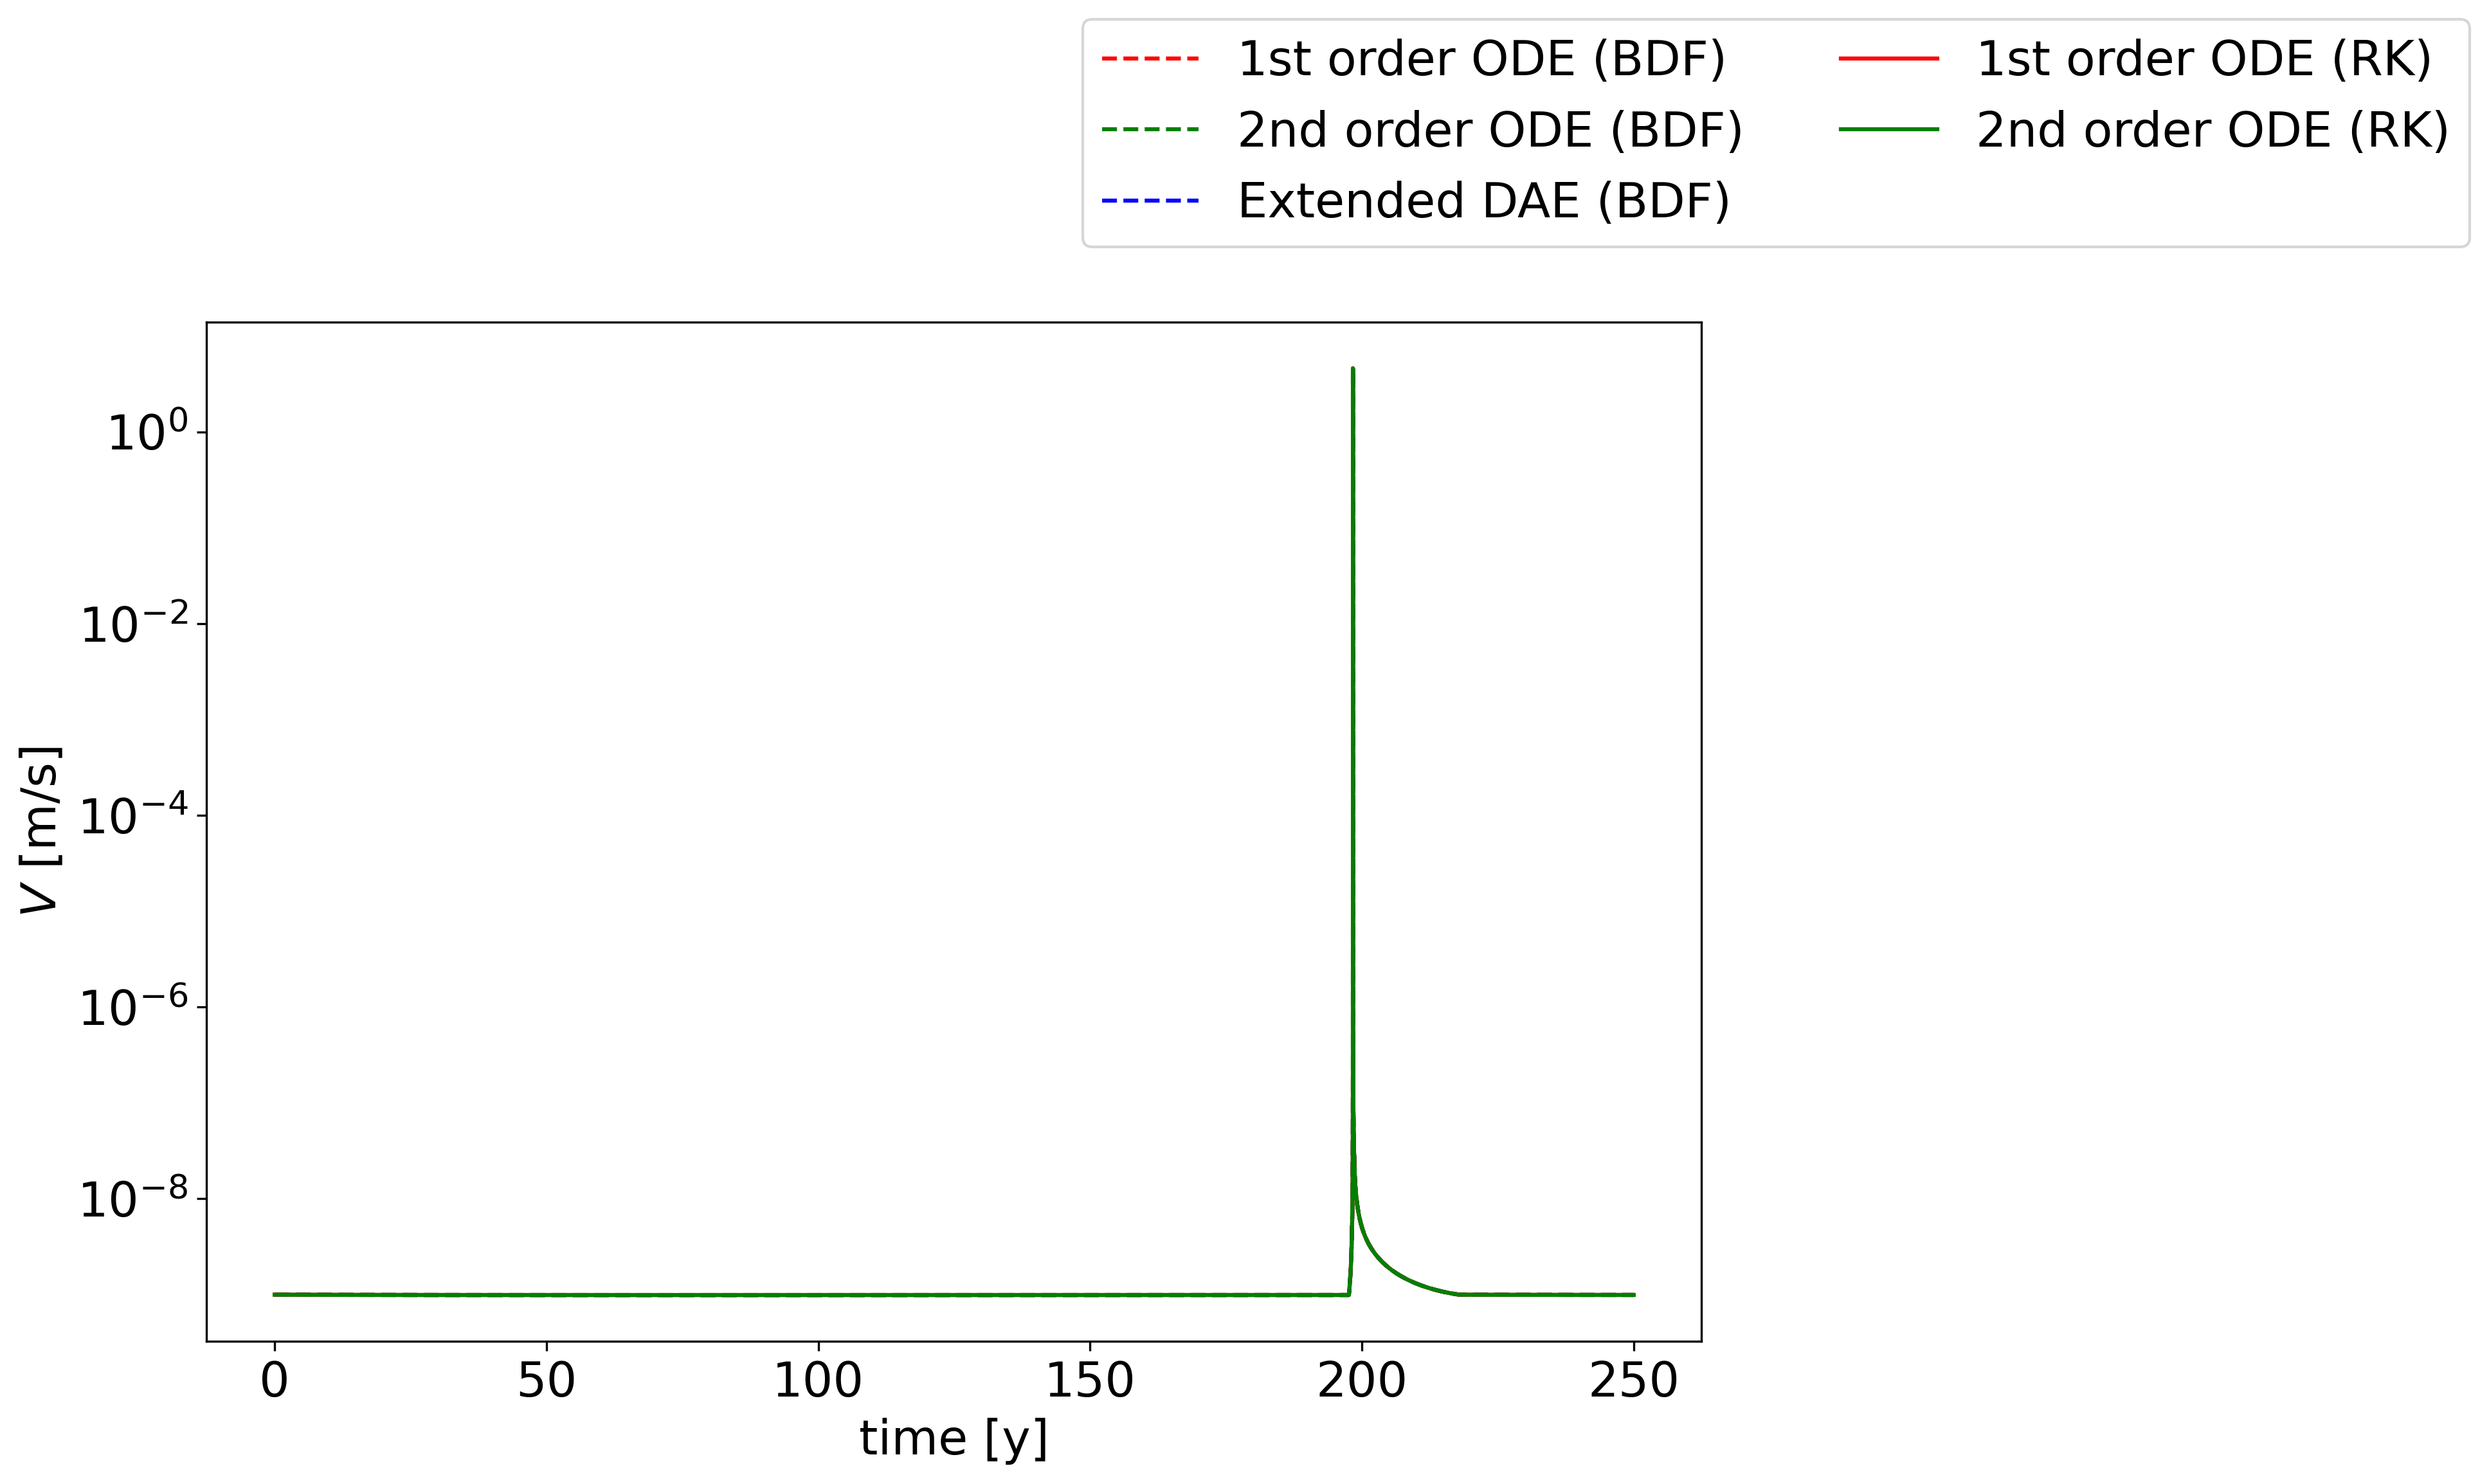
\includegraphics[width=1.45\textwidth]{images/TANDEMtimeEvolution_2D_maxSlipRate_allFormulations.png}
       	\subcaption{Full simulation time} 
    \end{subfigure} 
    \begin{subfigure}[b]{0.45\textwidth}
    	\centering
    	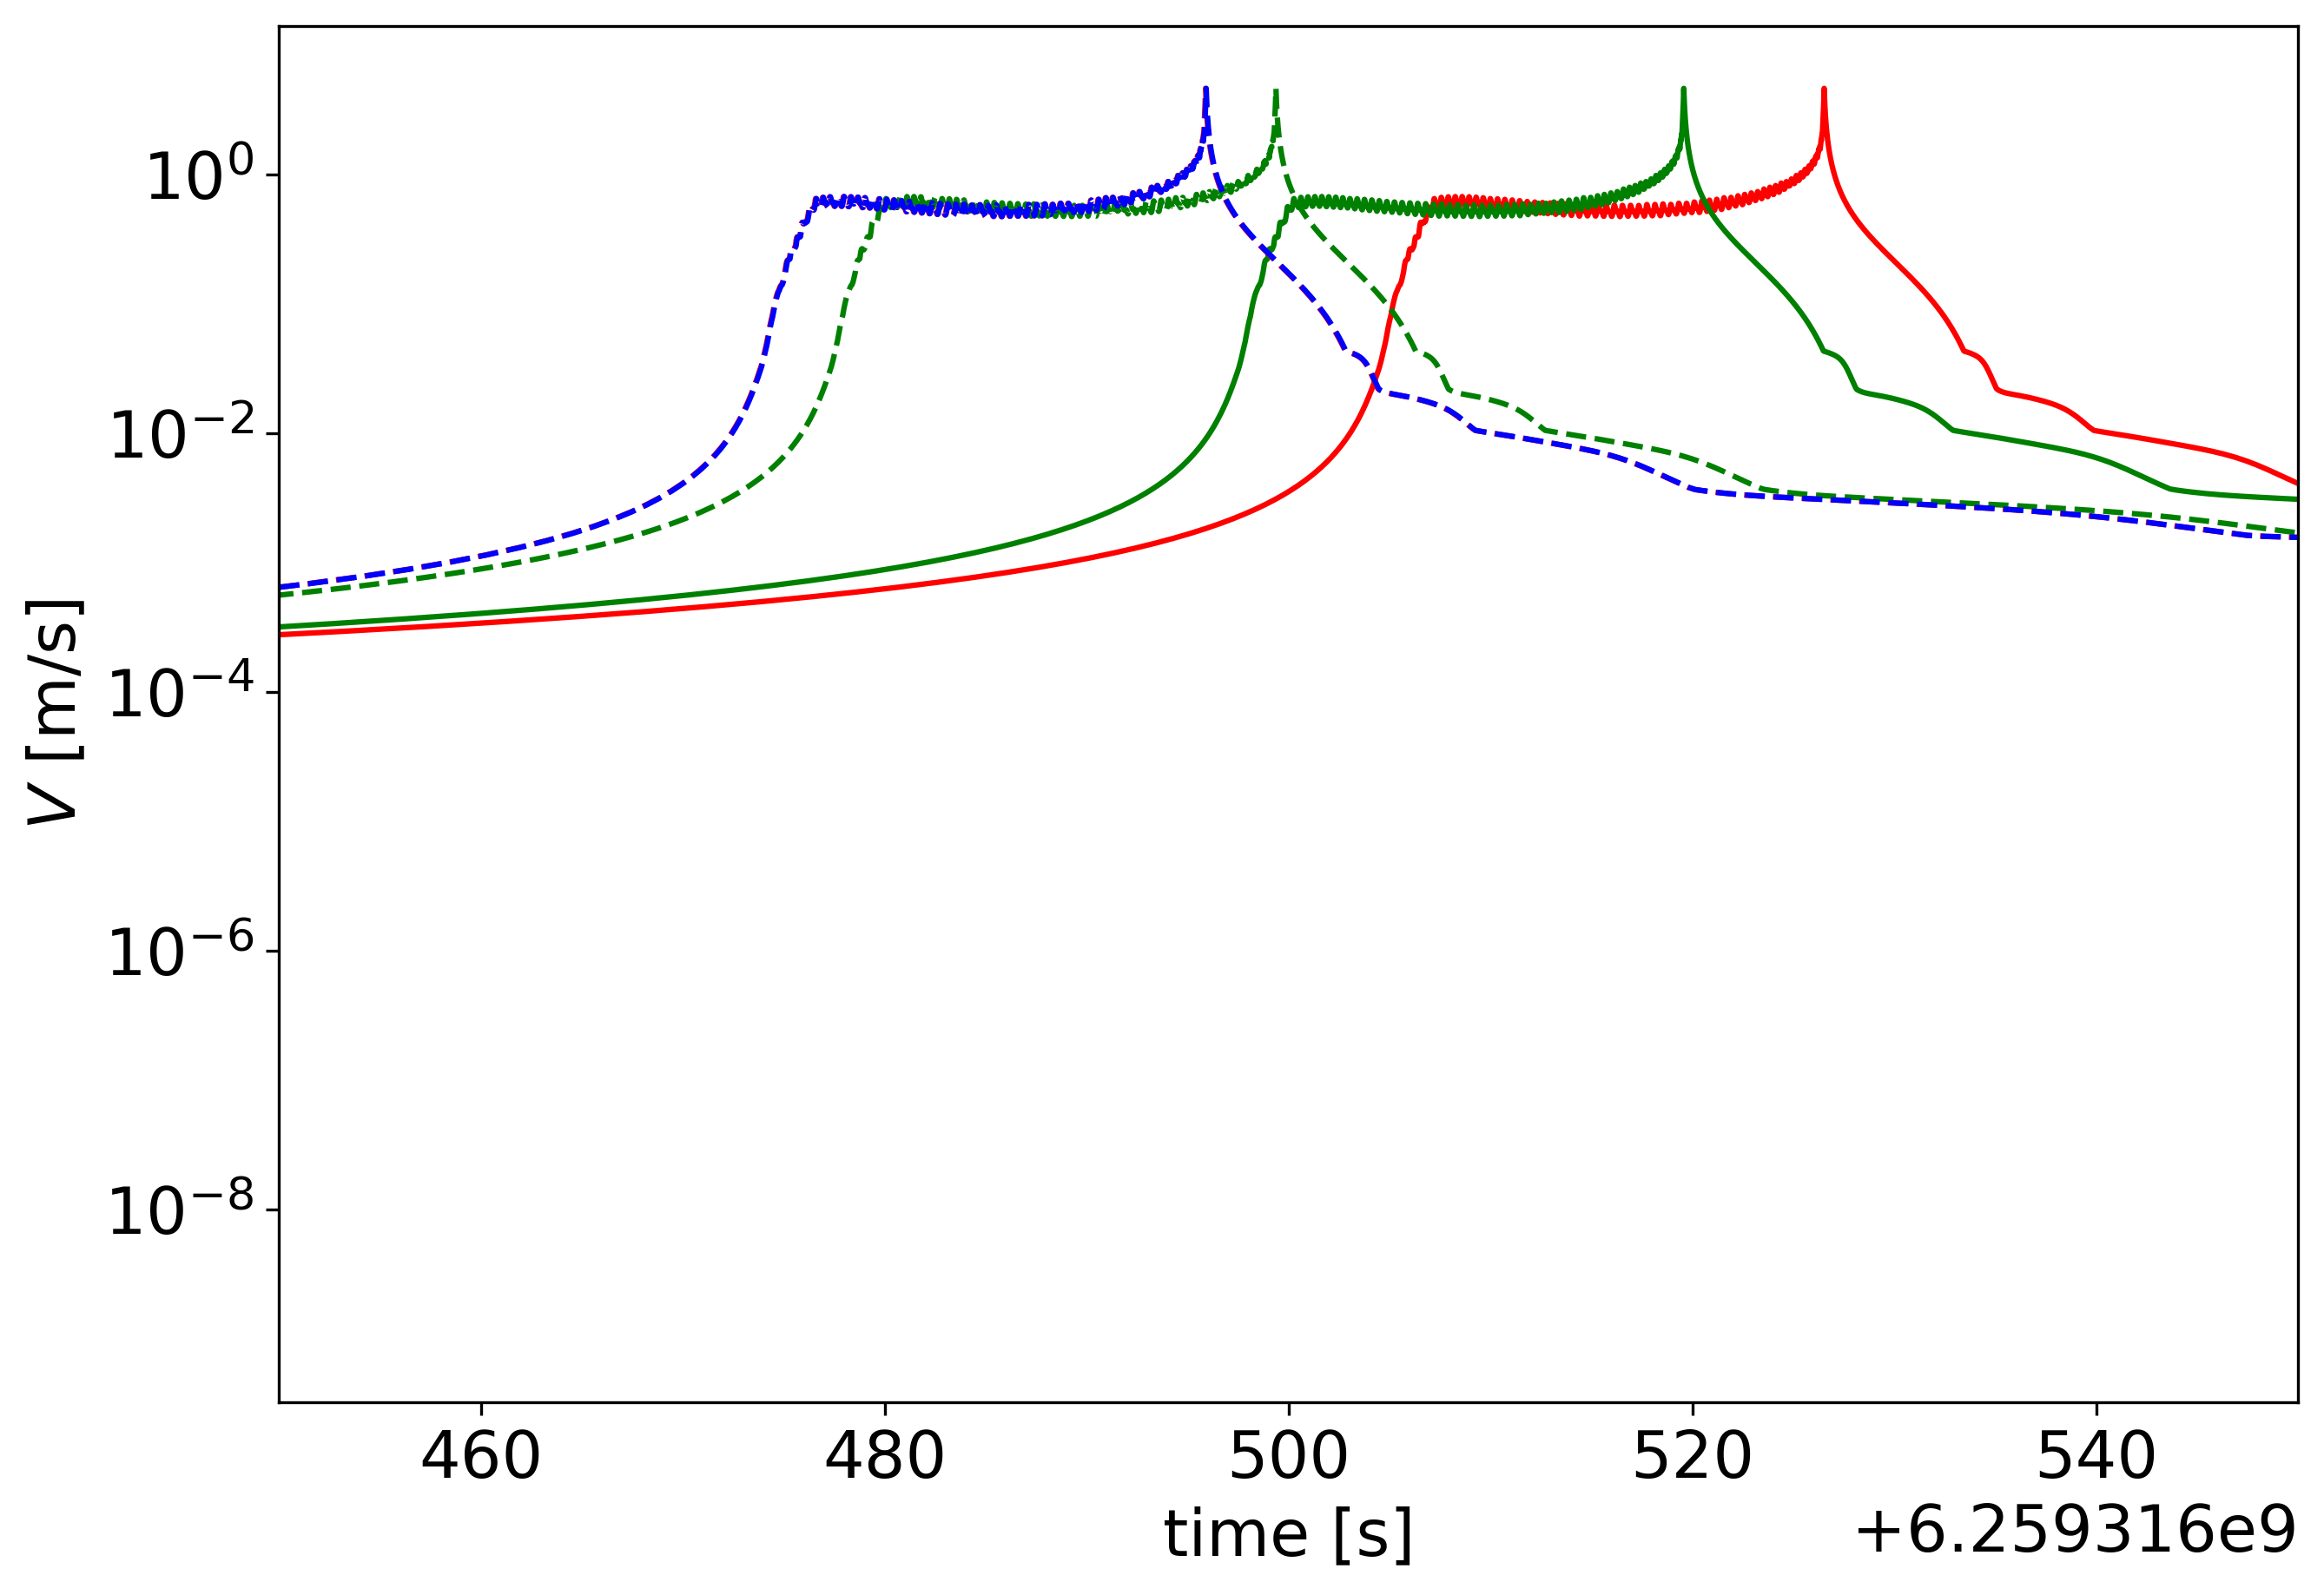
\includegraphics[width=1\textwidth]{images/TANDEMtimeEvolution_2D_maxSlipRate_allFormulations_Earthquake.png}
       	\subcaption{Close-up onto the earthquake event} 
    \end{subfigure}
    \caption{Evolution of the maximal slip rate $V$ on the fault for different solvers on the symmetric two-dimensional BP1 problem with 200 fault elements}
    \label{fig:timeEvolutionTANDEM_V}
\end{figure}


\section{Accuracy of the time integration}
\label{sec:Results_AccuracyTimeIntegration}
The discussion in \autoref{ssec:LowerBoundTimeTolerance} tackled the question of the smallest possible tolerances to reach as accurate results as possible. However, such strict tolerances may severely reduce the timestep size and by consequence the duration of the simulation. For many applications, satisfactory results are already obtained for larger tolerances, and this section aims to investigate it for SEAS. As there is no mathematical definition for \textit{satisfactory results} (unless convergence is the only requirement), the simulations are run with the strictest possible tolerance described in the previous section and assess how the results deteriorate as the tolerances increase.

\subsection{First order formulations}
First, the impact of the tolerance value is investigated on a domain with 101 fault elements using the 1st order ODE formulation. The analysis considers the aseismic and the earthquake phases separately, since they have different requirements. The former is accurate if earthquakes are predicted at the correct time, whereas the latter is accurate if the earthquake is correctly simulated in terms of slip rate and total increase of the slip. We use here the flexibility of the implementation of defining different tolerances for the aseismic and earthquake phases.

\subsubsection{Aseismic slip}
In the first set of experiments, the reference solution corresponds to the absolute tolerances $t_a^S =10^{-11}$ and $t_a^\psi =10^{-13}$, and this tolerance is kept in the earthquake phase for all simulation runs. The simulated time is increased to 300 years such that two earthquake events can be observed after 204 and 270 years. As metrics for the accuracy, we take the time of the first earthquake, to investigate the initial slip, then we take the period between the two earthquakes. These metrics are appropriate, because the focus now is on the aseismic slip, in which stress builds up until an earthquake is triggered, and an accurate simulation environment should detect the same earthquakes at the same simulated times. The results are collected in \autoref{fig:tolerancesAseismicSlip_compactODE} for both the explicit, 5th order, Dormand-Prince RK method and the implicit, adaptive-order, BDF scheme. 
\begin{figure}[H]
	\centering
	\begin{subfigure}[t]{0.32\textwidth}
		\centering
		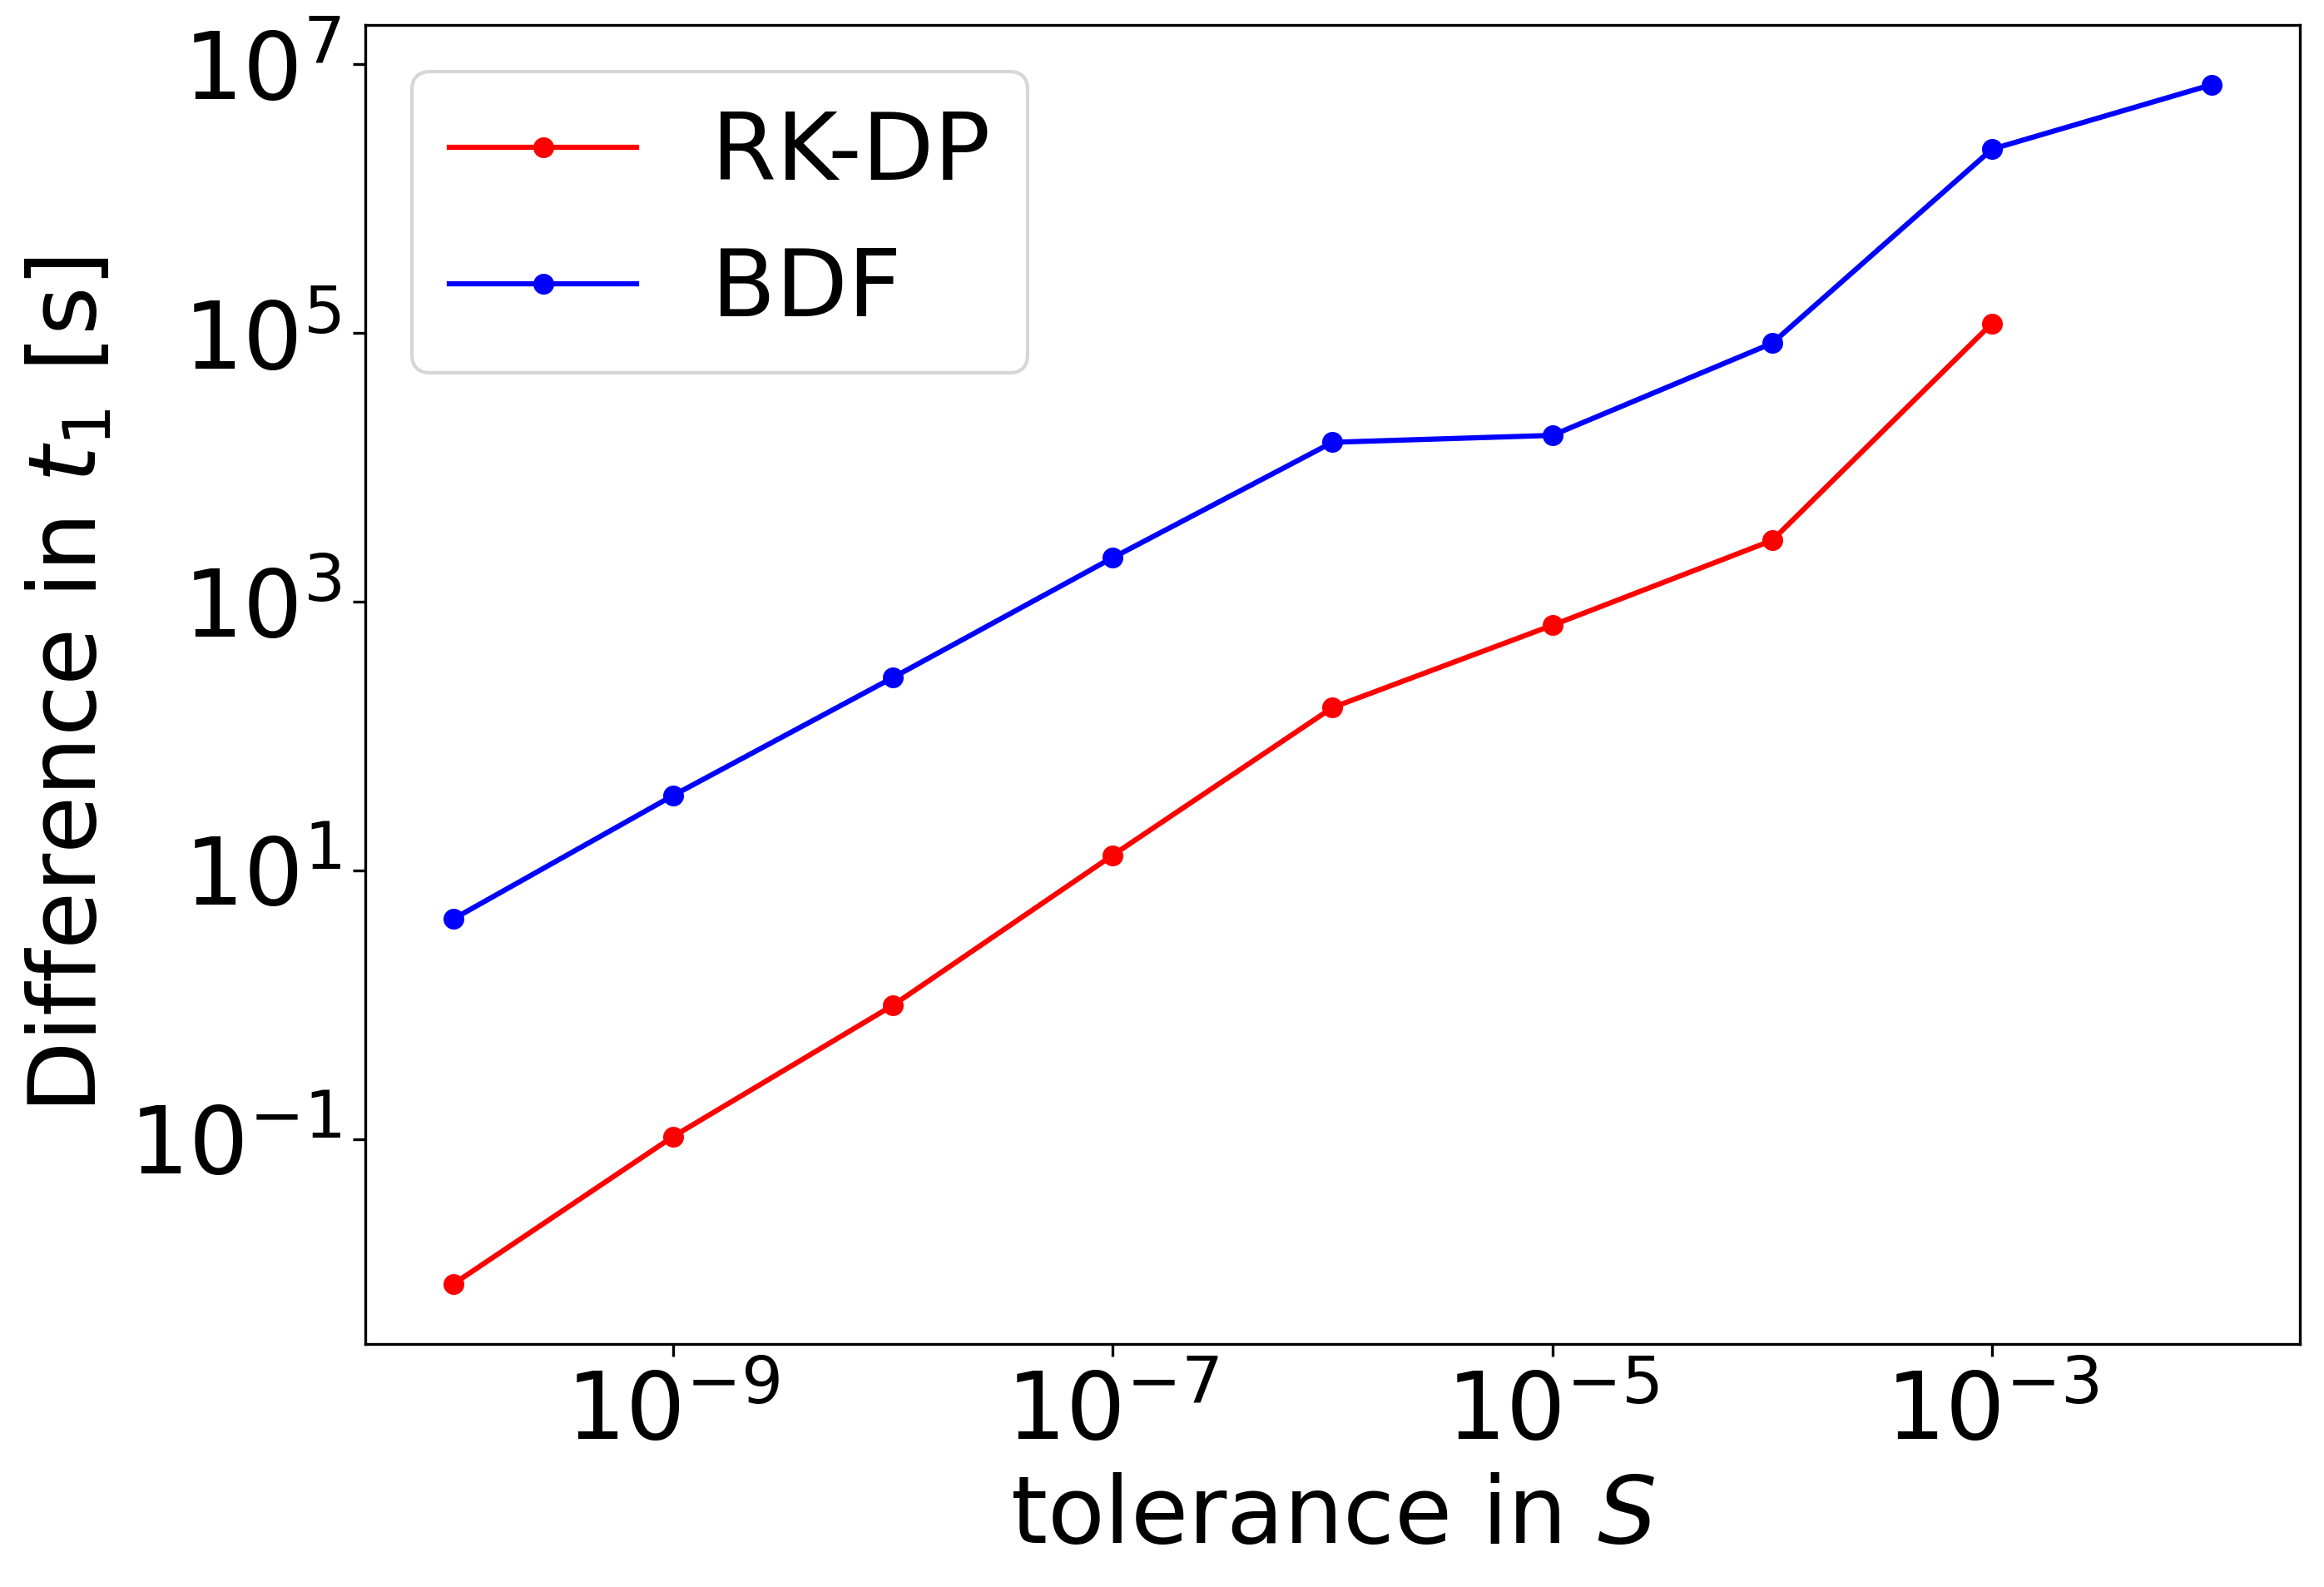
\includegraphics[width=1\textwidth]{images/TANDEMcompactODEDifferentTolerancesSize101_AS_FirstEarthquakeTimeDiff.png}
		\subcaption{Time difference of the \\ first earthquake} 
	\end{subfigure} 
	\begin{subfigure}[t]{0.32\textwidth}
		\centering
		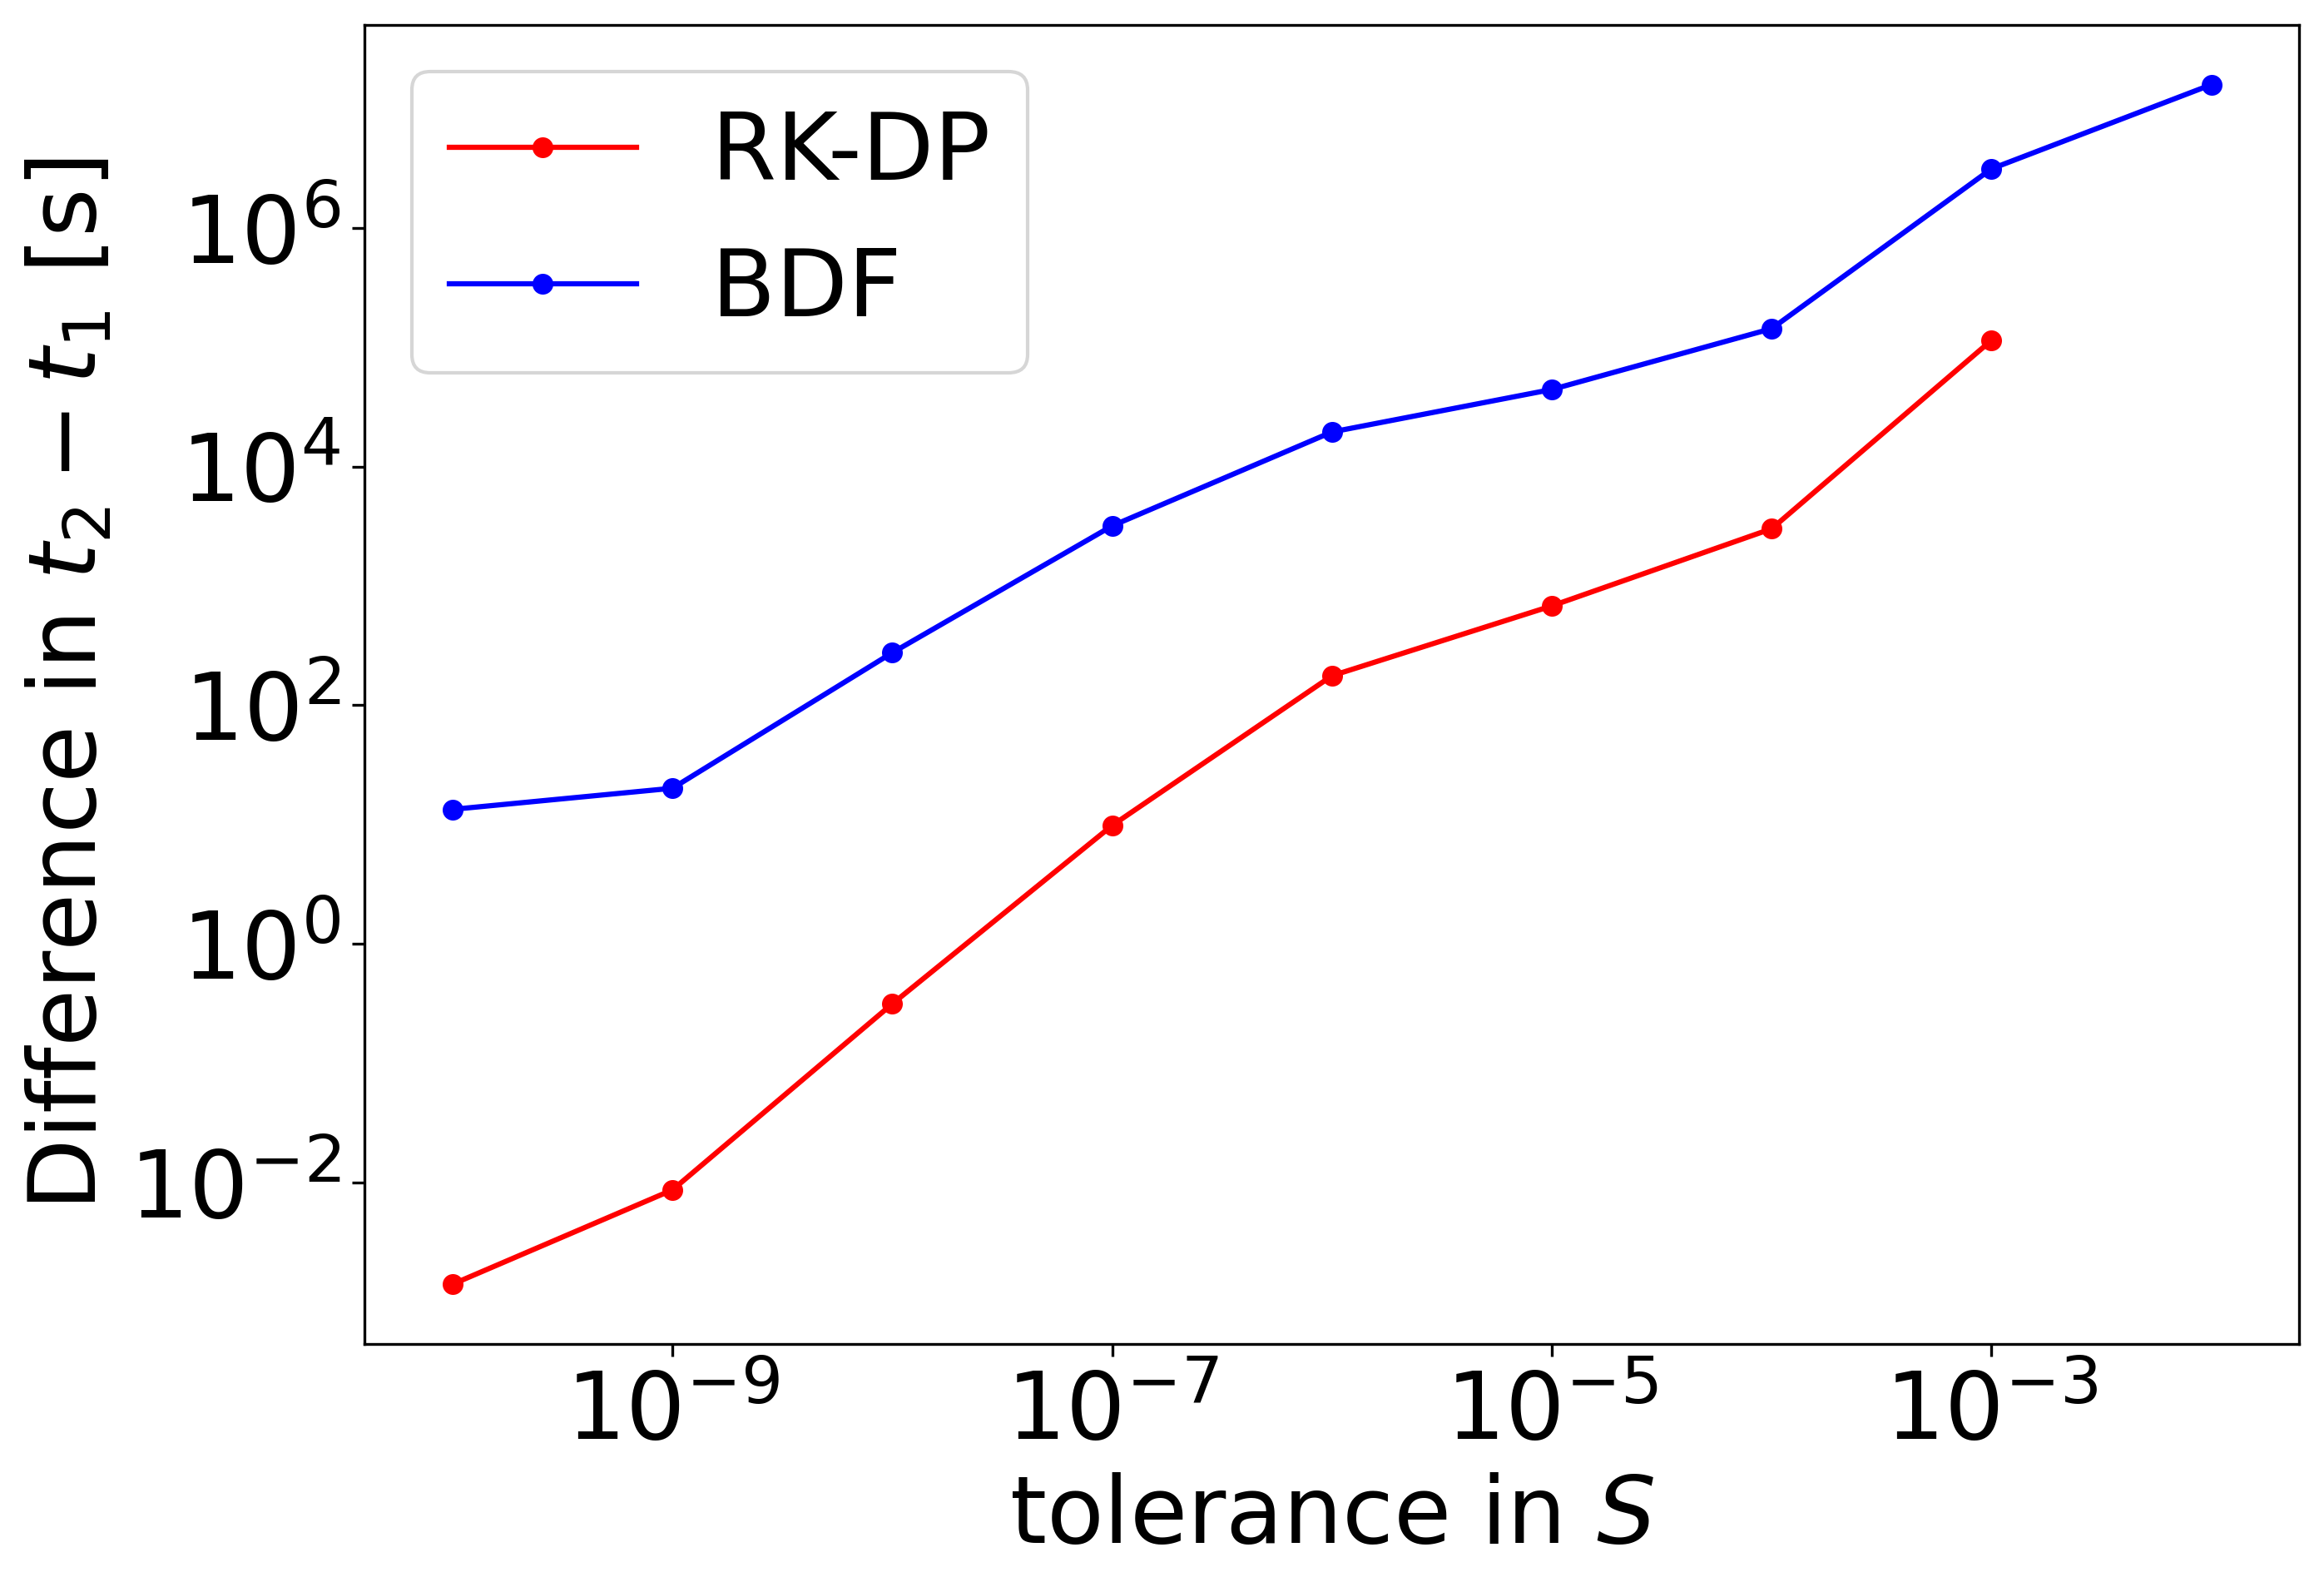
\includegraphics[width=1\textwidth]{images/TANDEMcompactODEDifferentTolerancesSize101_AS_PeriodDiff.png}
		\subcaption{Difference of the period \\ between two earthquakes} 
	\end{subfigure}
	\begin{subfigure}[t]{0.32\textwidth}
		\centering
		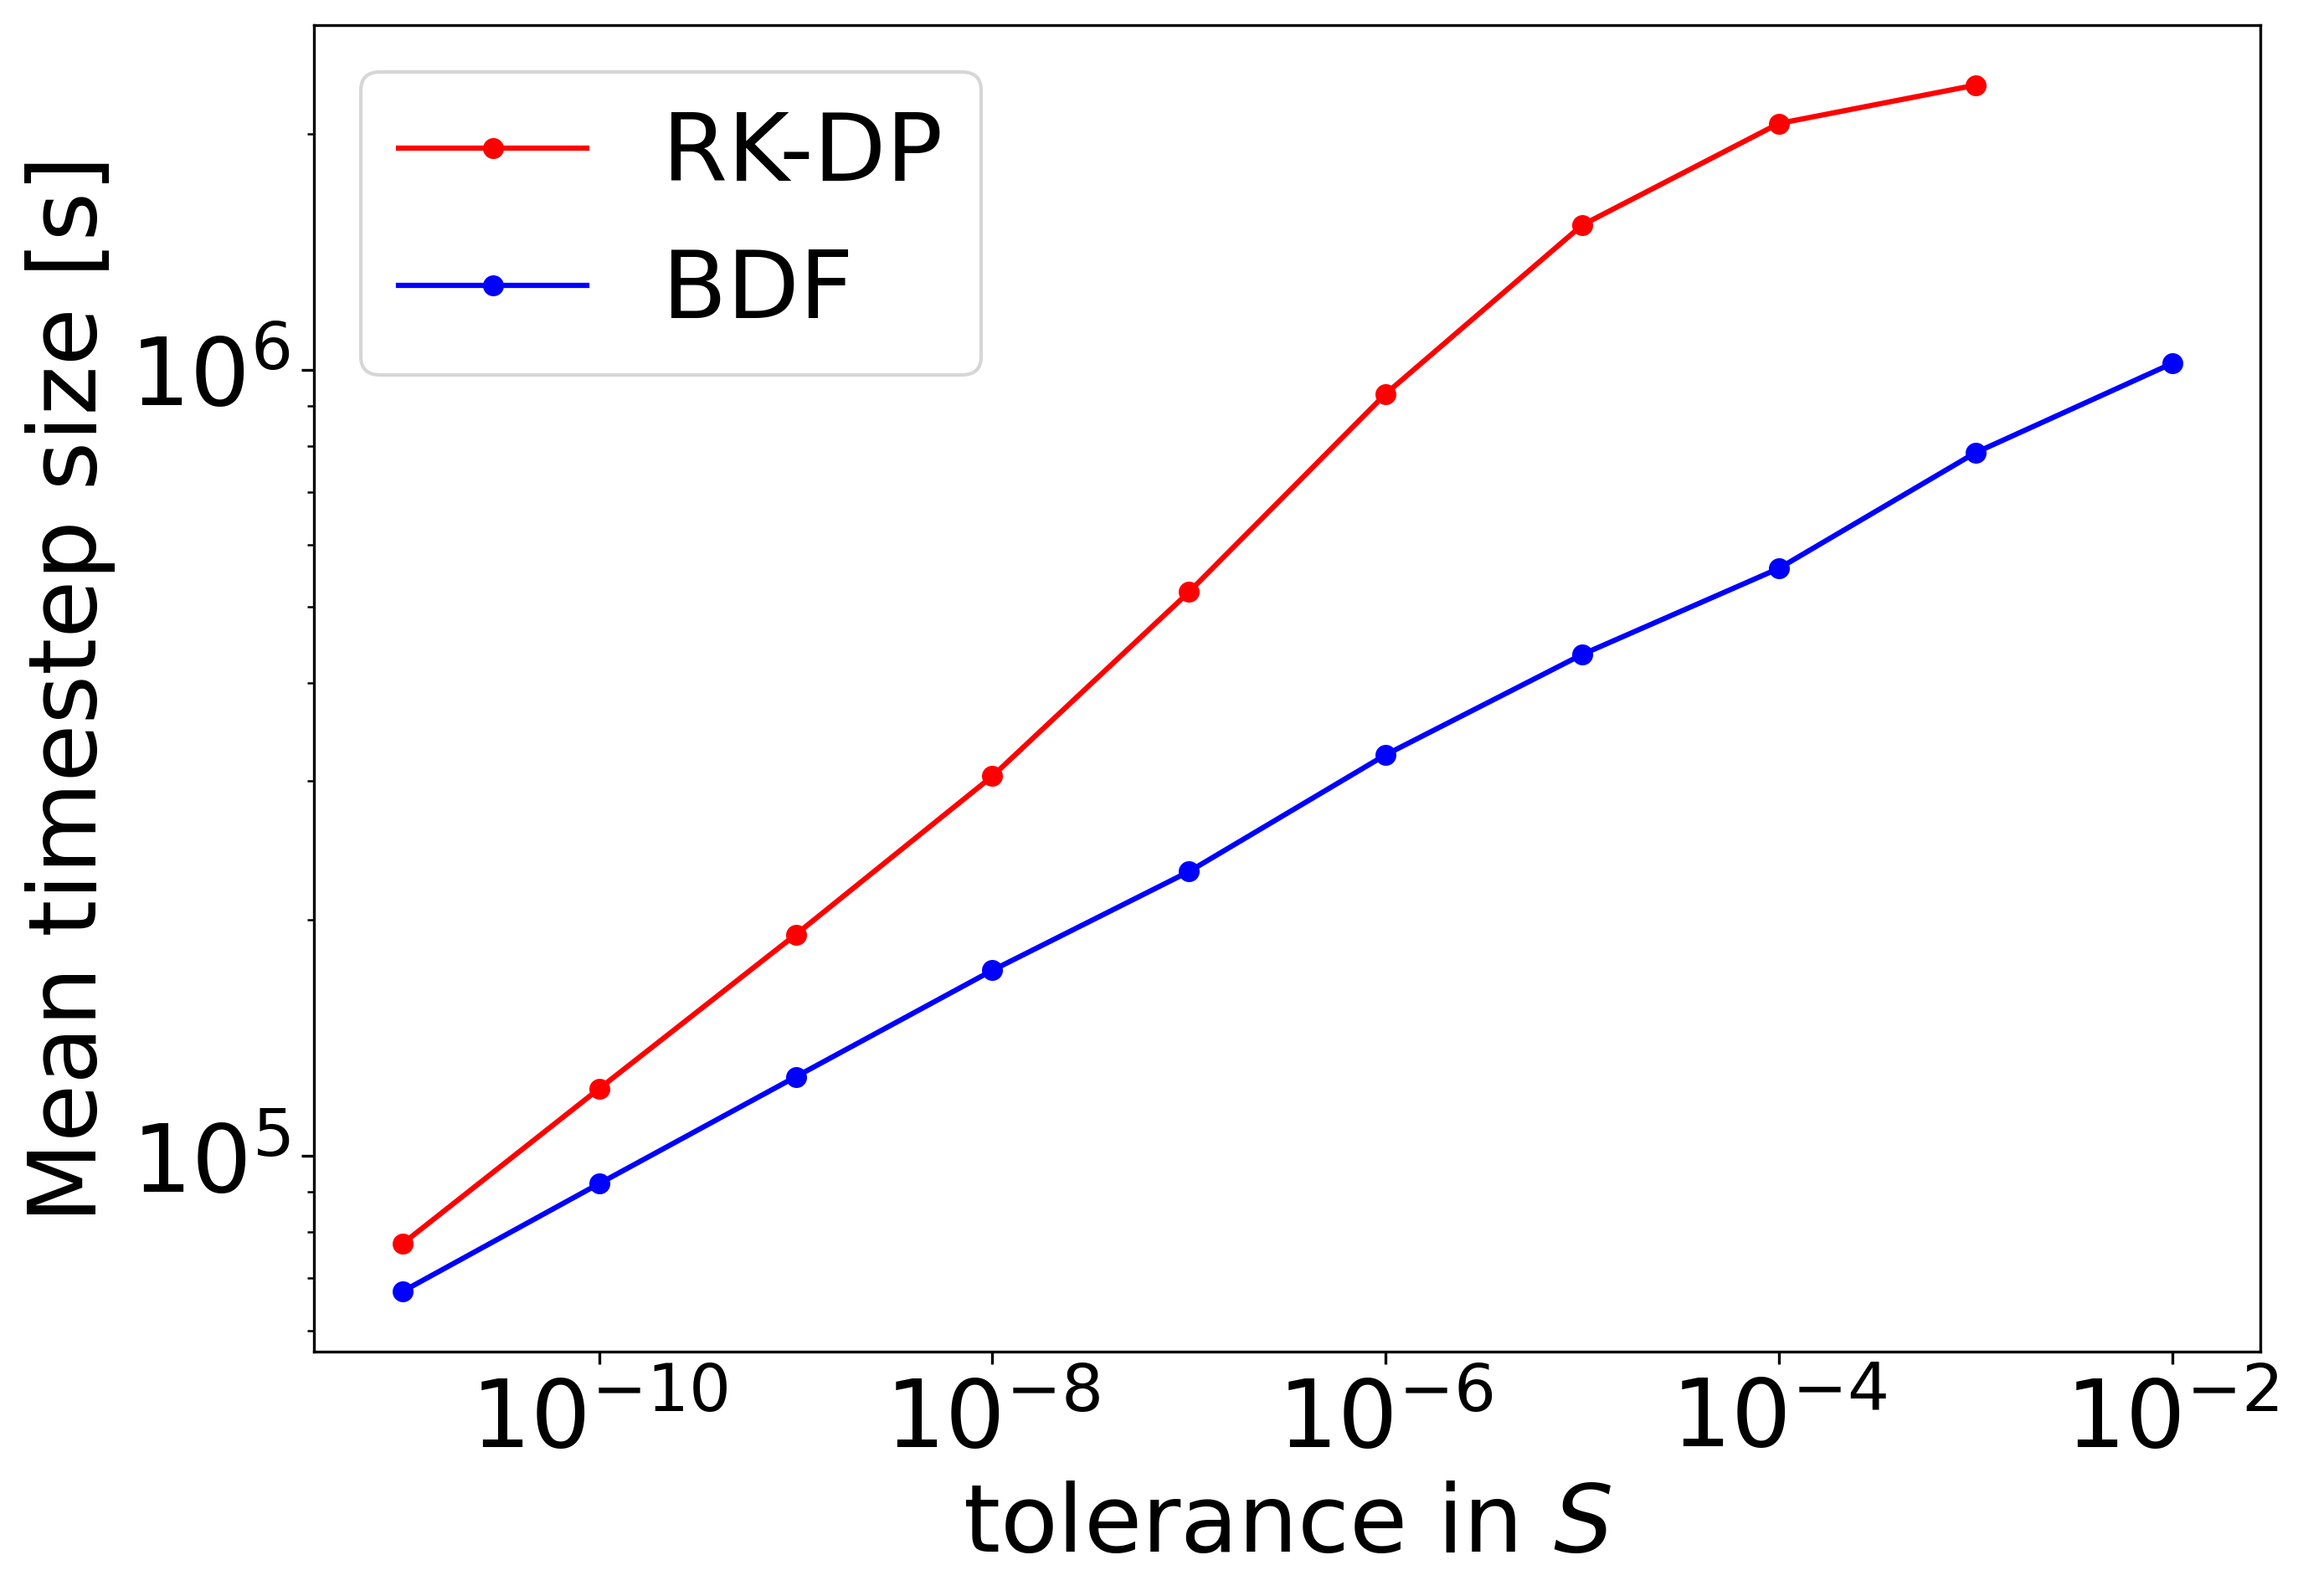
\includegraphics[width=1\textwidth]{images/TANDEMcompactODEDifferentTolerancesSize101_AS_DT.png}
		\subcaption{Geometric mean of \\ the timestep size in the \\ aseismic slip} 
	\end{subfigure}
	\caption{Difference of characteristic times for simulations with different tolerances in the aseismic slip phase to the simulation with strictest tolerance on a domain with 101 fault elements with the 1st order ODE formulation using implicit and explicit time integration schemes.}
	\label{fig:tolerancesAseismicSlip_compactODE}
\end{figure}
As expected, the accuracy of the predicted times worsens exponentially if the tolerance increases and the relationship. However, it appears that the implicit method deteriorates faster than the explicit. To achieve the earthquake within one hour (=3600s) of its actual occurrence, the necessary tolerances are:  
\begin{itemize}
	\item RK method: $t_a^S<10^{-5}$m
	\item BDF method: $t_a^S<10^{-7}$m
\end{itemize}
Considering the 200 years of simulated time, this is a very small error and an even larger tolerance may be acceptable for some simulations. Remember that in \autoref{sec:2DSEAS__EvolutionOfQuantities} the earthquake got shifted by two and a half years if the number of fault elements is doubled, thus the error induced by the DG scheme is larger by magnitudes.  \\
It appears that the RK method fails if the tolerance exceeds $10^{-3}$m, which is not the case for the BDF method. Indeed, in the last few timesteps, before the earthquake is triggered, the built-in iterative solver for the friction returns wrong values for $V$ until NaNs are encountered. In BDF, the residual of the Newton iteration diverges right away with wrong slip rates, and the timestep size is scaled down in time. However, at $t_a^S = 10^{-2}$m, which can only be reached with implicit methods, the times are already off by $10^7$s $\approx 116$days and thus of the same order of magnitude as the error observed with a coarser mesh resolution. \\

\subsection{Earthquake phase}
In the second set experiments, the tolerances for the aseismic phase are kept constant and tolerances in the earthquake phase are progressively decreased. The simulation time is put back to 250 years, such that only one earthquake occurs. There are two quantities of interest: the overall maximum sliprate, which represents the intensity of the earthquake, and the increase of the slip rate at open surface. The latter directly impacts the prediction of subsequent earthquakes. A small increase indicates an incomplete earthquake, where the next event happens sooner. Inversely, a strong increase delays the following earthquake. It is measured as the difference between the minimum slip at the end and the beginning of the simulation, which lie both in the aseismic phase surrounding the earthquake. \\
The accuracy is thus estimated as a combination of the intensity and the geological changes in the earthquake. The results are found in \autoref{fig:tolerancesEarthquake_compactODE} for the RK-DP and BDF schemes.

\begin{figure}[H]
	\centering
	\begin{subfigure}[t]{0.32\textwidth}
		\centering
		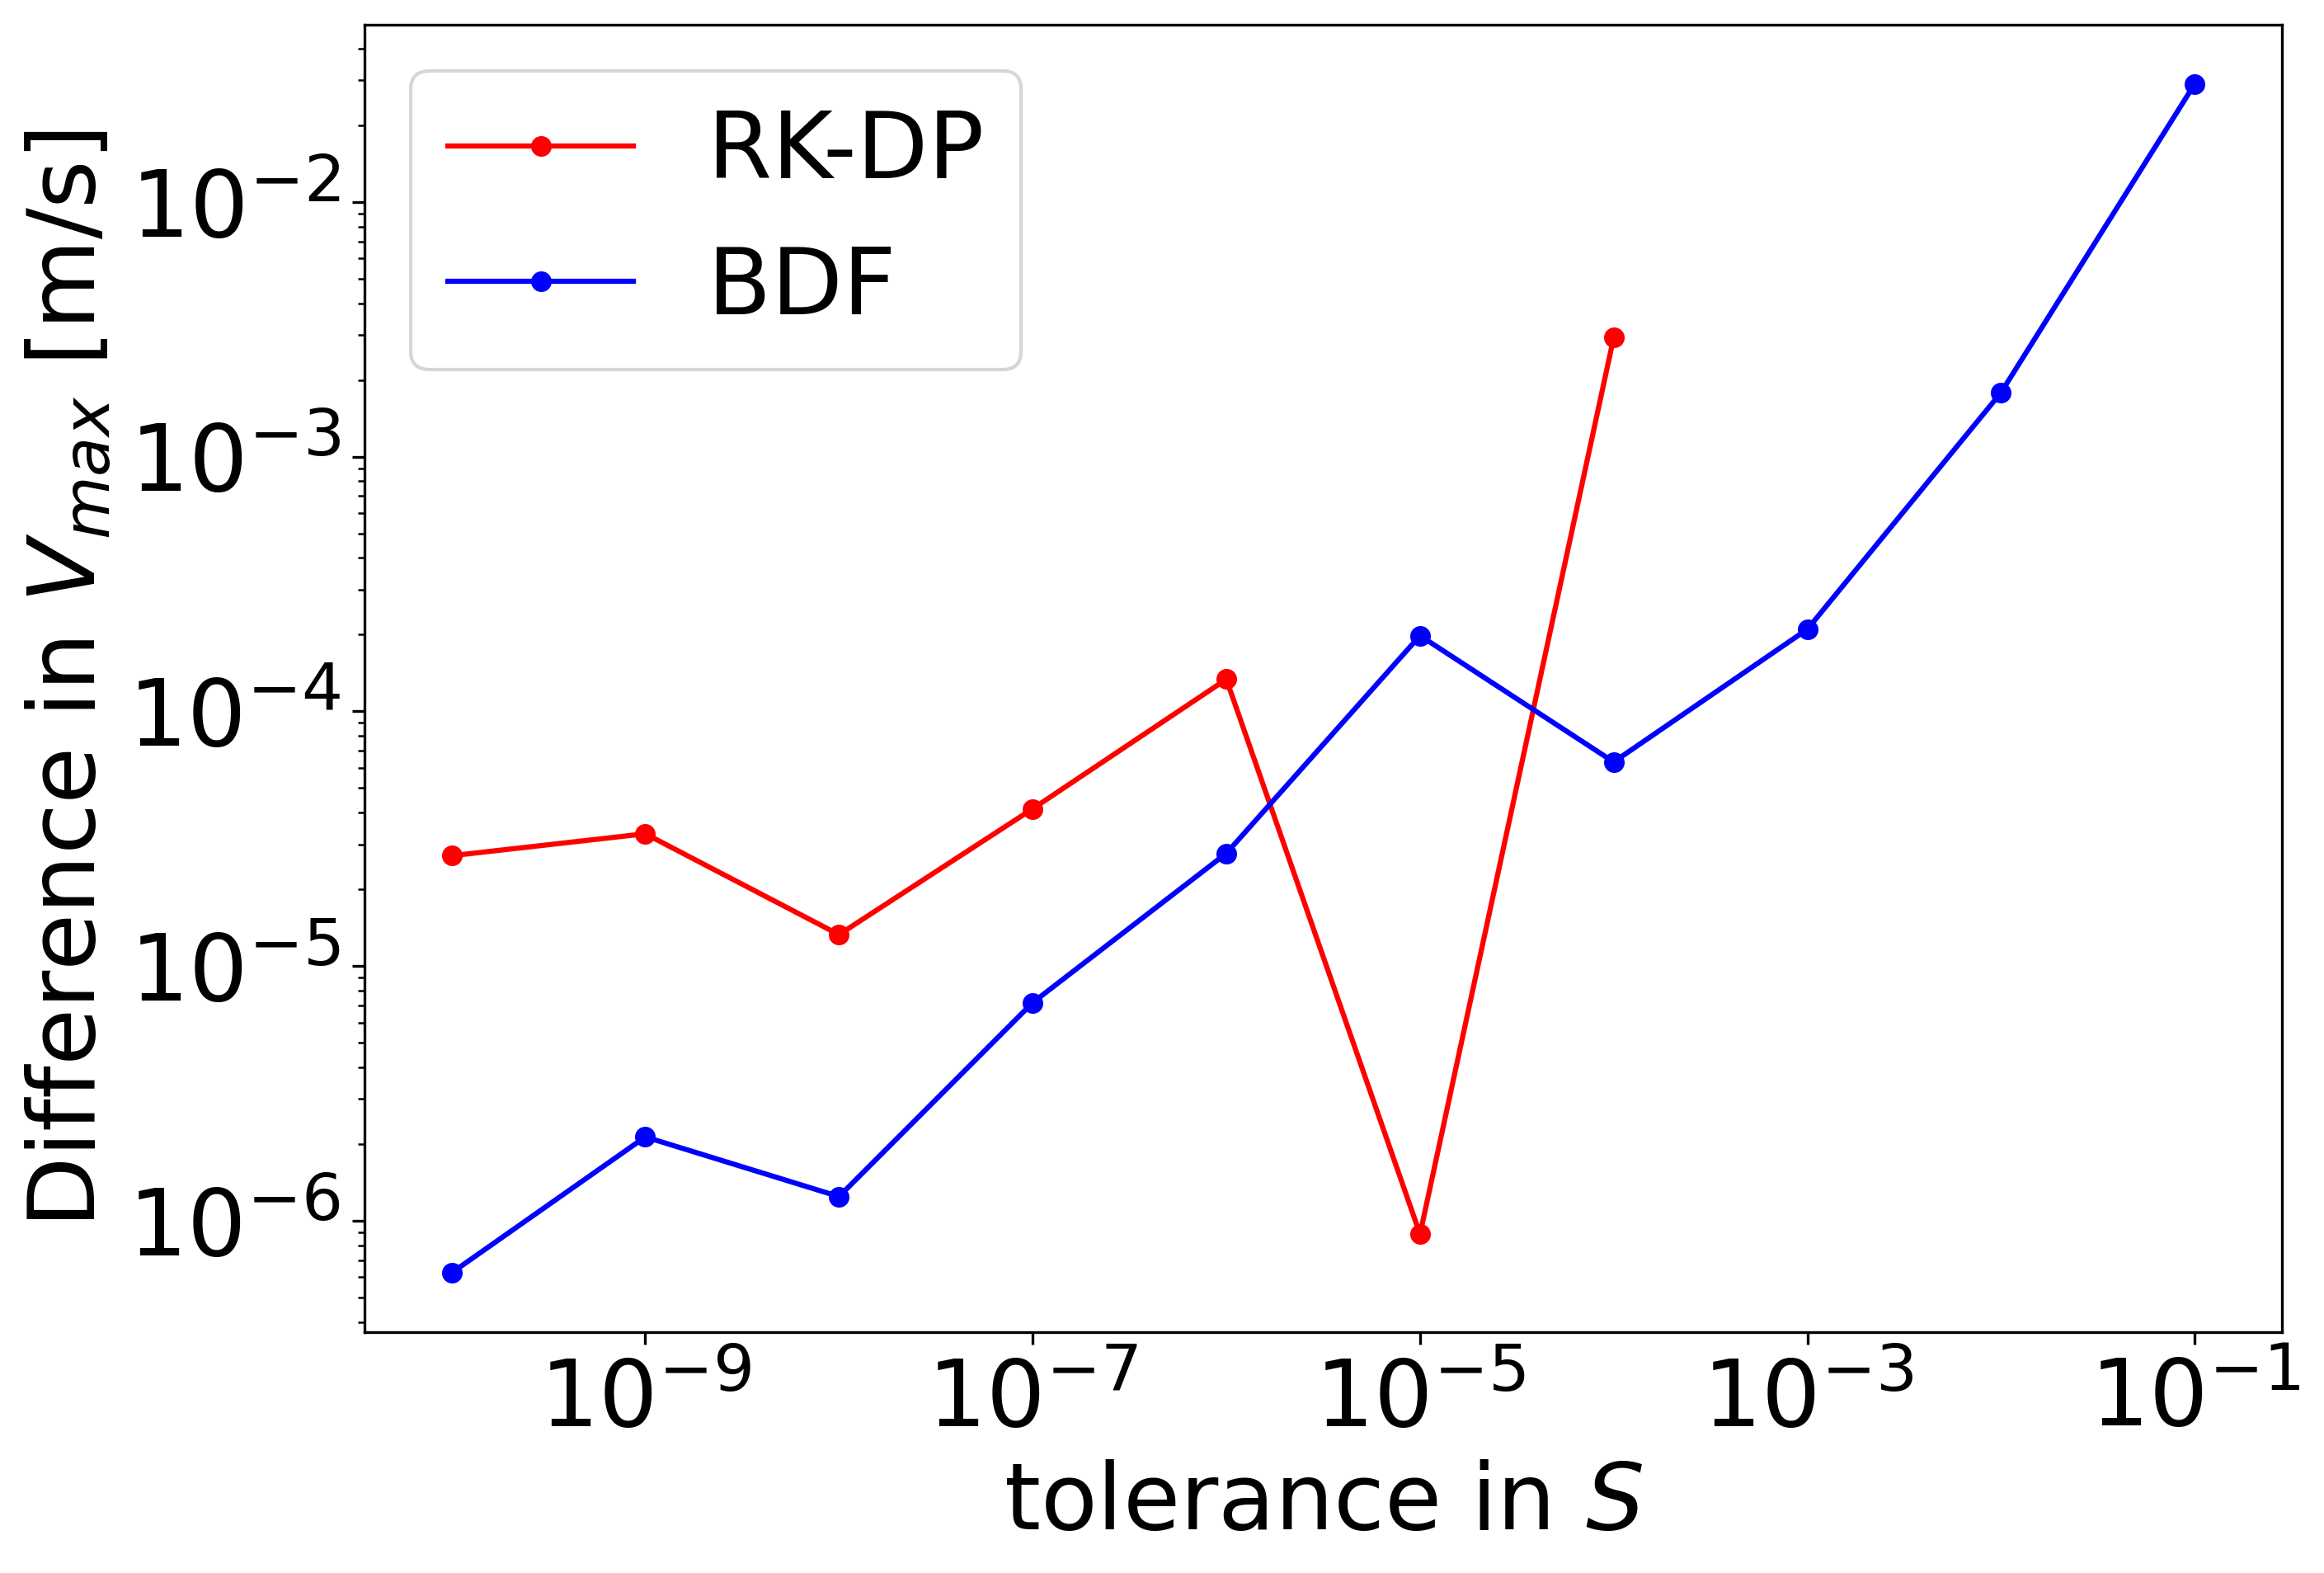
\includegraphics[width=1\textwidth]{images/TANDEMcompactODEDifferentTolerancesSize101_EQ_Vmax.png}
		\subcaption{Difference in the maximum slip rate} 
	\end{subfigure} 
	\begin{subfigure}[t]{0.32\textwidth}
		\centering
		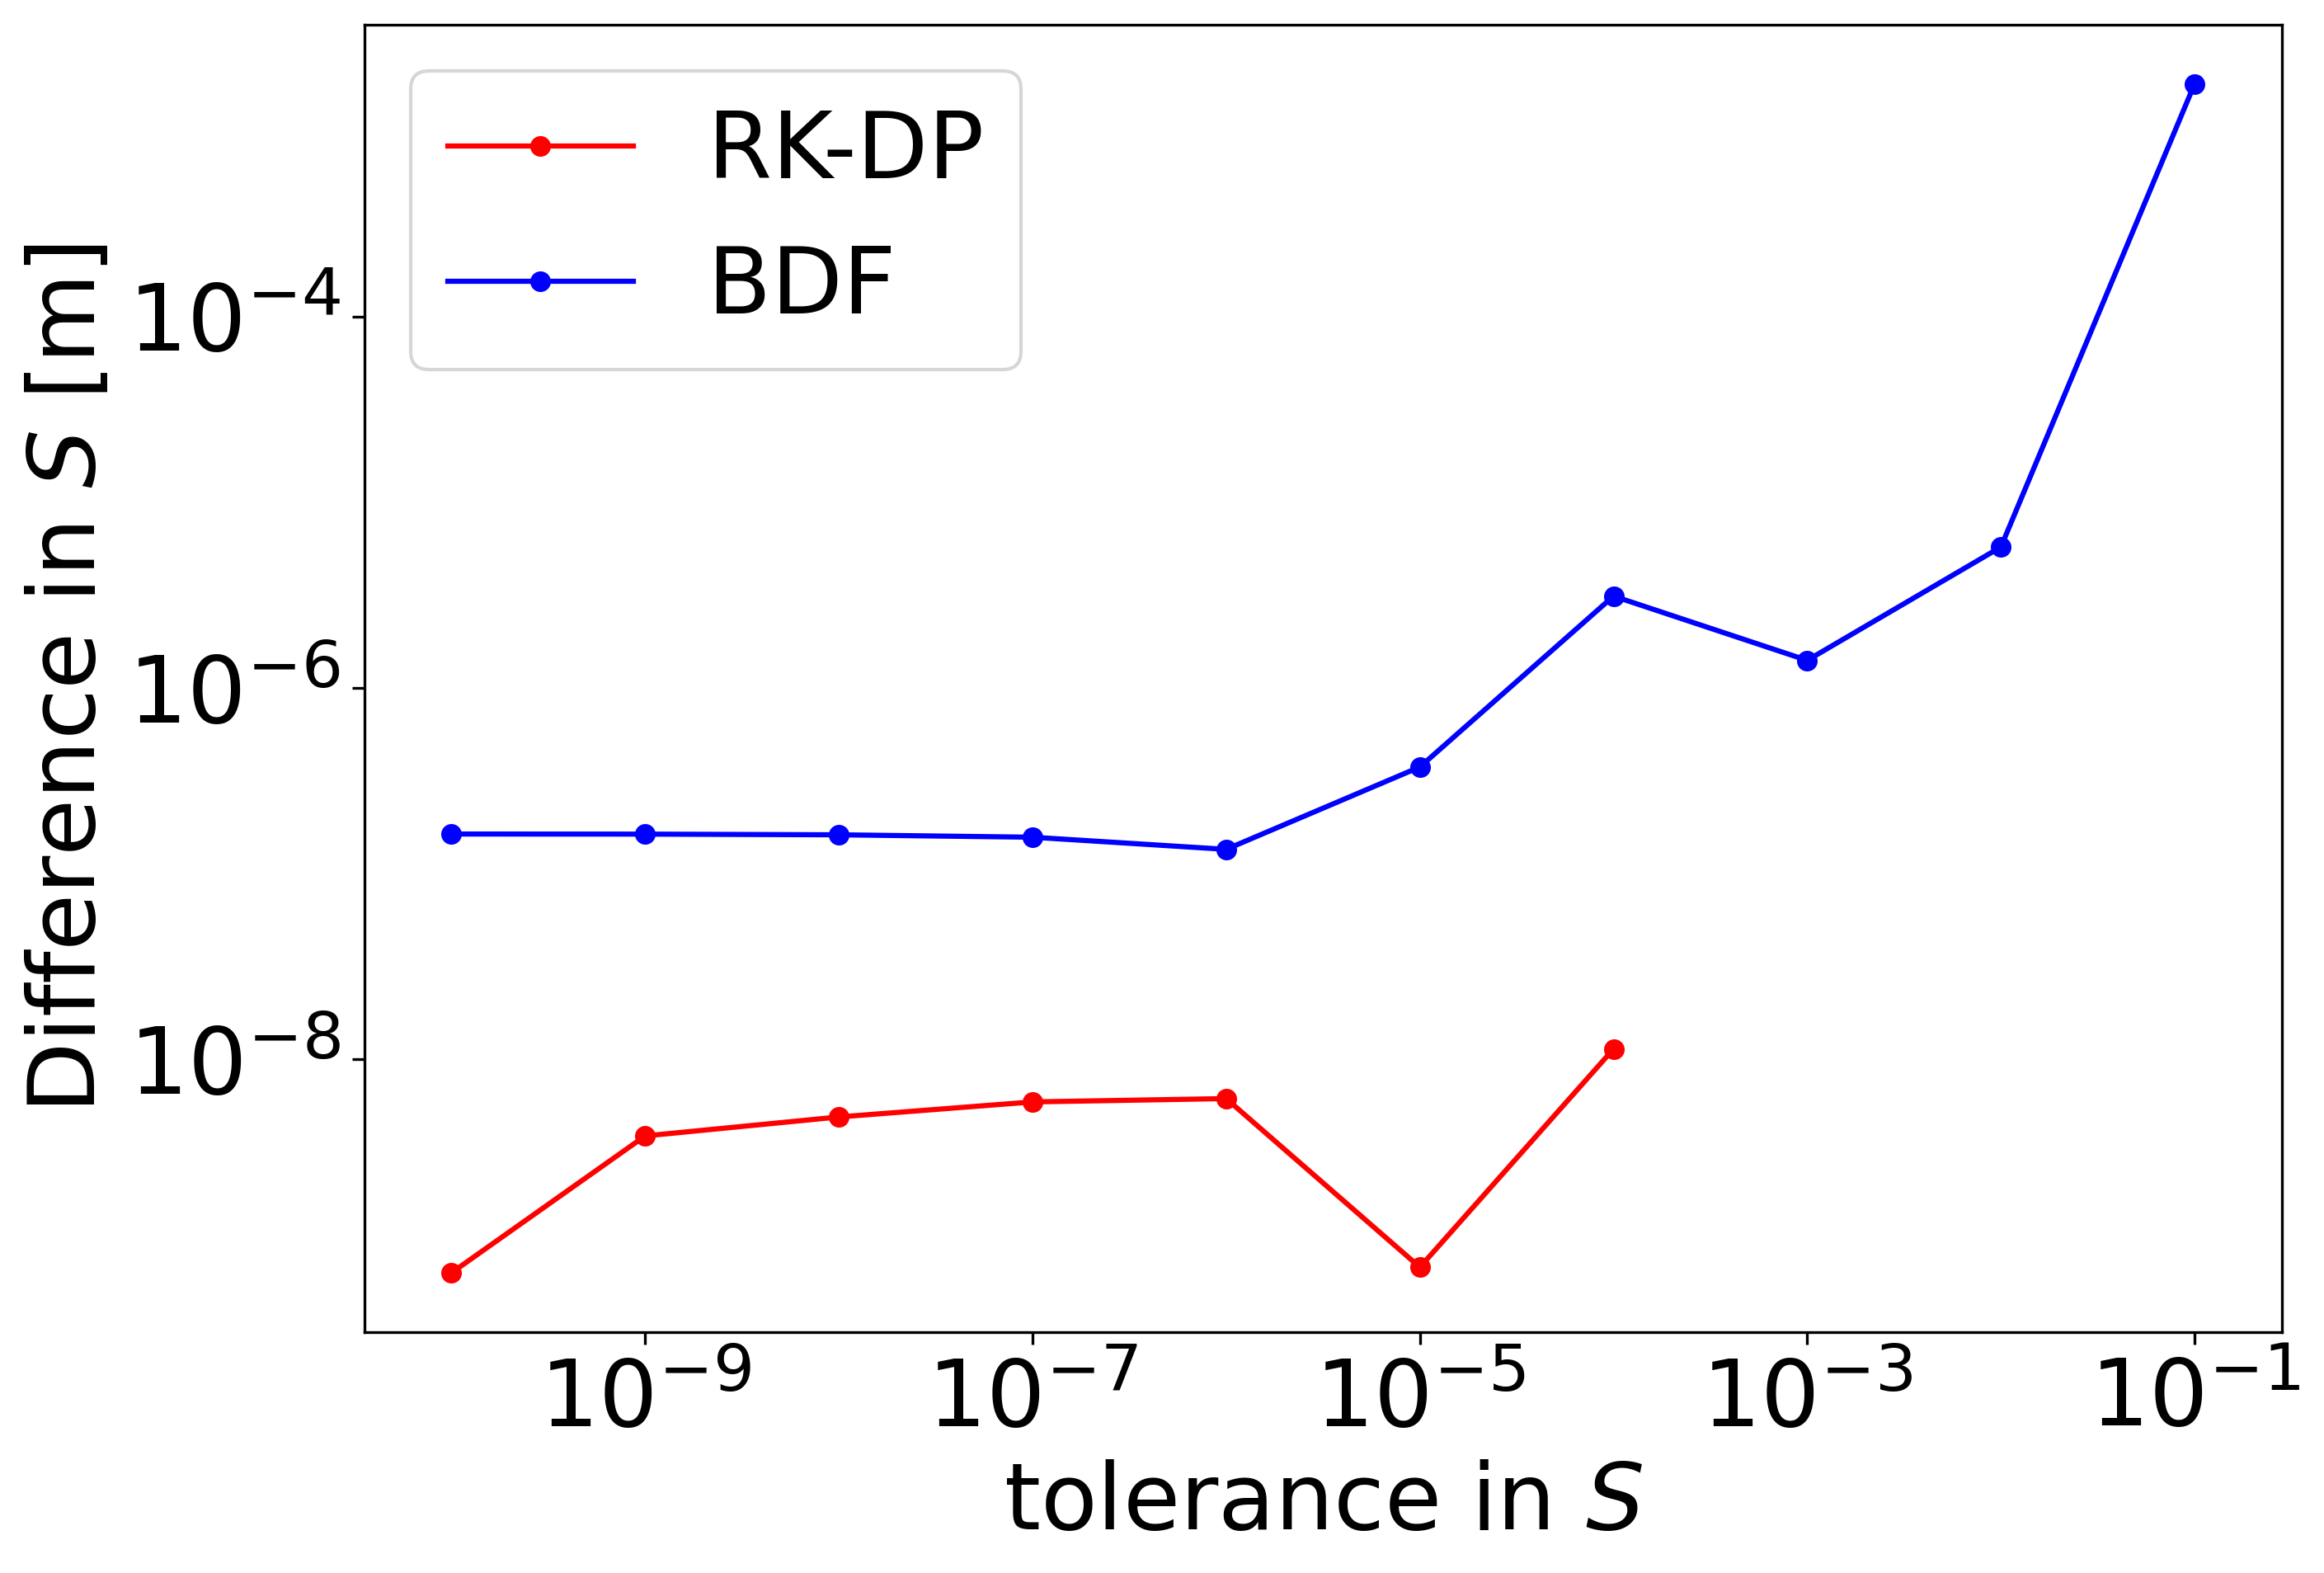
\includegraphics[width=1\textwidth]{images/TANDEMcompactODEDifferentTolerancesSize101_EQ_Smin.png}
		\subcaption{Difference in the slip increase} 
	\end{subfigure}
	\begin{subfigure}[t]{0.32\textwidth}
		\centering
		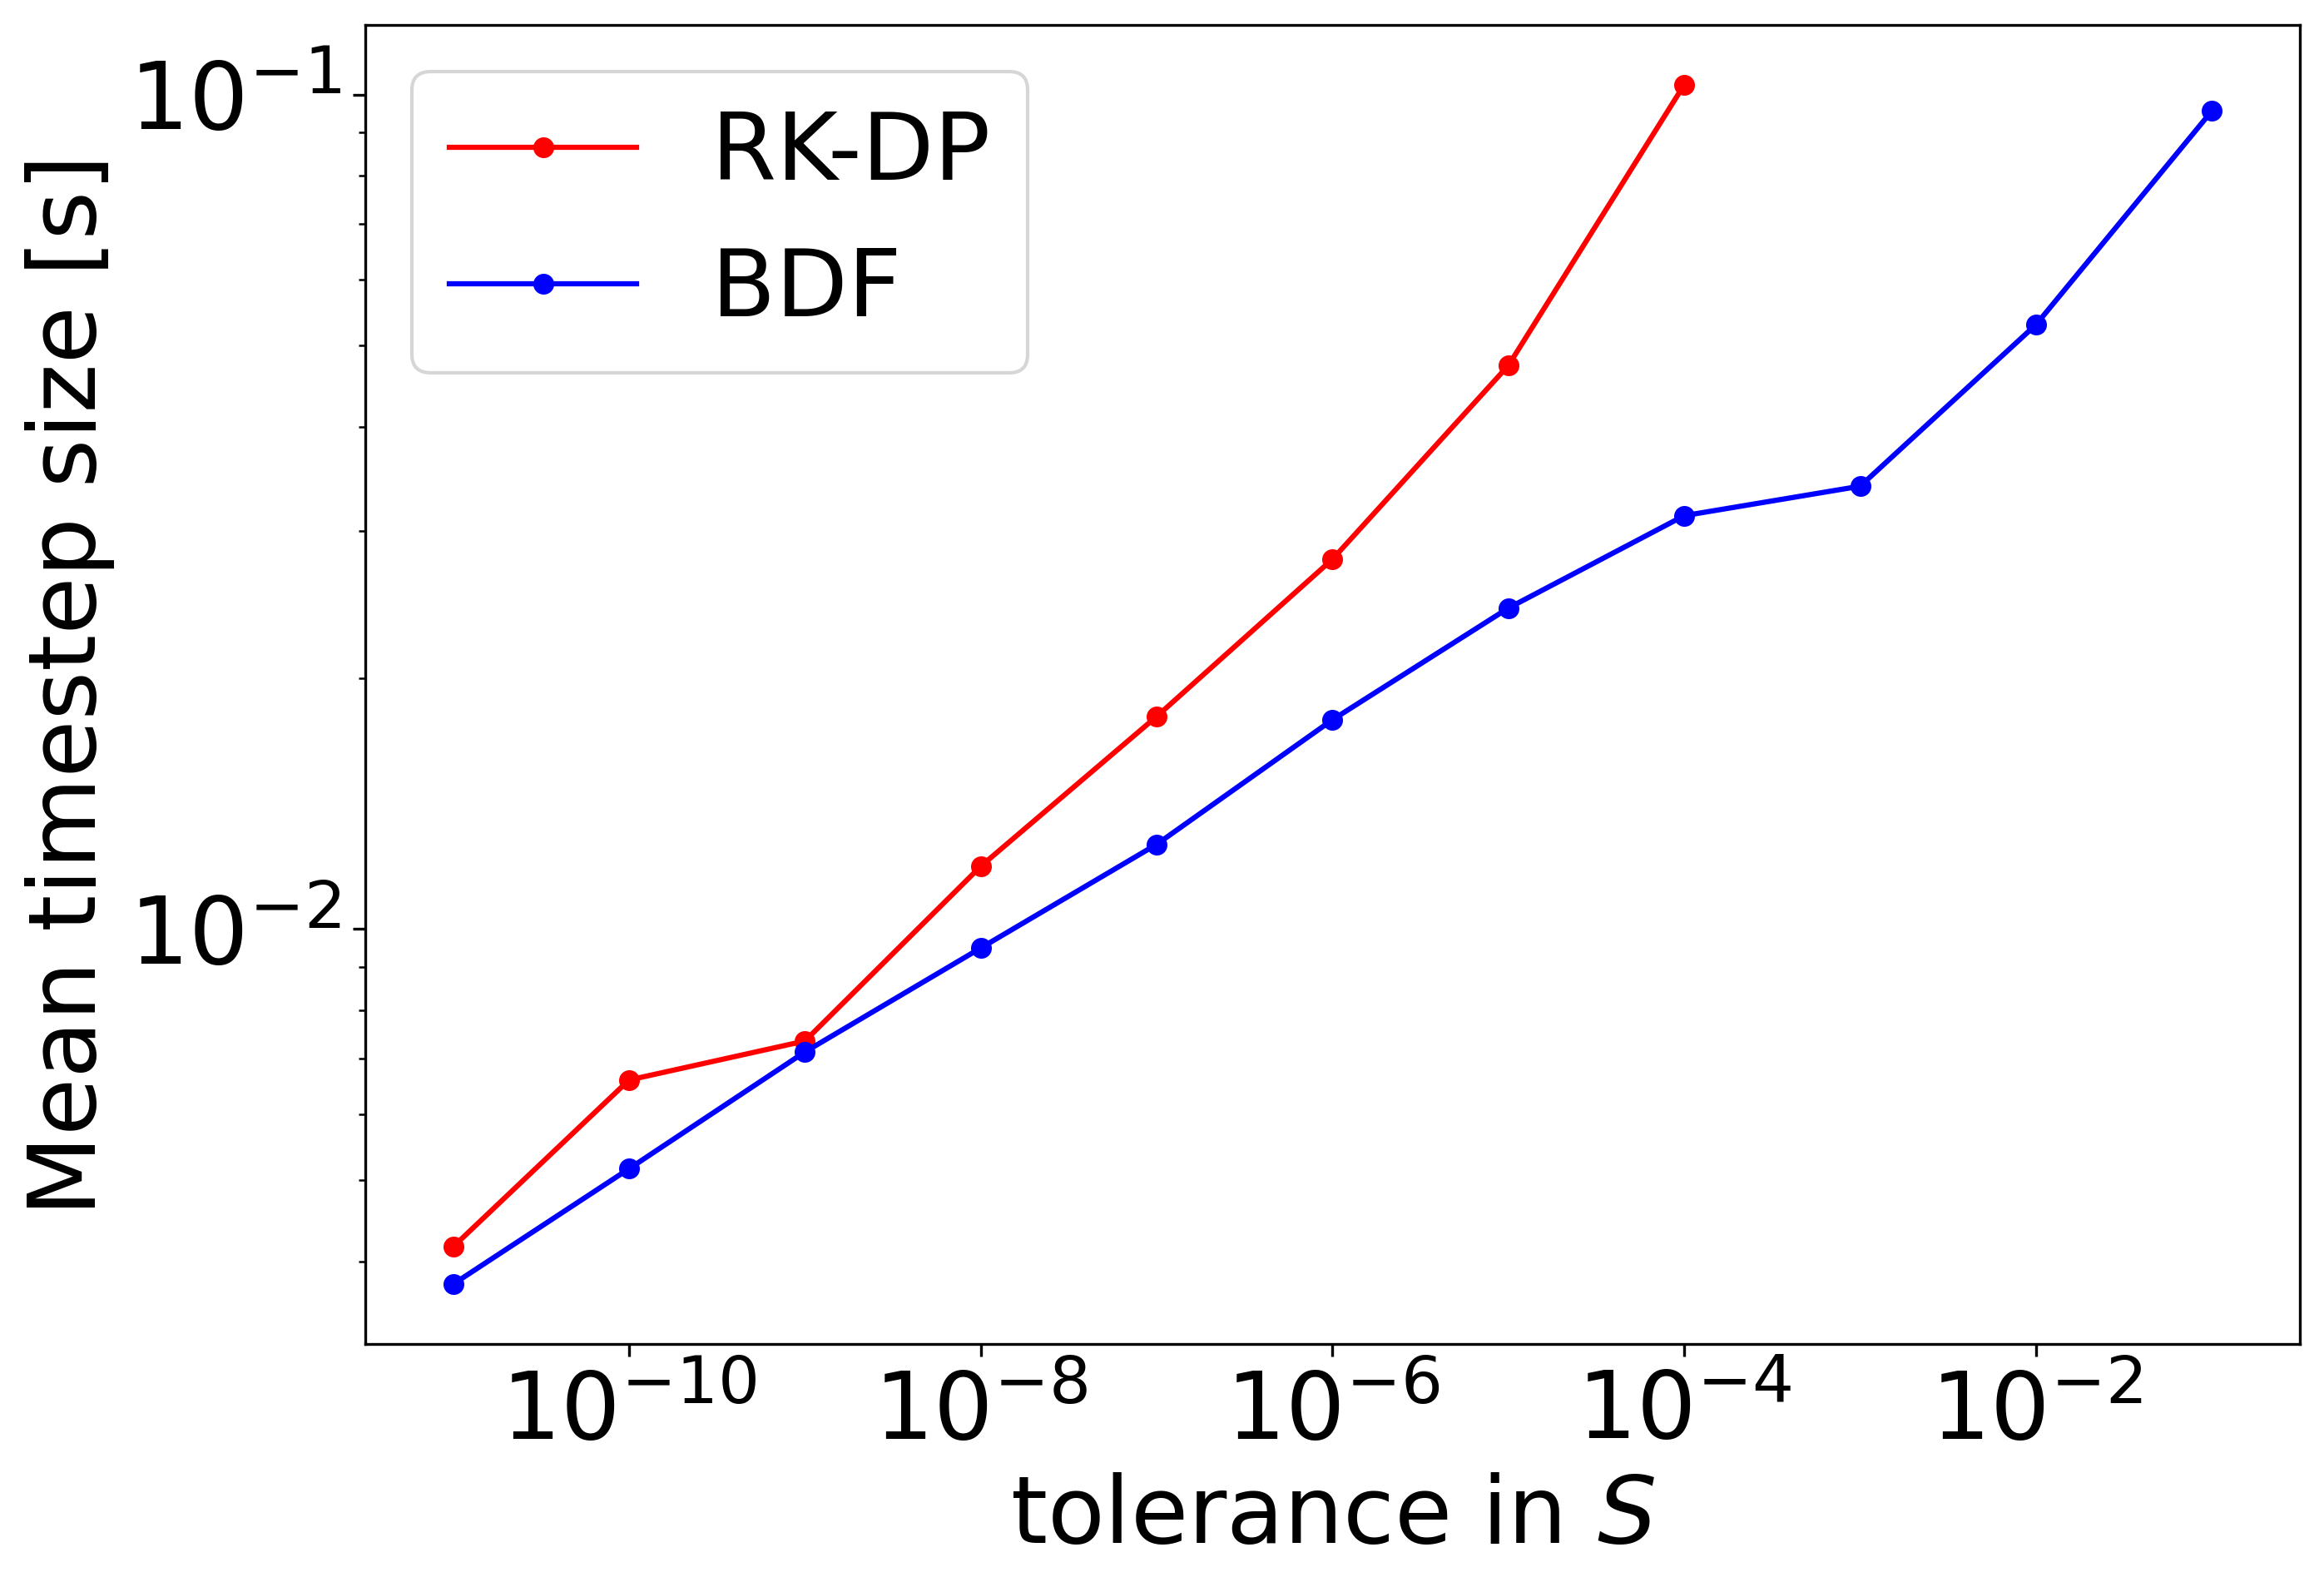
\includegraphics[width=1\textwidth]{images/TANDEMcompactODEDifferentTolerancesSize101_EQ_DT.png}
		\subcaption{Geometric mean of the timestep size in the earthquake} 
	\end{subfigure}
	\caption{Difference of characteristic quantities to the reference solution for different tolerances in the earthquake for a domain with 101 fault elements with the 1st order ODE formulation}
	\label{fig:tolerancesEarthquake_compactODE}
\end{figure}
The slip induced by the earthquake is predicted in general with very high accuracy. Stricter tolerances cannot ameliorate the results as the error for the slip stagnates around $10^{-8}$ with the RK method and around $10^{-7}$ with the BDF method. The fact that the explicit method is more exact than the implicit one is due to the condition of the Newton iteration and has already been discussed in \autoref{ssec:StoppingCriterionNewton}. Only after the RK method fails to converge at $t_a^S = 10^{-3}$, the accuracy begins to deteriorate exponentially with BDF, but even for the last tested tolerance, the difference to the reference solution is of the order of millimeters. Considering that in the reference solution, most of the simulated time is spent in the earthquake, it is strongly recommended to choose a much lower tolerance than for the aseismic slip. One big advantage of implicit methods here is that they return conclusive results even when explicit methods already failed. \\

In both earthquakes and aseismic phases, the timestep size increases logarithmically with the tolerance. With RK-DP, to increase the timestep size by one order of magnitude, the tolerance has to be four orders larger, which reflects the 4th order accuracy of the scheme. Similarly, for the BDF method, the ratio is six to one, which indicates that the order adapter chooses the BDF6 for most of the steps. However, prescribing a lower BDF order would not scale the timesteps faster up, as the adaptive-order finding already optimizes the time-step size. \\

The extended DAE formulation behaves essentially the same as the BDF method in the graphs above, and the compact DAE only for the aseismic slip since it diverges in earthquakes. \\

\subsection{Second order formulation}
The 2nd order ODE formulation differs by the fact that it is driven by the state variable $\psi$ and the slip rate $V$, and the same set of experiments has been repeated, but for varying relative tolerances in $V$. The reference solution is set to $t_r^V=10^{-11}$, the error in the aseismic phase is shown in \autoref{fig:tolerancesAseismicSlip_extendedODE} and in the earthquake in \autoref{fig:tolerancesEarthquake_extendedODE}.
\begin{figure}[H]
	\centering
	\begin{subfigure}[t]{0.32\textwidth}
		\centering
		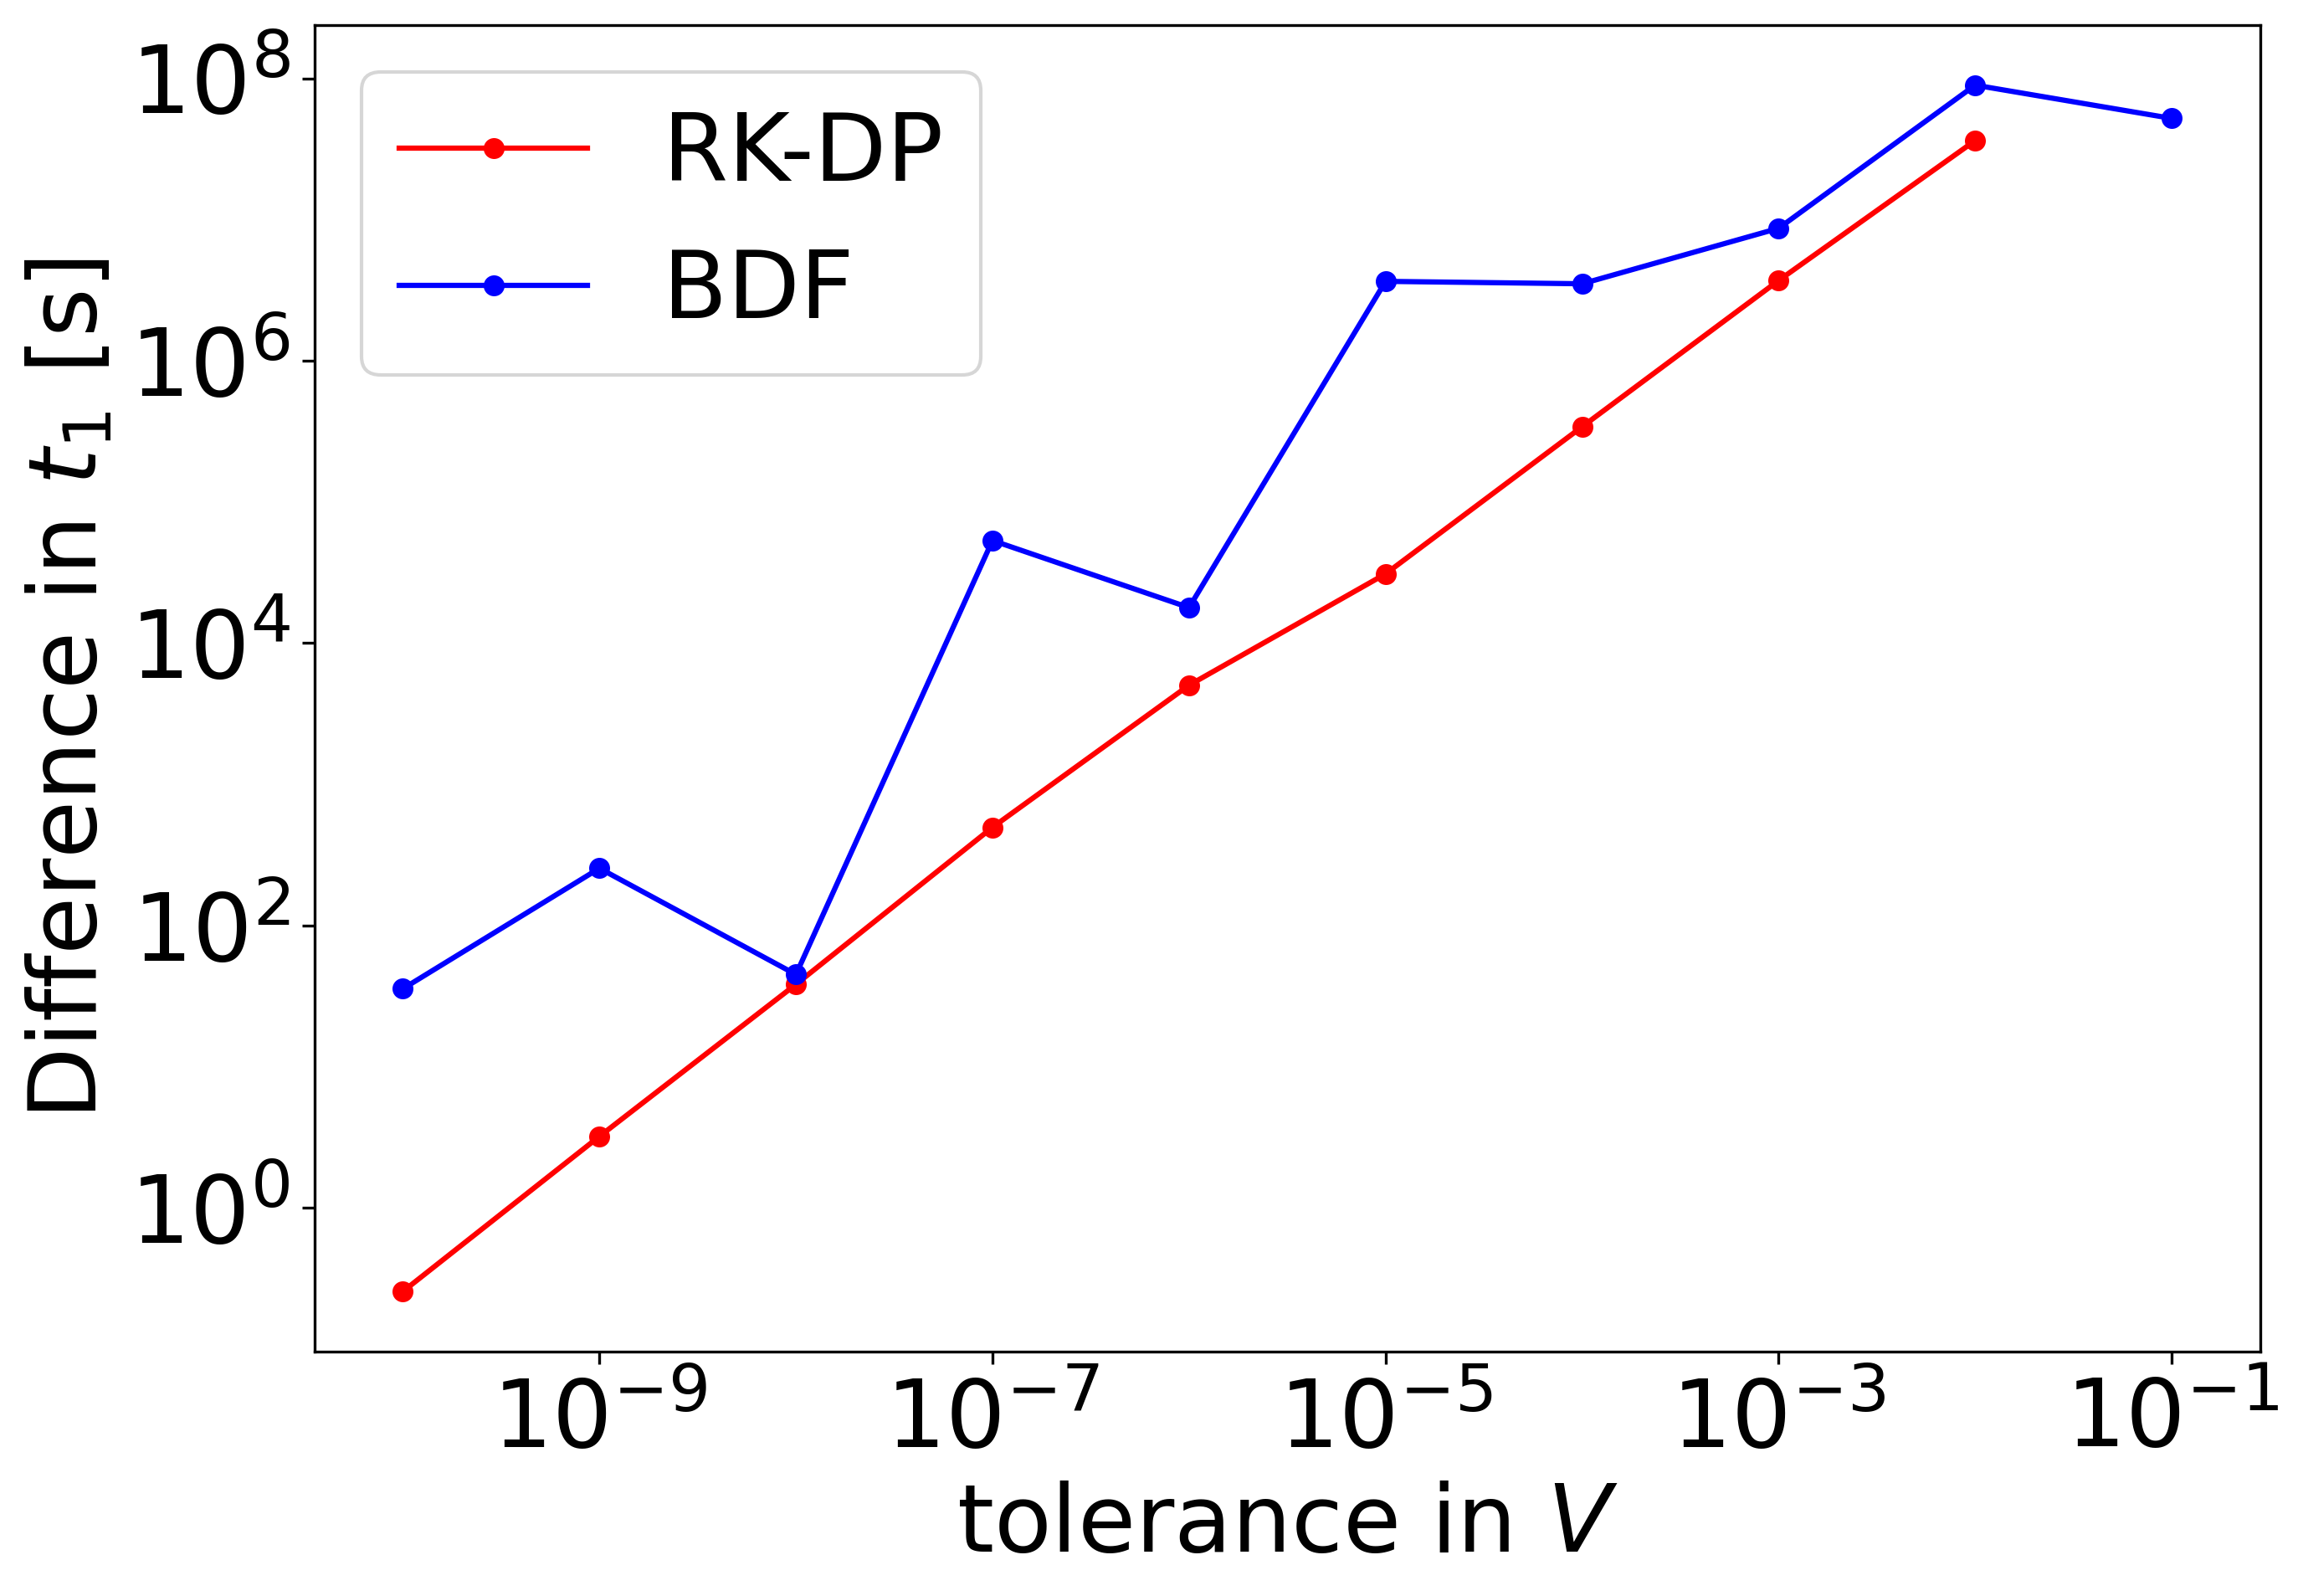
\includegraphics[width=1\textwidth]{images/TANDEMextendedODEDifferentTolerancesSize101_AS_FirstEarthquakeTimeDiff.png}
		\subcaption{Time difference of the first earthquake} 
	\end{subfigure} 
	\begin{subfigure}[t]{0.32\textwidth}
		\centering
		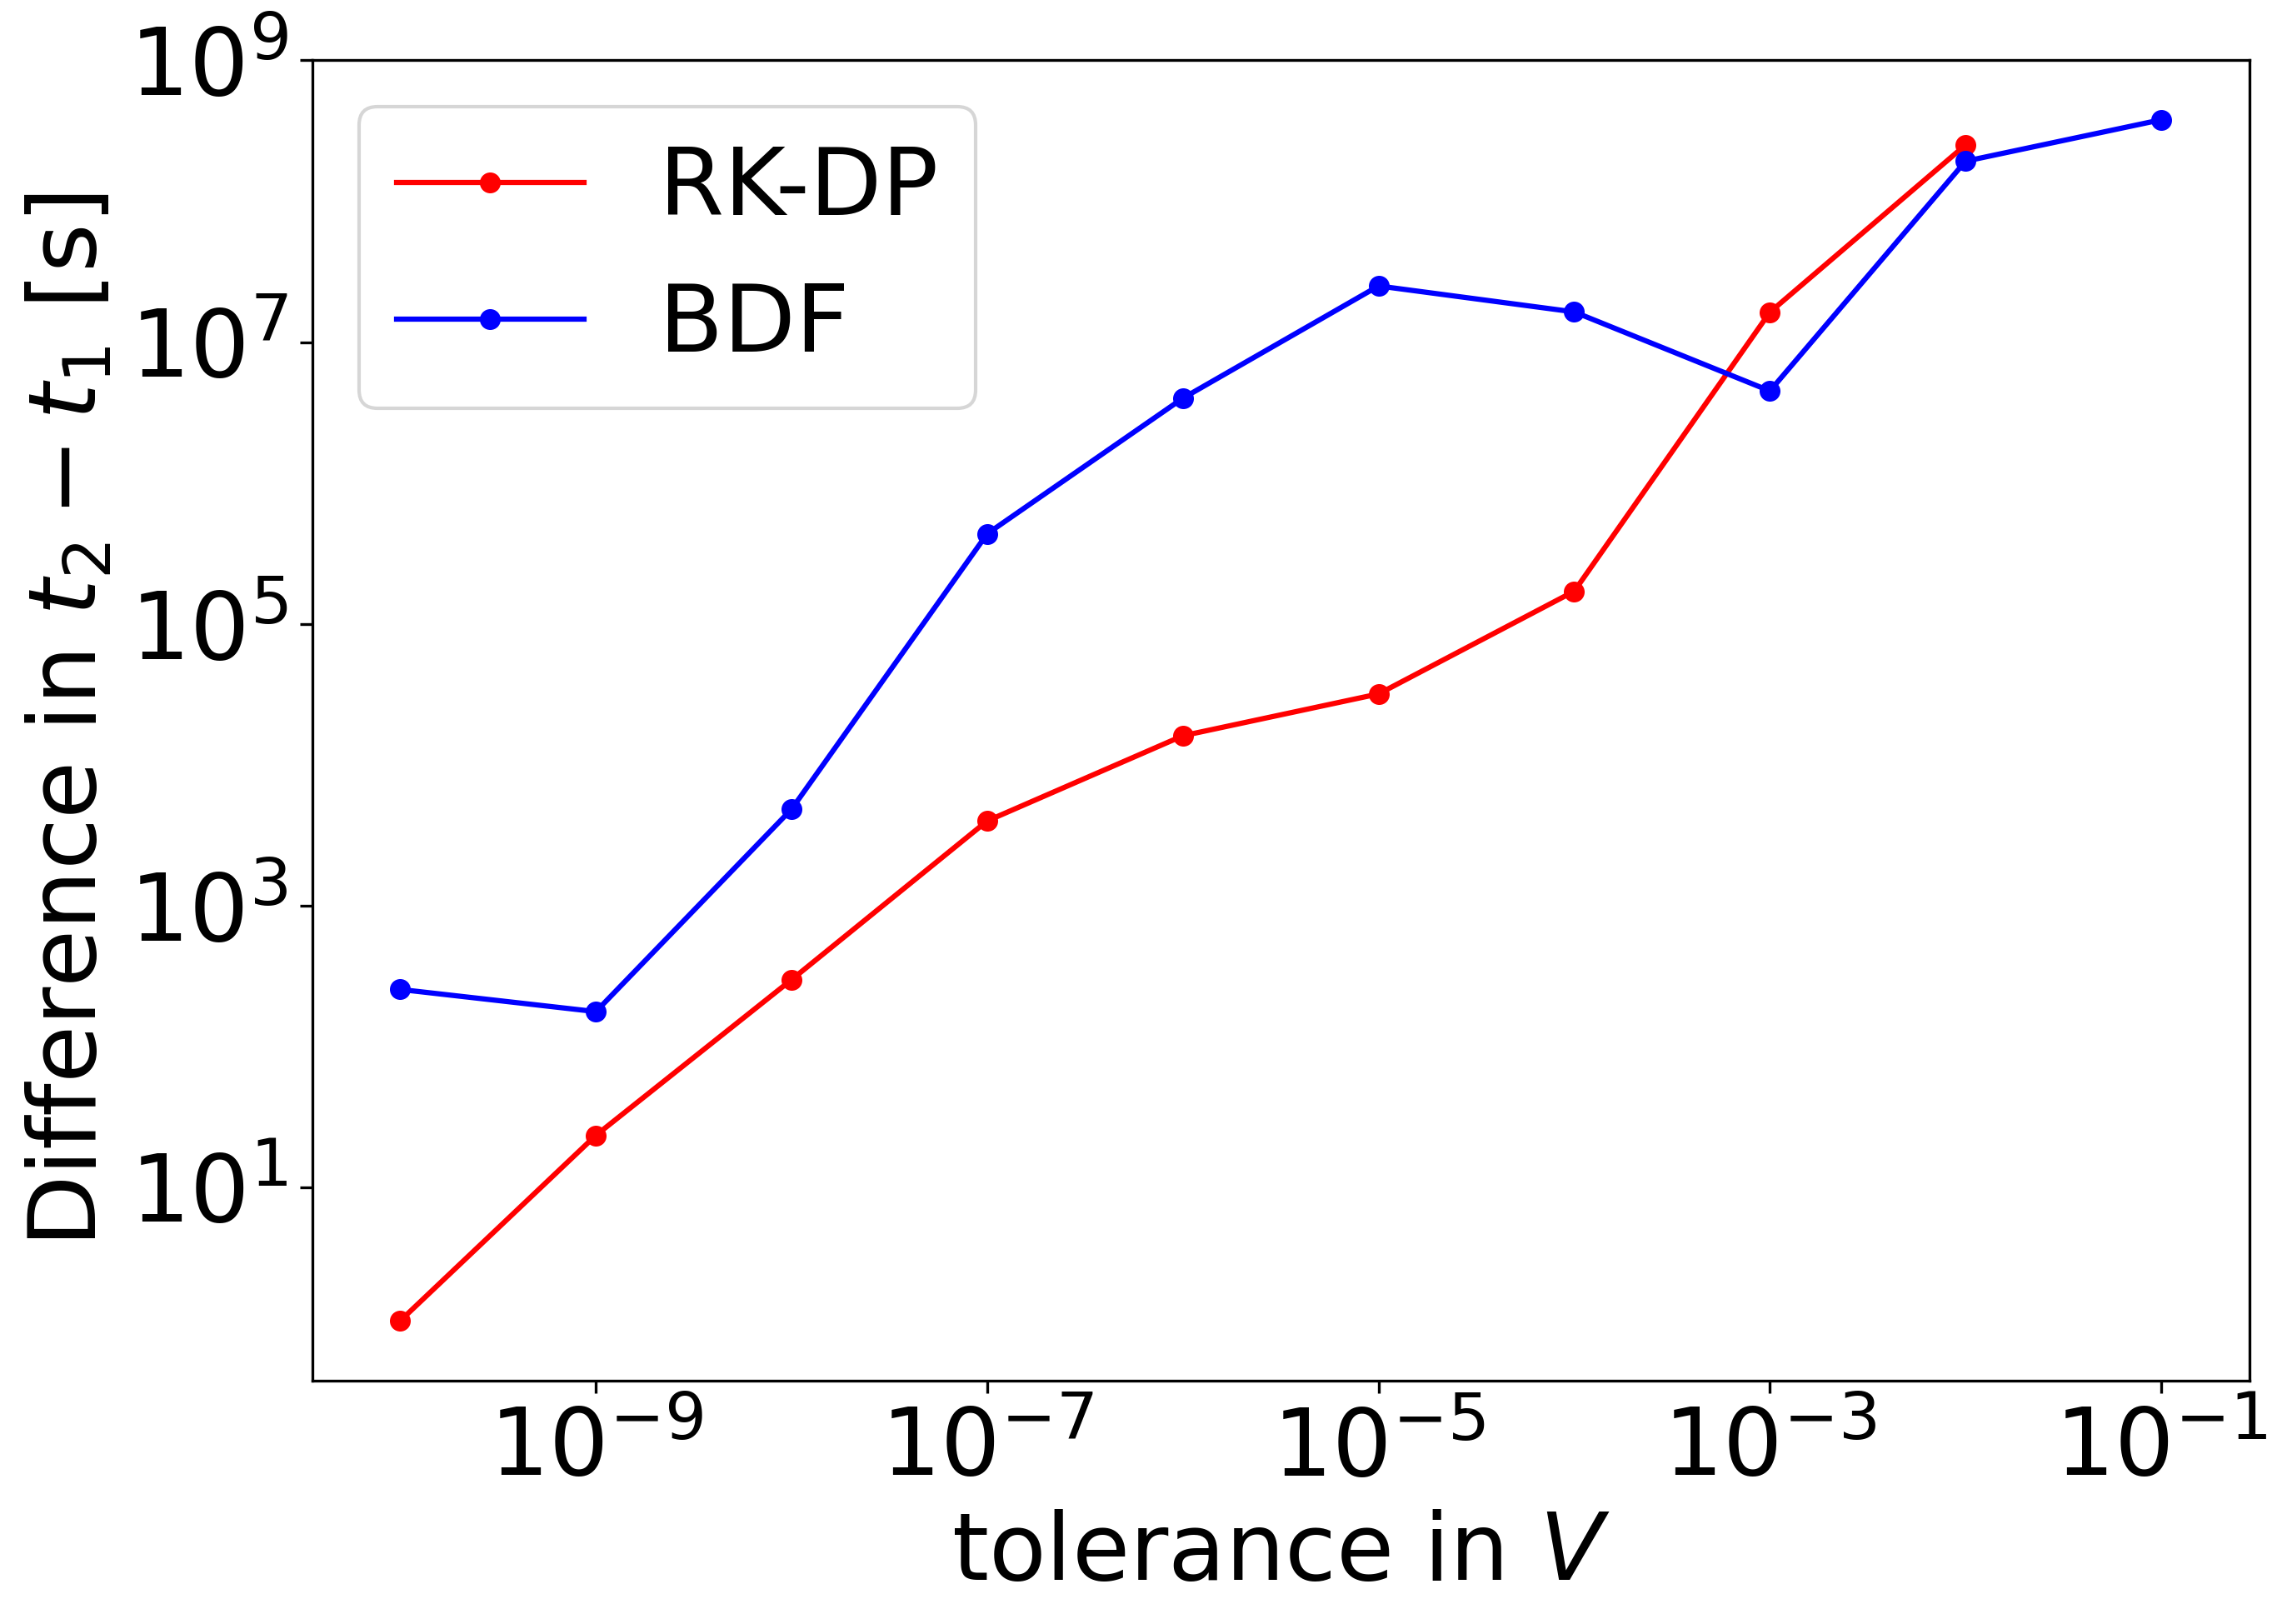
\includegraphics[width=1\textwidth]{images/TANDEMextendedODEDifferentTolerancesSize101_AS_PeriodDiff.png}
		\subcaption{Difference of the period between both earthquakes} 
	\end{subfigure}
	\begin{subfigure}[t]{0.32\textwidth}
		\centering
		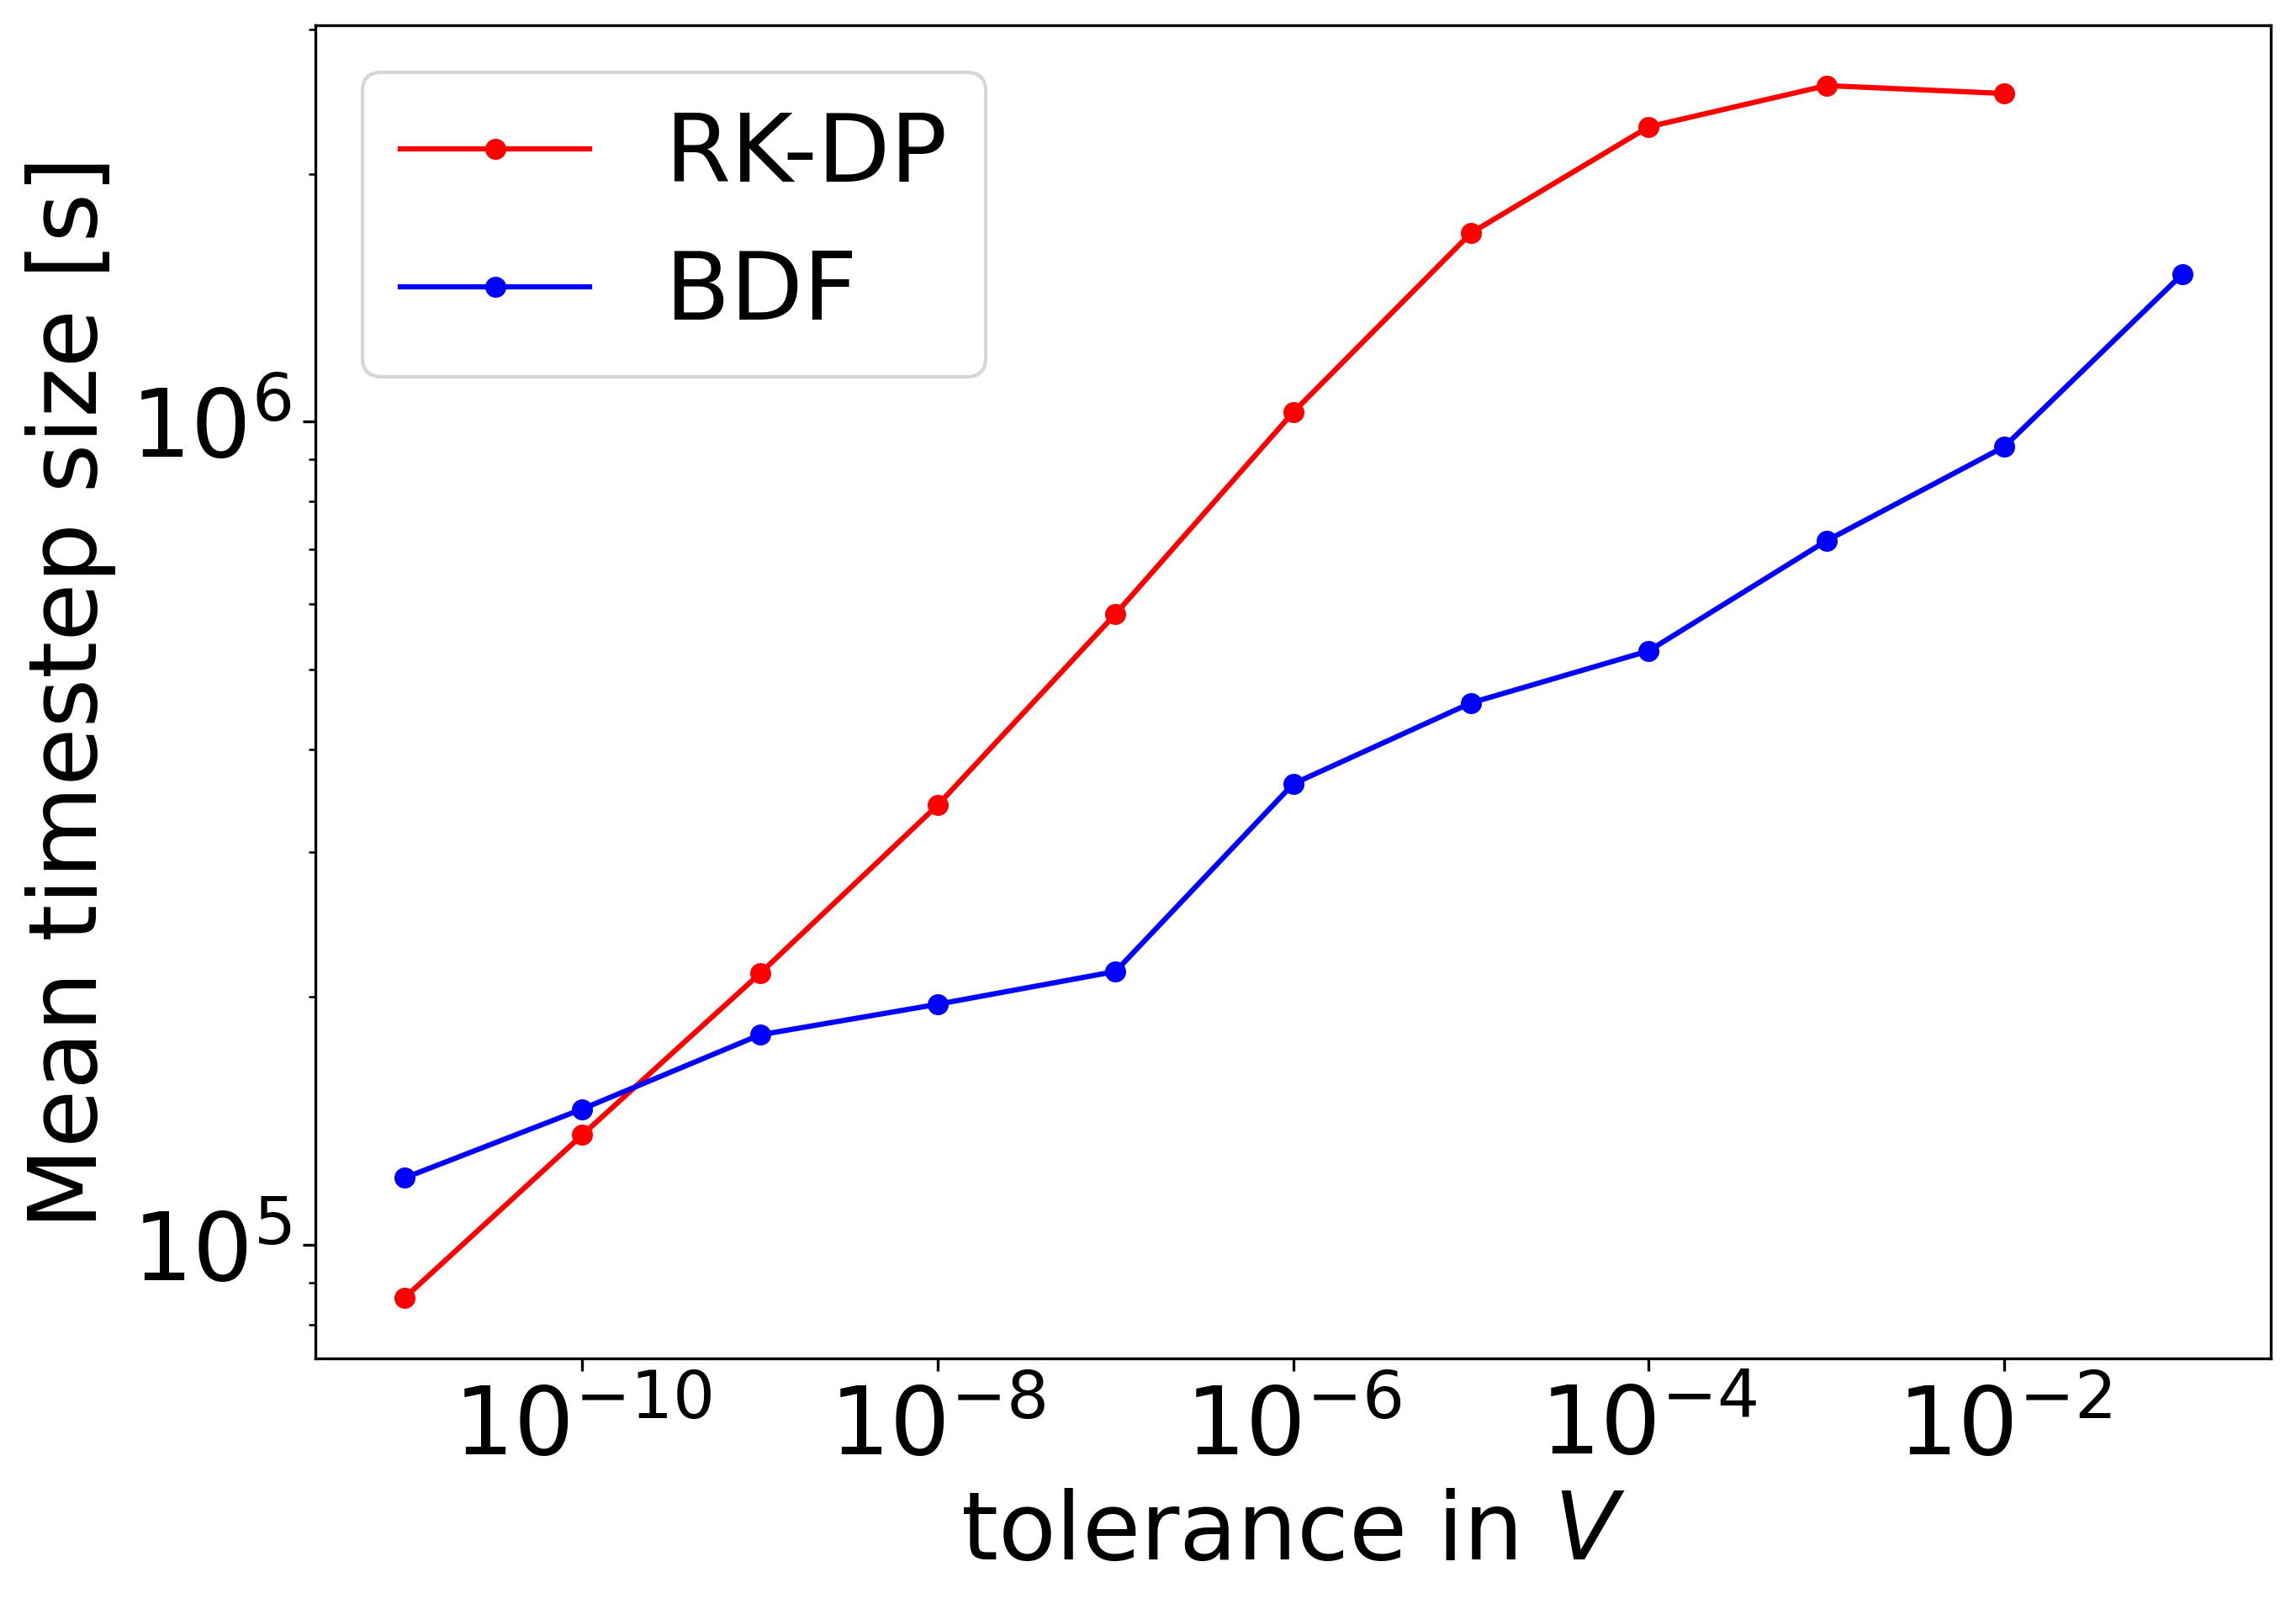
\includegraphics[width=1\textwidth]{images/TANDEMextendedODEDifferentTolerancesSize101_AS_DT.png}
		\subcaption{Geometric mean of the timestep size in the aseismic slip} 
	\end{subfigure}
	\caption{Difference of characteristic times to the reference solution for different tolerances in the aseismic slip phase for a domain with 101 fault elements with the 2nd order ODE formulation}
	\label{fig:tolerancesAseismicSlip_extendedODE}
\end{figure}



\begin{figure}[H]
	\centering
	\begin{subfigure}[t]{0.32\textwidth}
		\centering
		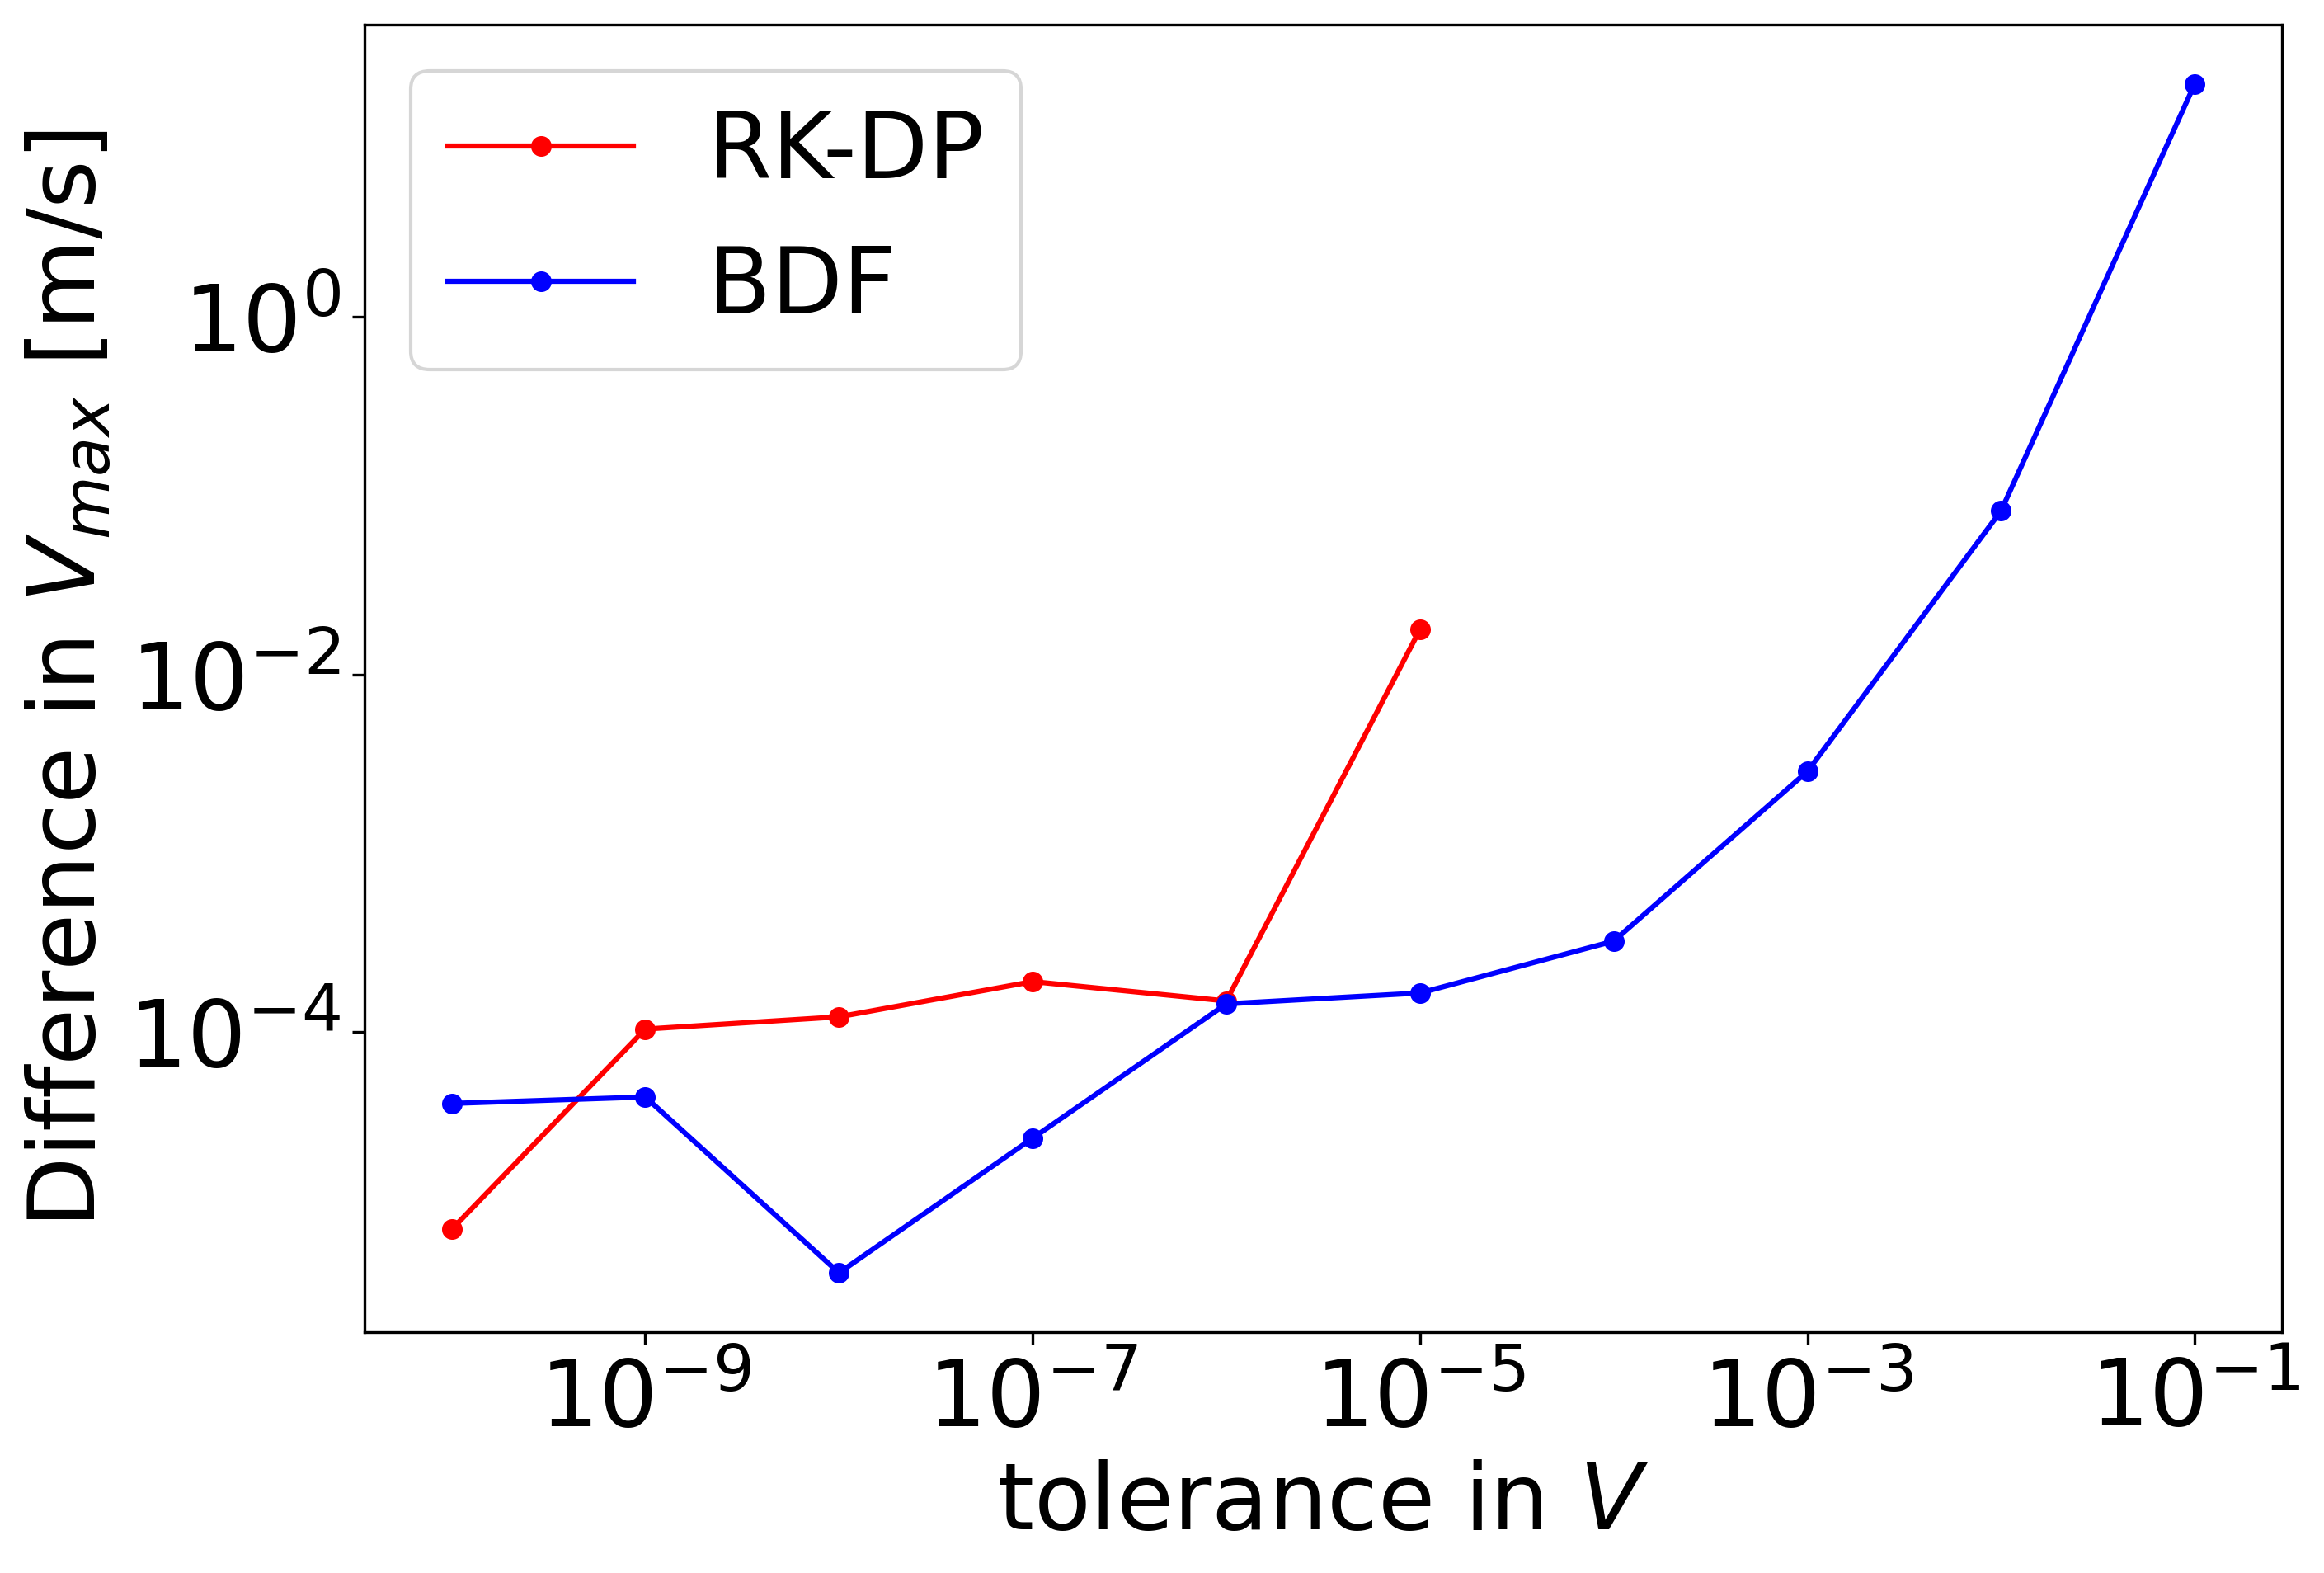
\includegraphics[width=1\textwidth]{images/TANDEMextendedODEDifferentTolerancesSize101_EQ_Vmax.png}
		\subcaption{Difference in the maximum slip rate} 
	\end{subfigure} 
	\begin{subfigure}[t]{0.32\textwidth}
		\centering
		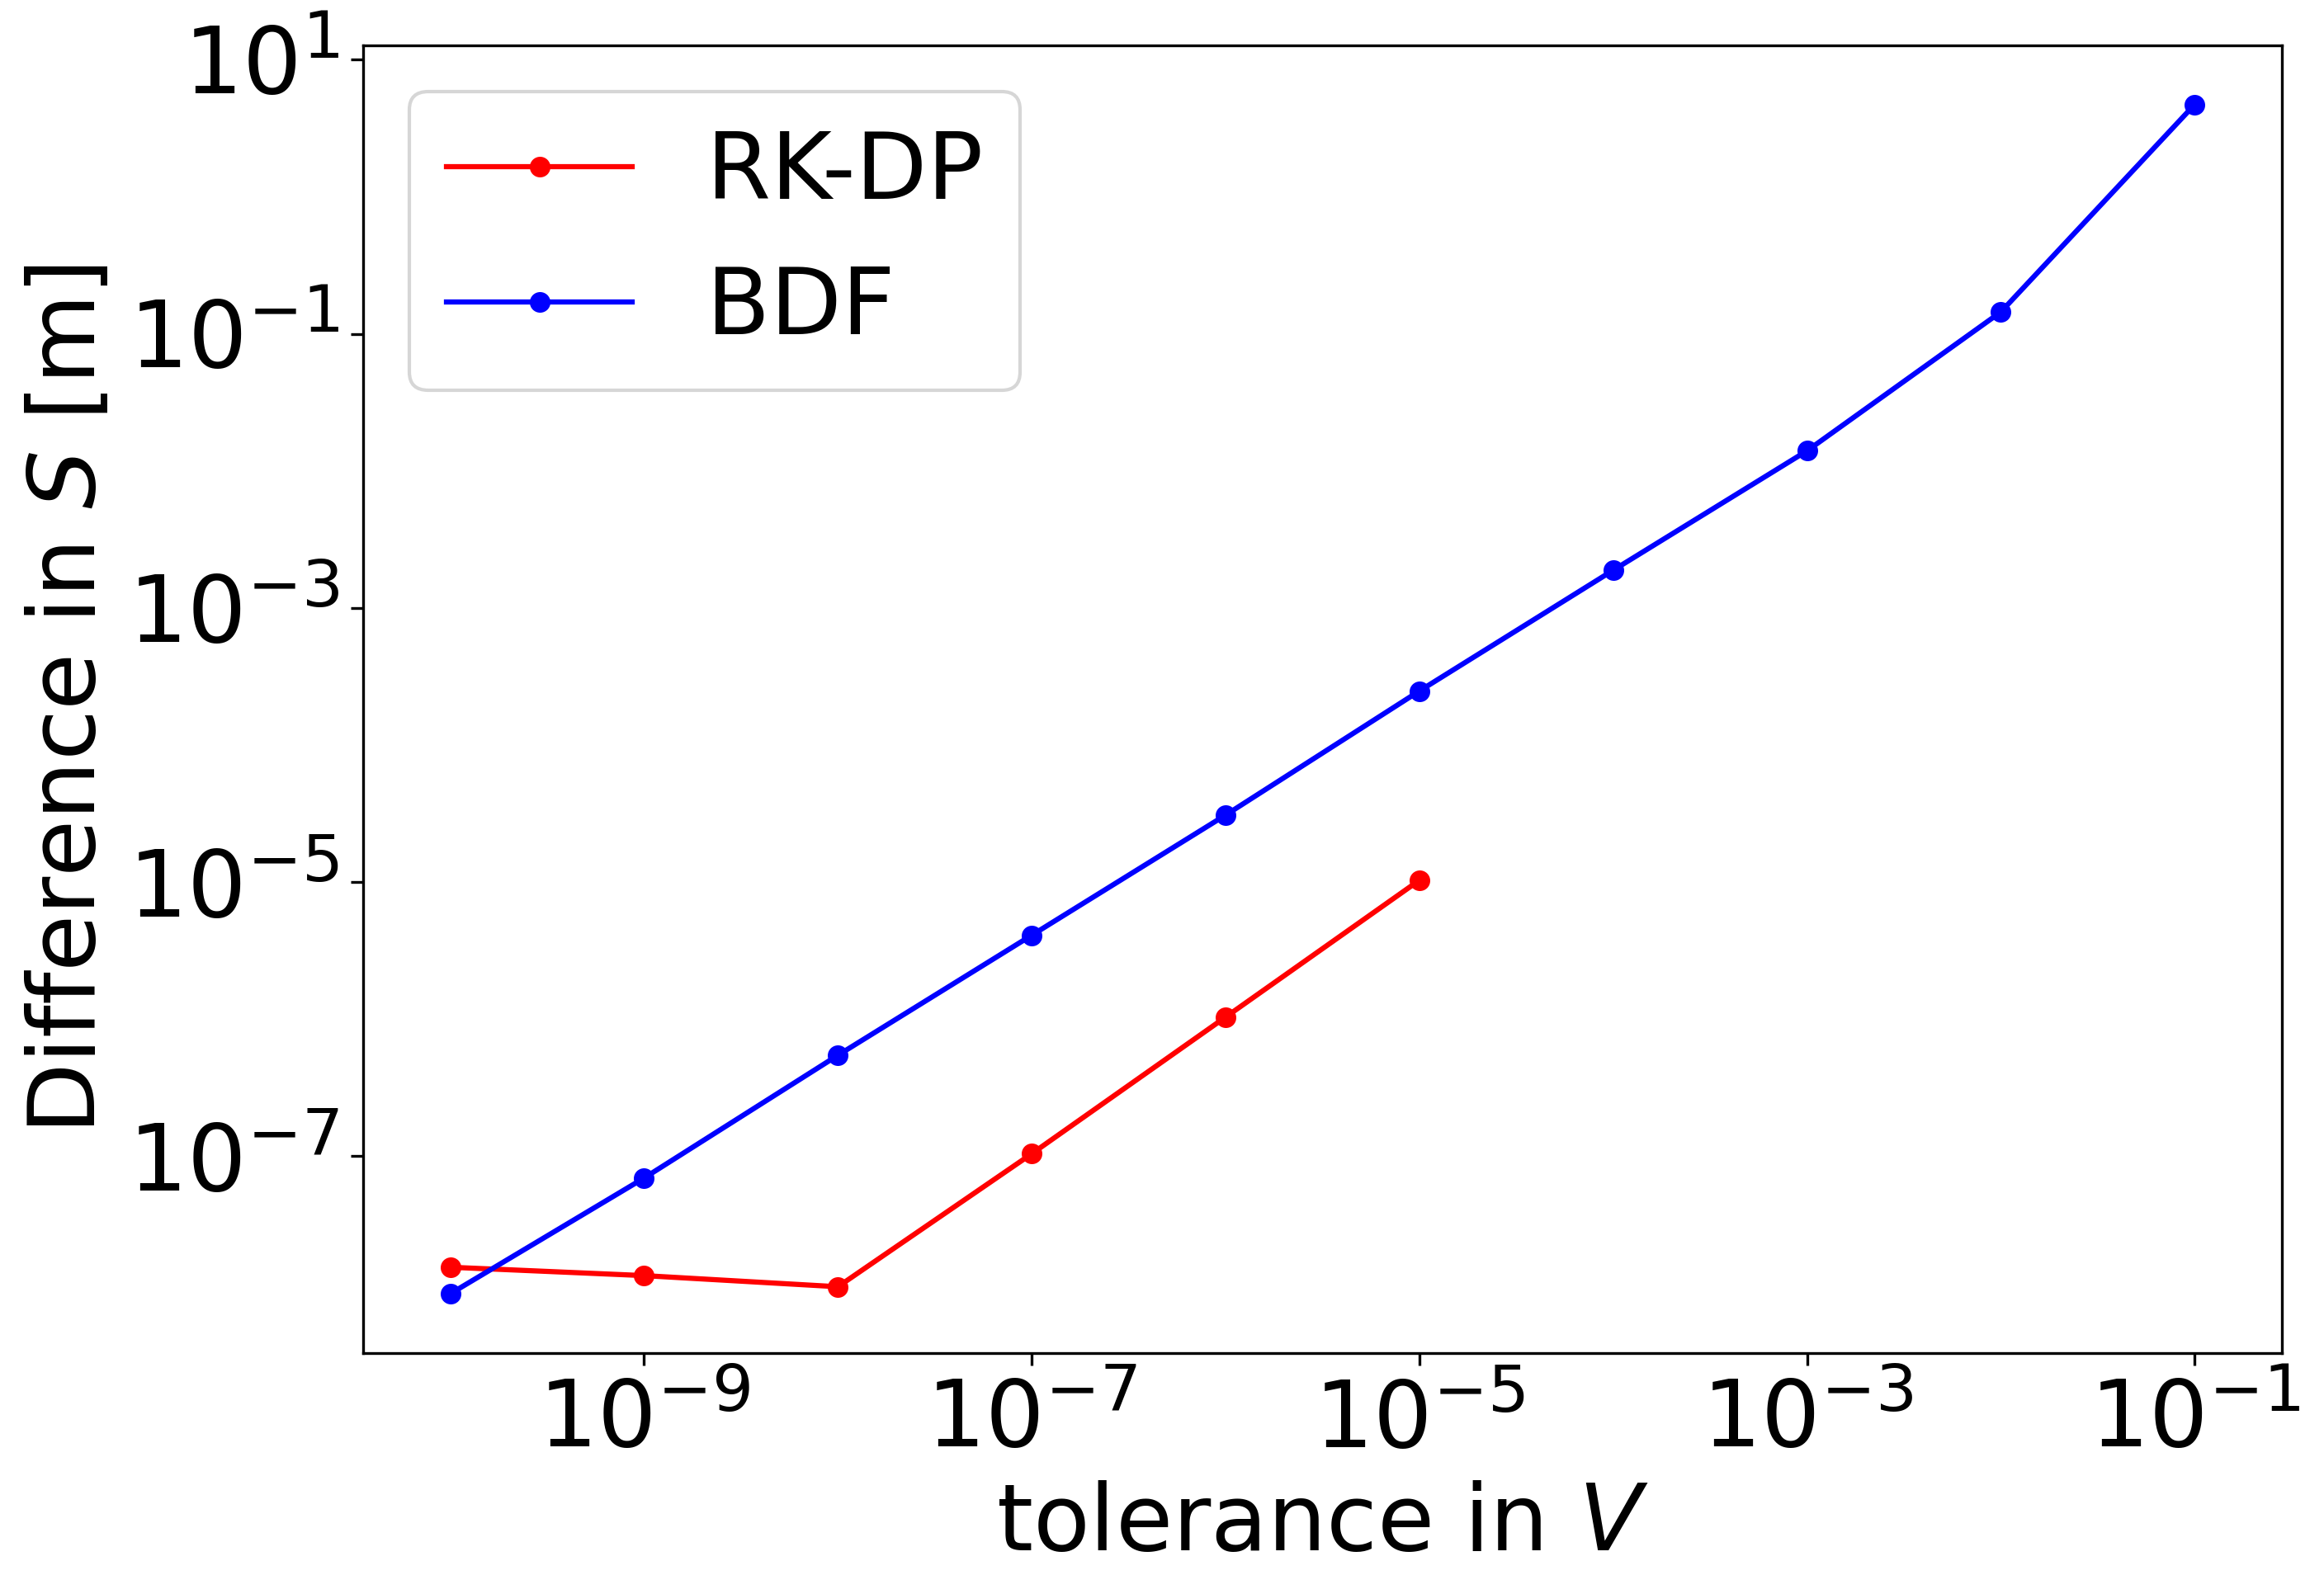
\includegraphics[width=1\textwidth]{images/TANDEMextendedODEDifferentTolerancesSize101_EQ_Smin.png}
		\subcaption{Difference in the slip increase} 
	\end{subfigure}
	\begin{subfigure}[t]{0.32\textwidth}
		\centering
		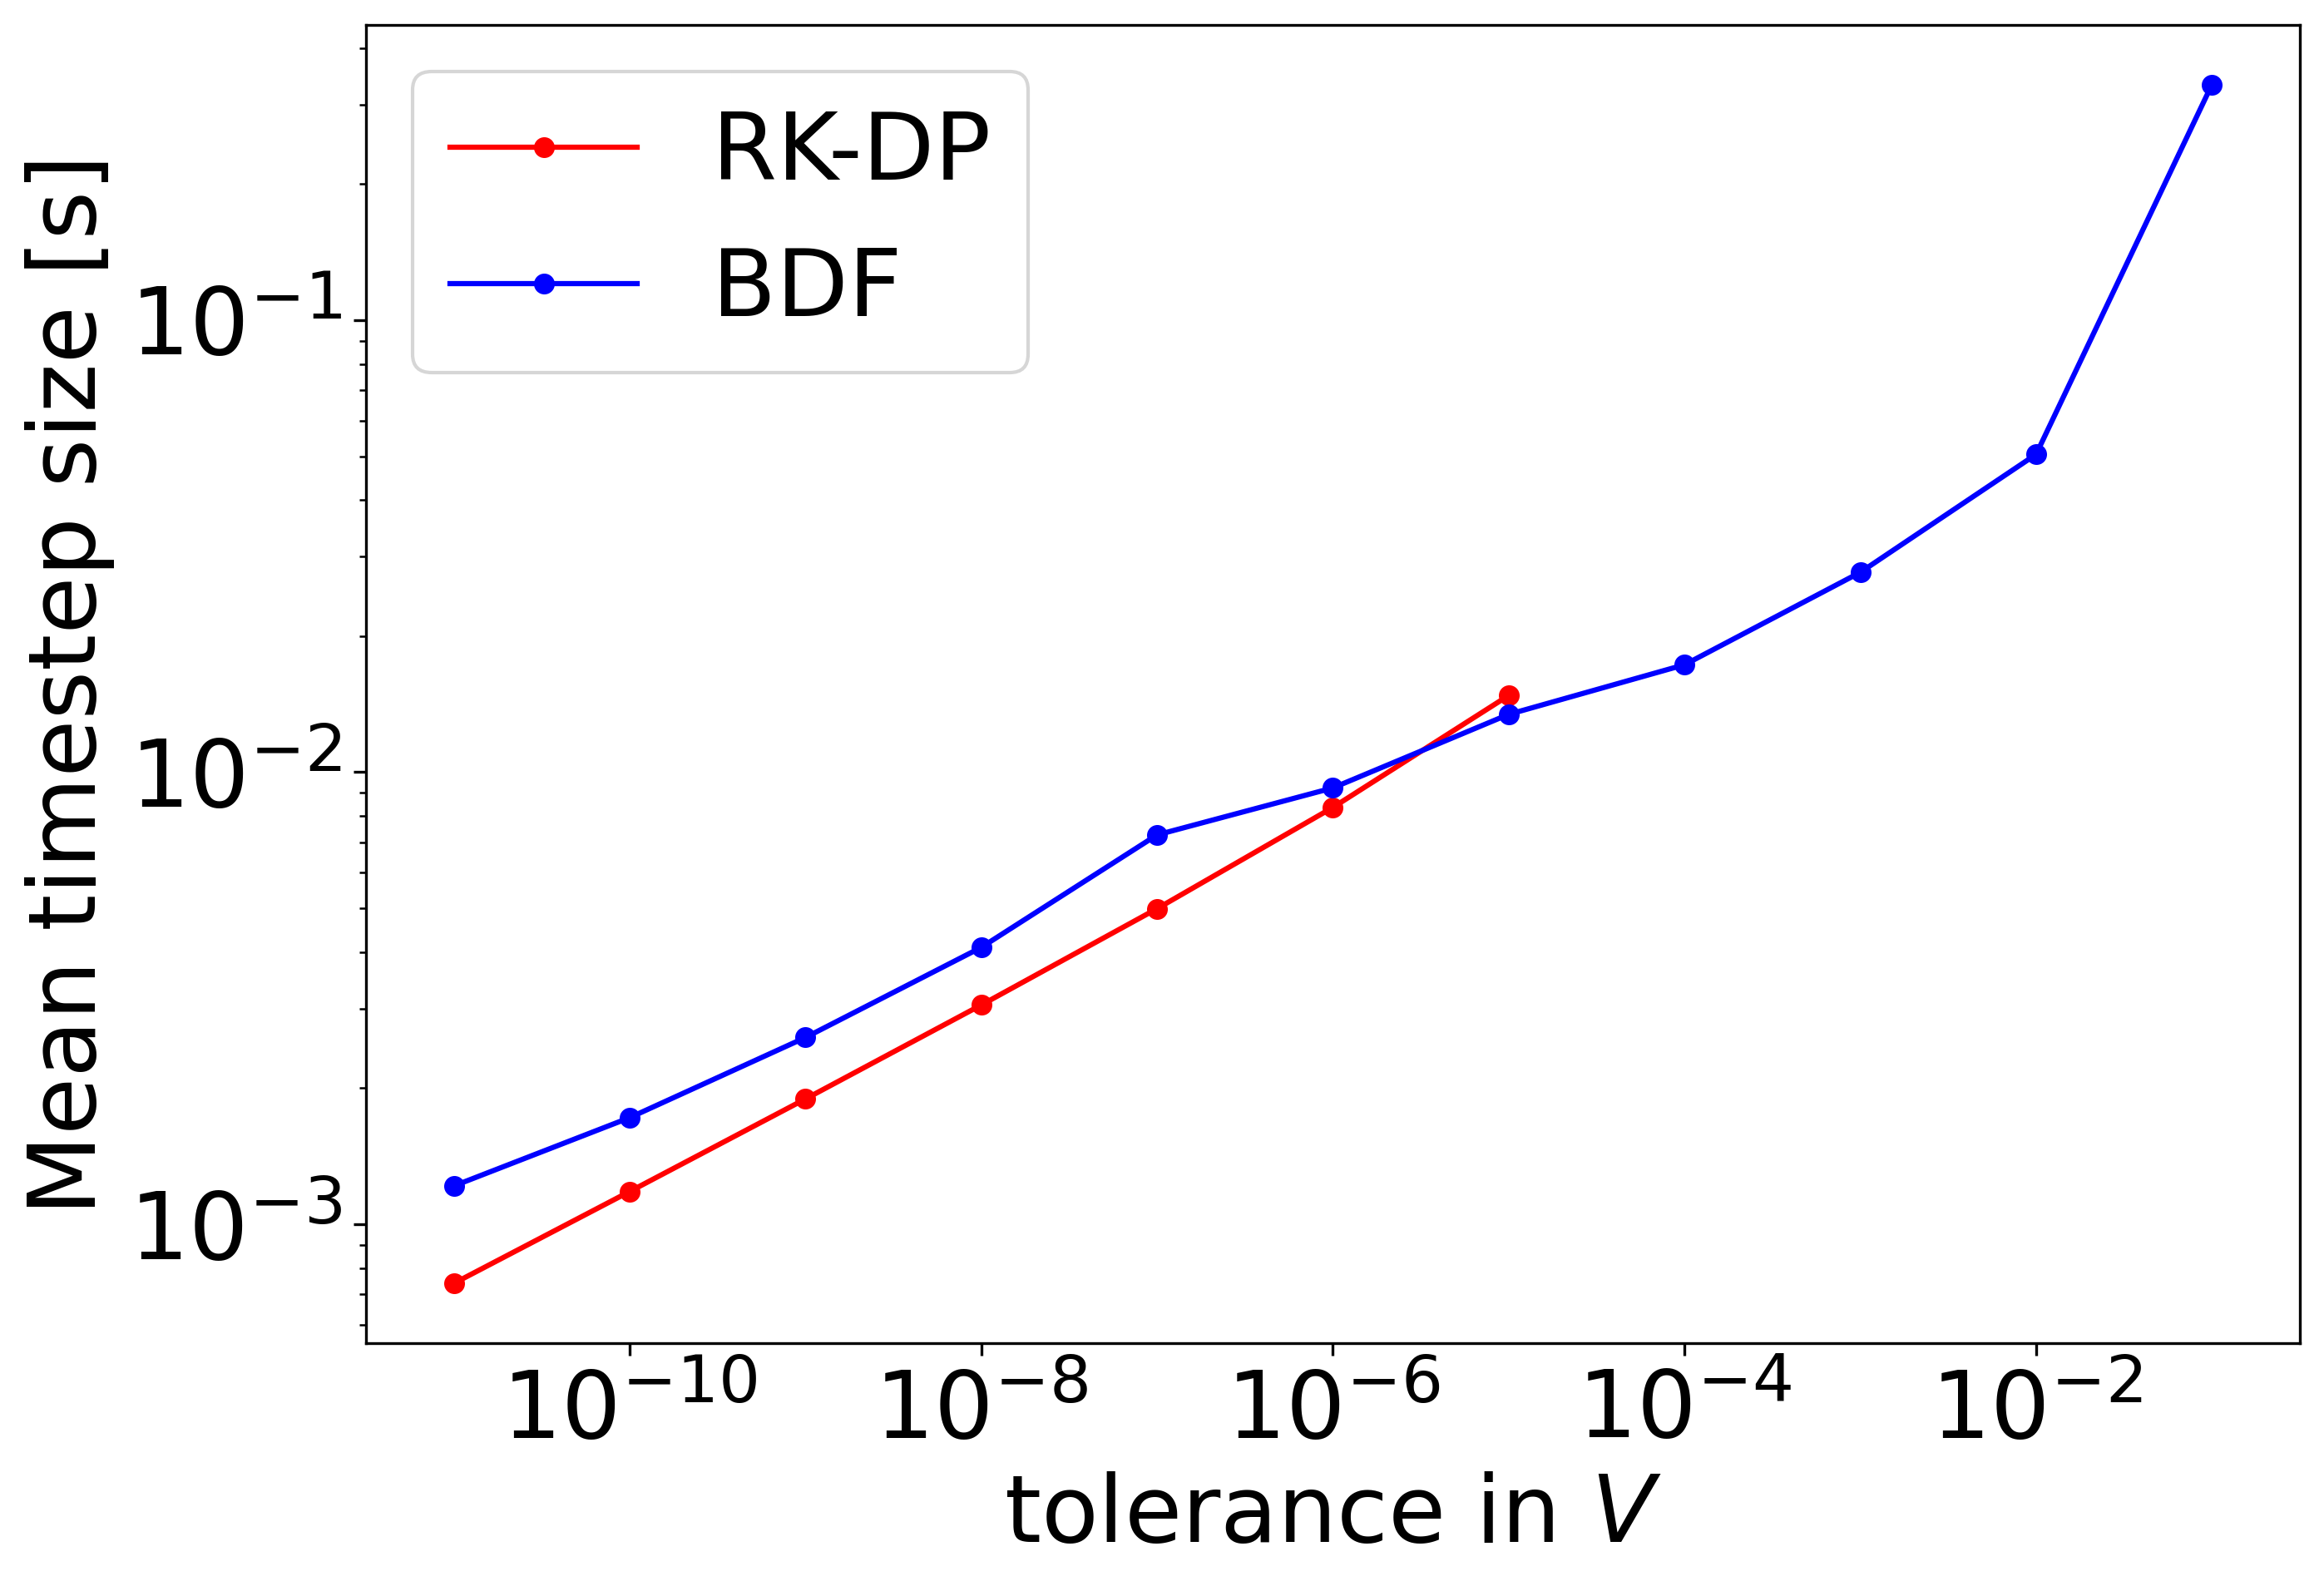
\includegraphics[width=1\textwidth]{images/TANDEMextendedODEDifferentTolerancesSize101_EQ_DT.png}
		\subcaption{Geometric mean of the timestep size in the earthquake} 
	\end{subfigure}
	\caption{Difference of characteristic quantities to the reference solution for different tolerances in the earthquake for a domain with 101 fault elements with the 2nd order ODE formulation}
	\label{fig:tolerancesEarthquake_extendedODE}
\end{figure}

Again, the accuracy increases with smaller tolerances, and the timestep size scales faster for the RK than for the BDF method. The RK method also fails if the tolerance is too large, but instead of NaNs, the slip rate just vanishes and the simulation finishes without detecting any earthquakes. Unlike the first order formulations, the second order ODE comes along with a much more accurate error estimate which is discussed in detail in the next section.




\section{Error estimation of the 2nd order ODE formulation}
\label{sec:Results_ErrorEstimate2ndOrderODE}
Despite the lack of an analytic solution to the problem, the second order ODE formulation of the problem offers a very powerful tool to evaluate the accuracy of the results. Since the slip rate is not calculated from the friction law anymore, it is not ensured that it is always equal to 0 up to numerical precision, as it was the case in the first order formulations of the SEAS problem. We could then evaluate the friction law at every timestep to assess the accuracy of the numerical integration. A large deviation from 0 of the absolute value of the friction law at a given timestep means that the formulation provides poor results. For a standard execution of the simulation with the second order formulation, this metric is not available, since the evaluation of $\tau$ in the friction law requires solving the Poisson problem, and the big advantage of the new formulation is exactly not to solve this system. For the following graphs, the residual value of the friction law has been additionally calculated. \\

In the first order formulations, the slip rate is calculated iteratively such that the residual of the friction law is always below a tolerance value, usually $10^{-12}$. This is not true for the second order formulation and the residual increases with each performed timestep. To quantify this increase, a longer simulated time of 400 years has been chosen during which several earthquakes are registered. As previously, the absolute tolerance for the slip rate and all tolerances for the slip and the state variable are set to 0.

\autoref{fig:timeEvolution_2ndOrderODE_differentTolerances} shows the maximum value of the residual for varying relative tolerances for $V$. From the initial condition, the slip rate is calculated to fulfill the friction law up to numerical precision, at about $10^{-15}$. After some timesteps, this high precision is lost, and at every earthquake event, the difference increases sharply. Overall, the logarithmic shape of the curves indicates a linear decrease of accuracy with time. It seems that at every evaluation of the right-hand side a certain local truncation error is added to the residual of the friction law. During an earthquake, much more timesteps are required and the sum of the local truncation errors sum up to form an apparent sharp increase in the global error. Naturally, for lower relative tolerances, the additional error at each timestep is smaller and the global accuracy is higher. The relation seems to depend linear, as a 10 times larger tolerance produces a 10 times larger global residual error. A similar dependency is to be expected with respect to the tolerances of the slip $S$ and $\psi$ since they are directly needed to evaluate the friction law, but it is impossible to know it for sure, since no analytic solution is known for any of these quantities.

\begin{figure}[H]
	\centering
	\begin{subfigure}{0.45\textwidth}
		\centering
		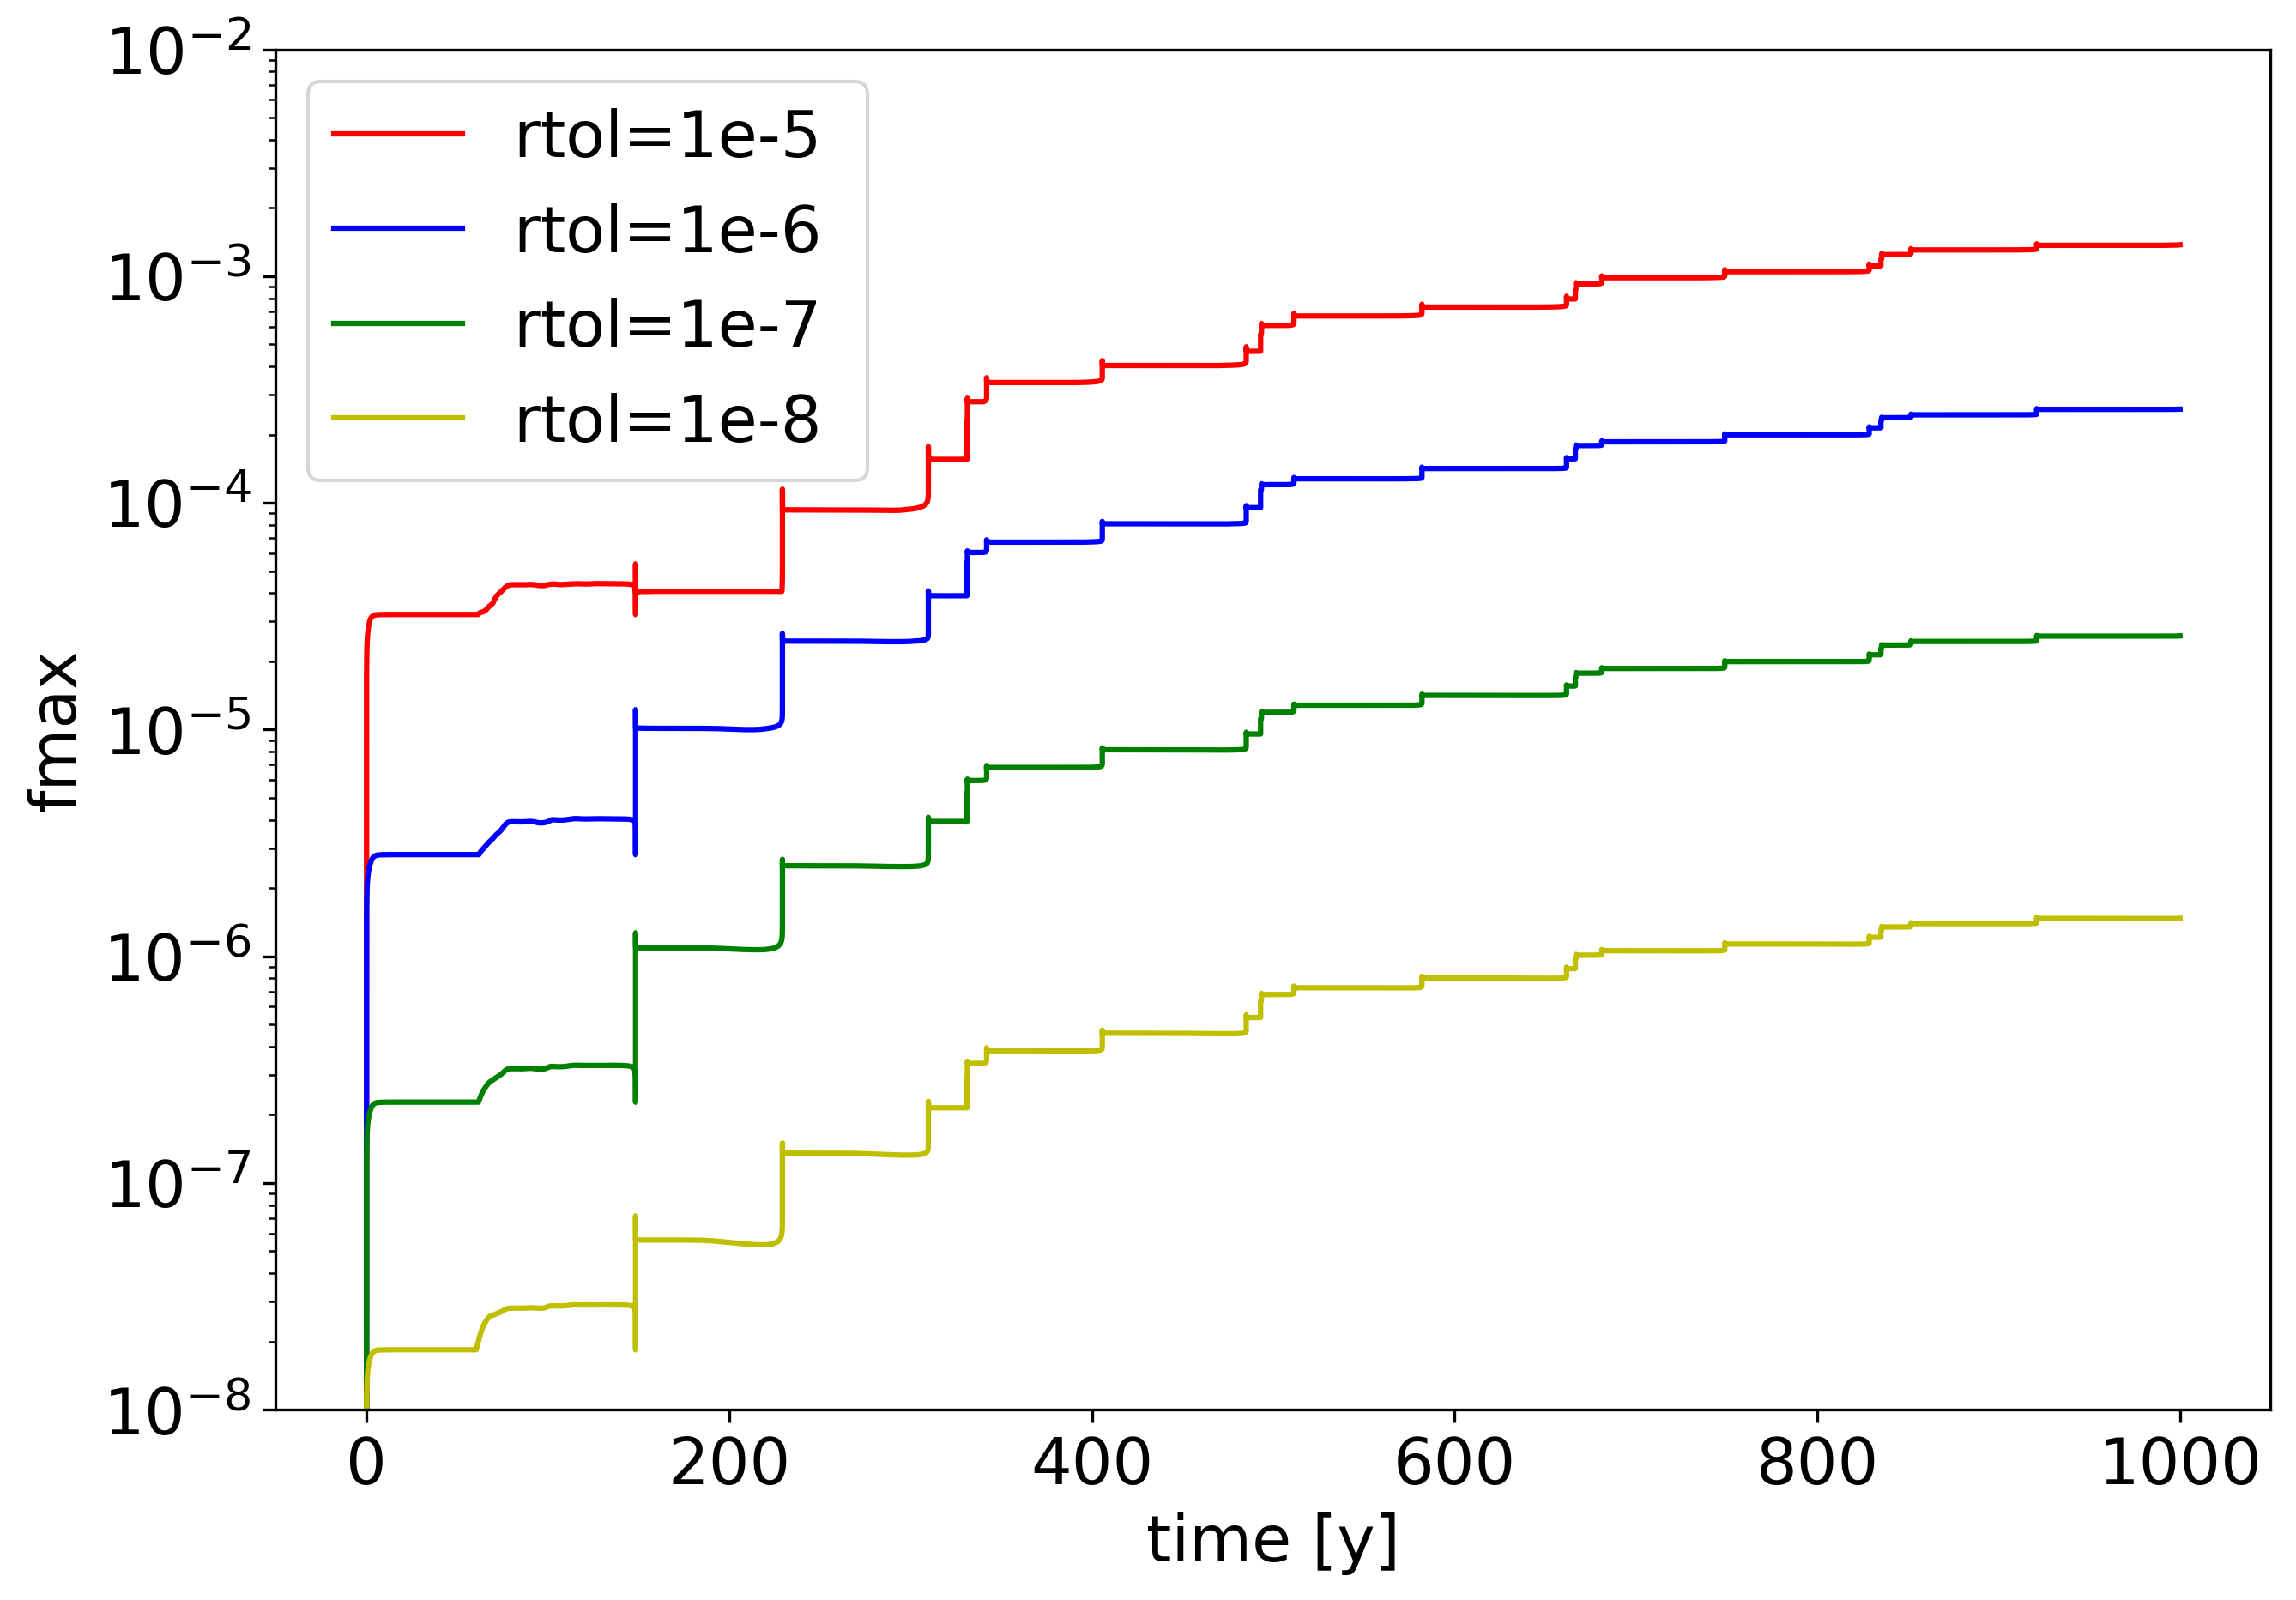
\includegraphics[width=1\textwidth]{images/TANDEMtimeEvolutionFExtendedODEDifferentTolerances.png}
		\subcaption{Fixed mesh resolution with 101 fault elements} 
		\label{fig:timeEvolution_2ndOrderODE_differentTolerances}
	\end{subfigure}
	\begin{subfigure}{0.45\textwidth}
		\centering
		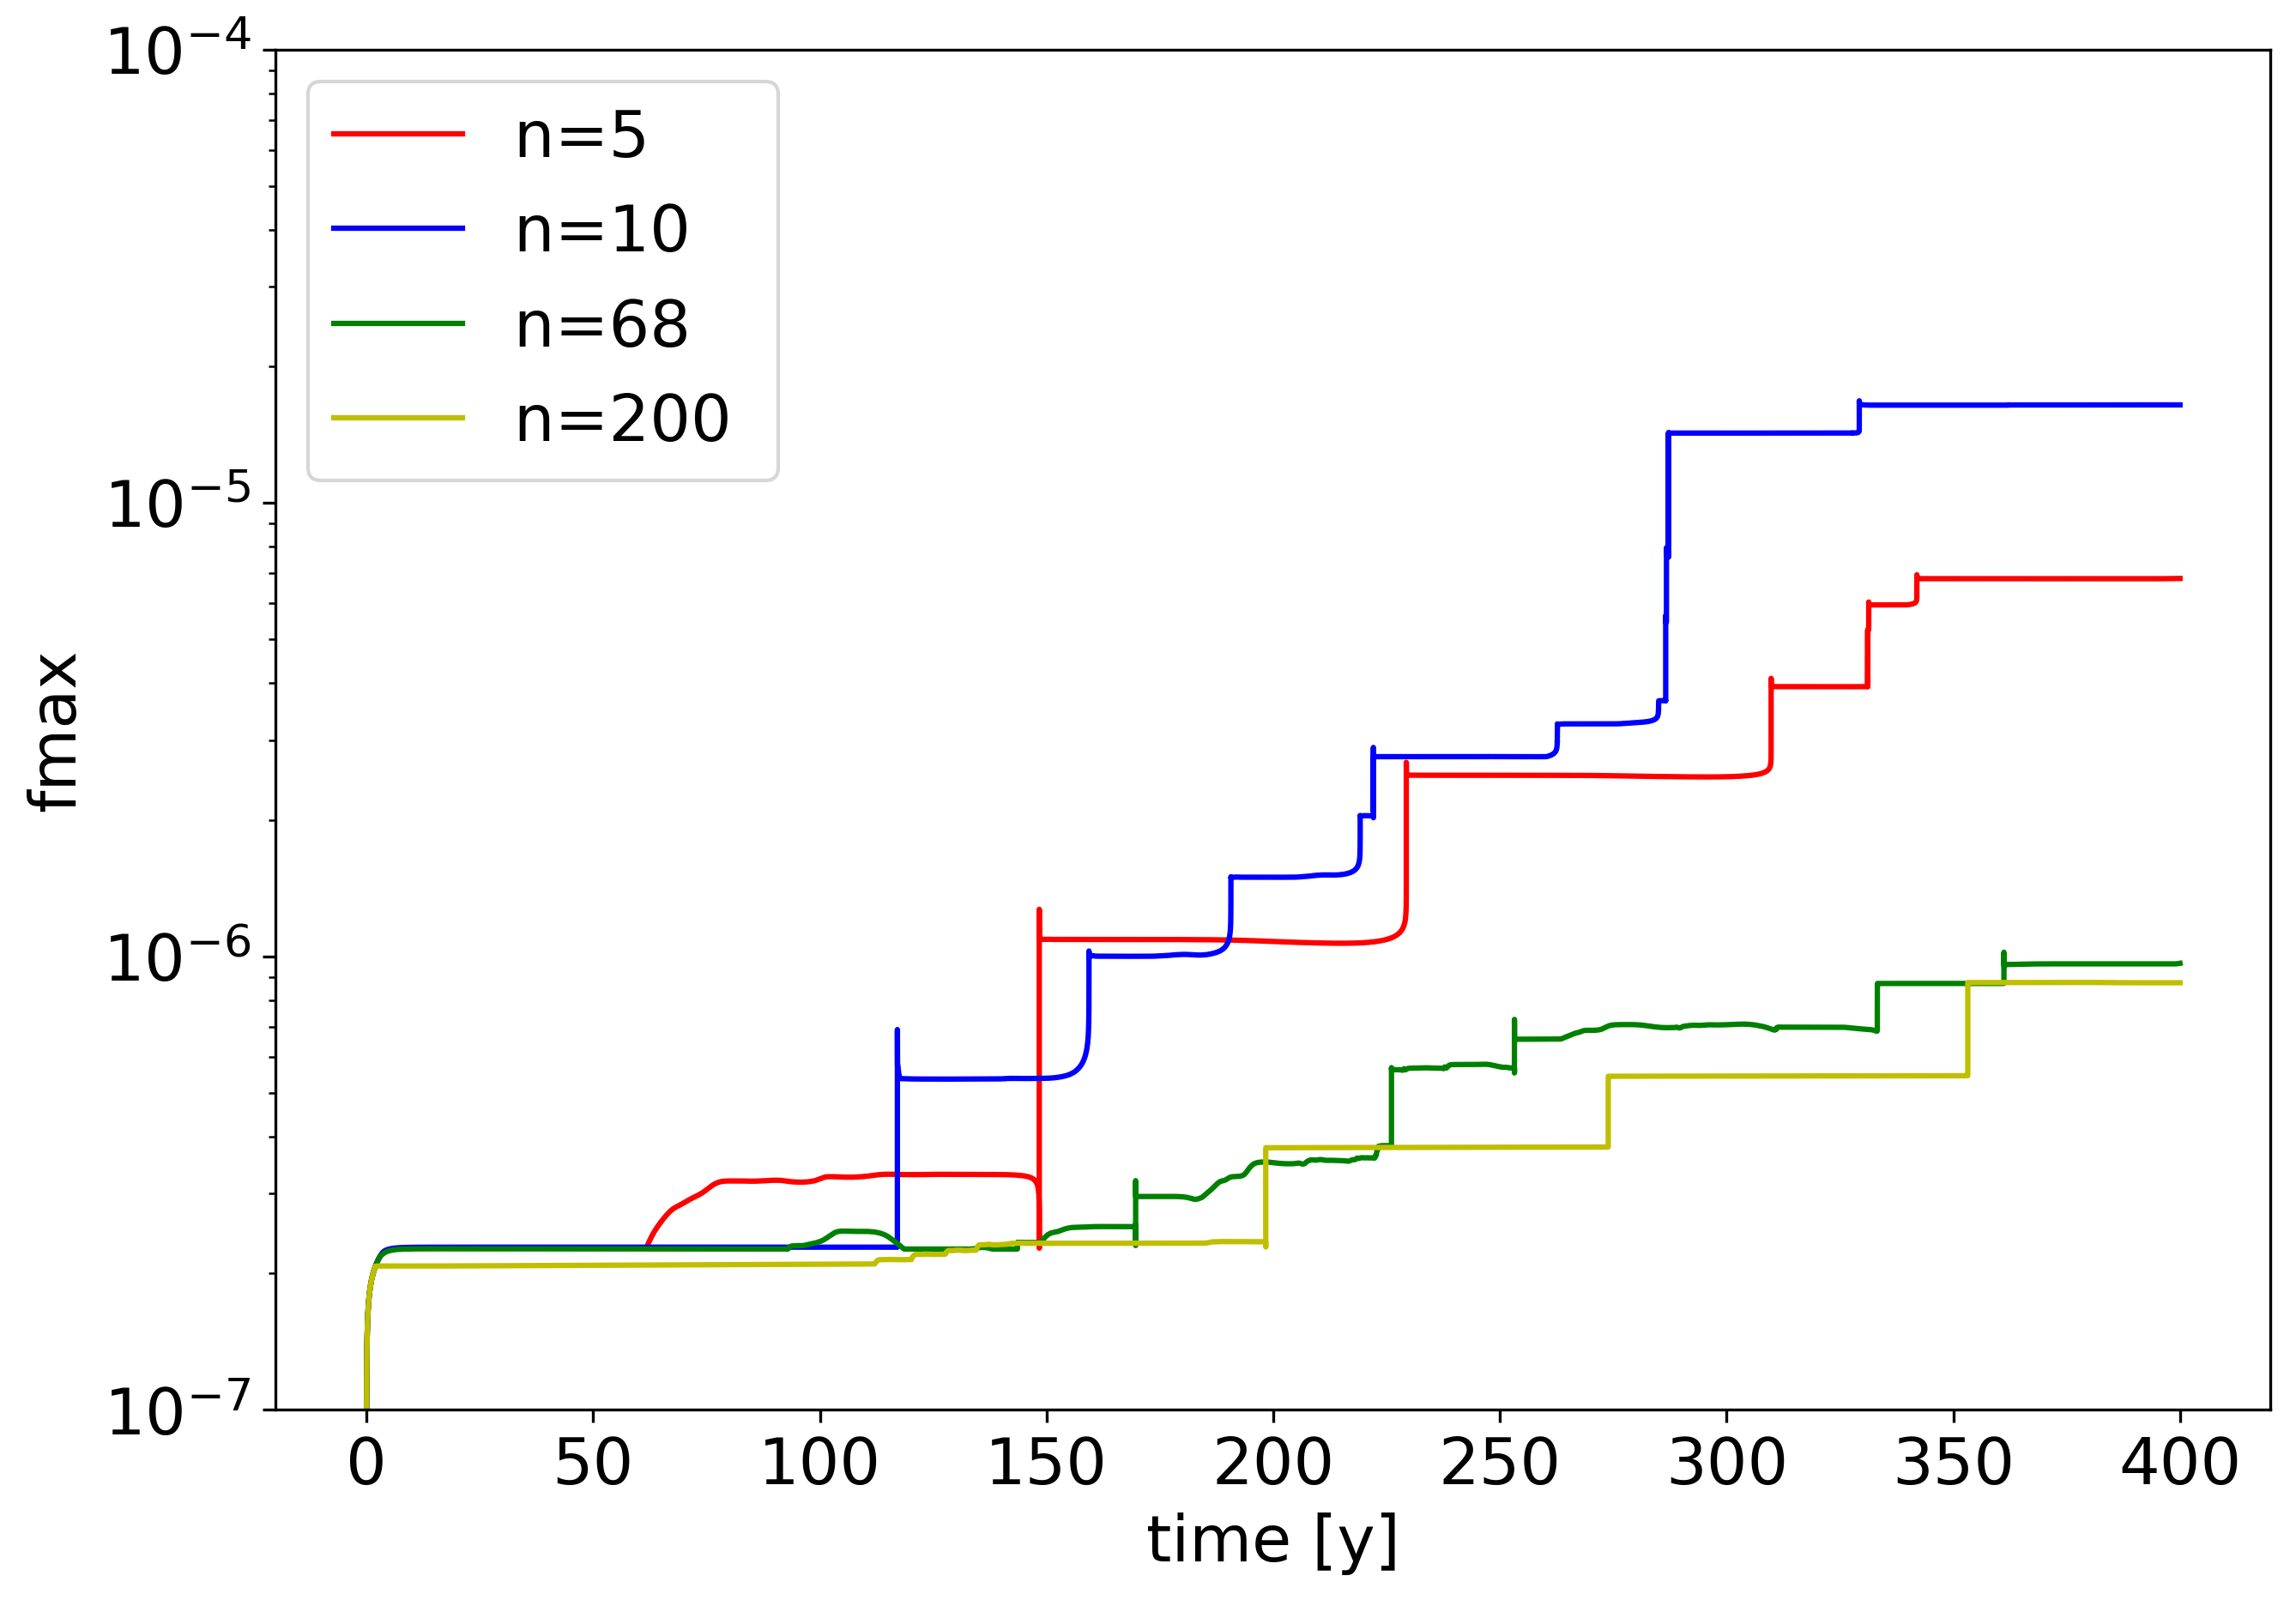
\includegraphics[width=1\textwidth]{images/TANDEMtimeEvolutionFExtendedODEDifferentSizes.png}
		\subcaption{Fixed tolerance at $t_r=10^{-8}$} 
		\label{fig:timeEvolution_2ndOrderODE_differentSizes}
	\end{subfigure}
	\label{fig:timeEvolution_2ndOrderODE}
	\caption{Evolution of the residual value of the friction law using the 2nd order ODE formulation over 400 years for varying relative tolerances in $V$ and mesh resolutions}
\end{figure}

Next, we investigate whether other parameters, such as the mesh resolution, affect the global error too. For a fixed relative tolerance for the slip of $10^{-8}$, the simulation has been executed for different numbers of fault elements and the evolution of the friction law in each case is shown in \autoref{fig:timeEvolution_2ndOrderODE_differentSizes}. Since each fault element contains three fault nodes, one has to multiply $n$ by three to obtain the total number of simulated fault nodes. In the beginning, all domain sizes have similar accuracy, but after some earthquakes, it seems that the residual in domains with higher resolution increases slower. \\

Overall, the evaluation of the friction law is a suitable estimate for the global error in the system. Over time, its value increases sharply at each earthquake, but overall linearly, which is due to a regular local truncation error. The main driver of the LTE is the tolerance for the slip rate $V$, which has been introduced to the system along with the second order ODE formulation. The upper bound for the LTE is proportional to the chosen tolerance. Even after 400 years, the residual of the friction law is acceptably low if the relative tolerance for the slip rate is set to $10^{-6}$ or below.


\section{Adaptivity of BDF methods}
\label{sec:Results_BDFOrder}
BDF methods exist for orders 1 to 6 and two error estimates have been introduced that can be used by the timestep controller. This section aims to compare and optimize these parameters with respect to the timestep size. The simulation has been run using the extended DAE formulation for 101 fault elements over 250 years, thus with one earthquake event.

\subsection{Quality of the error estimates}
Two error estimates have been introduced for the BDF methods in \autoref{sssec:errorEstimateBDFLagrange}. For the embedded method, at each time step a BDF scheme with higher order is applied to the current solution vector and the difference between both available solutions at the timestep yields the error estimate. The second method bases on the derivatives of Lagrangian polynomials and has the advantage to be much cheaper to evaluate since it does not require solving the system again. It has already been shown in \autoref{ssec:QualityErrorEstimate_0D} for the 1D example, that the first method gives a more accurate estimation of the local truncation error than the second method. Both methods tend to overestimate the error, which is undoubtedly a safe behavior, but restricts the choice of the next timestep. \\
Since here no exact solution is available for any physical quantity, the accuracy of the error estimate cannot be directly determined as previously. Instead, we assume that the actual error is inferior to the estimate and that the embedded method is more accurate than Lagrangian polynomials. We would then expect the timestep adapter to choose larger timesteps with the first method and finish the program earlier. This first section aims to see whether the more accurate embedded method allows for larger timesteps than the error estimate with Lagrangian polynomials and if so, whether the total number of timesteps can be reduced enough to justify the higher costs of the embedded method. \\
The first assumption is verified in \autoref{fig:BDFOrders_Lagrange_vs_Embedded_extended_DAE} for the extended DAE formulation. As expected, the embedded method is faster than Lagrangian polynomials, as features of the curve such as an increase or decrease of the timestep size happen increasingly earlier with 

\begin{figure}[H]
	\centering
	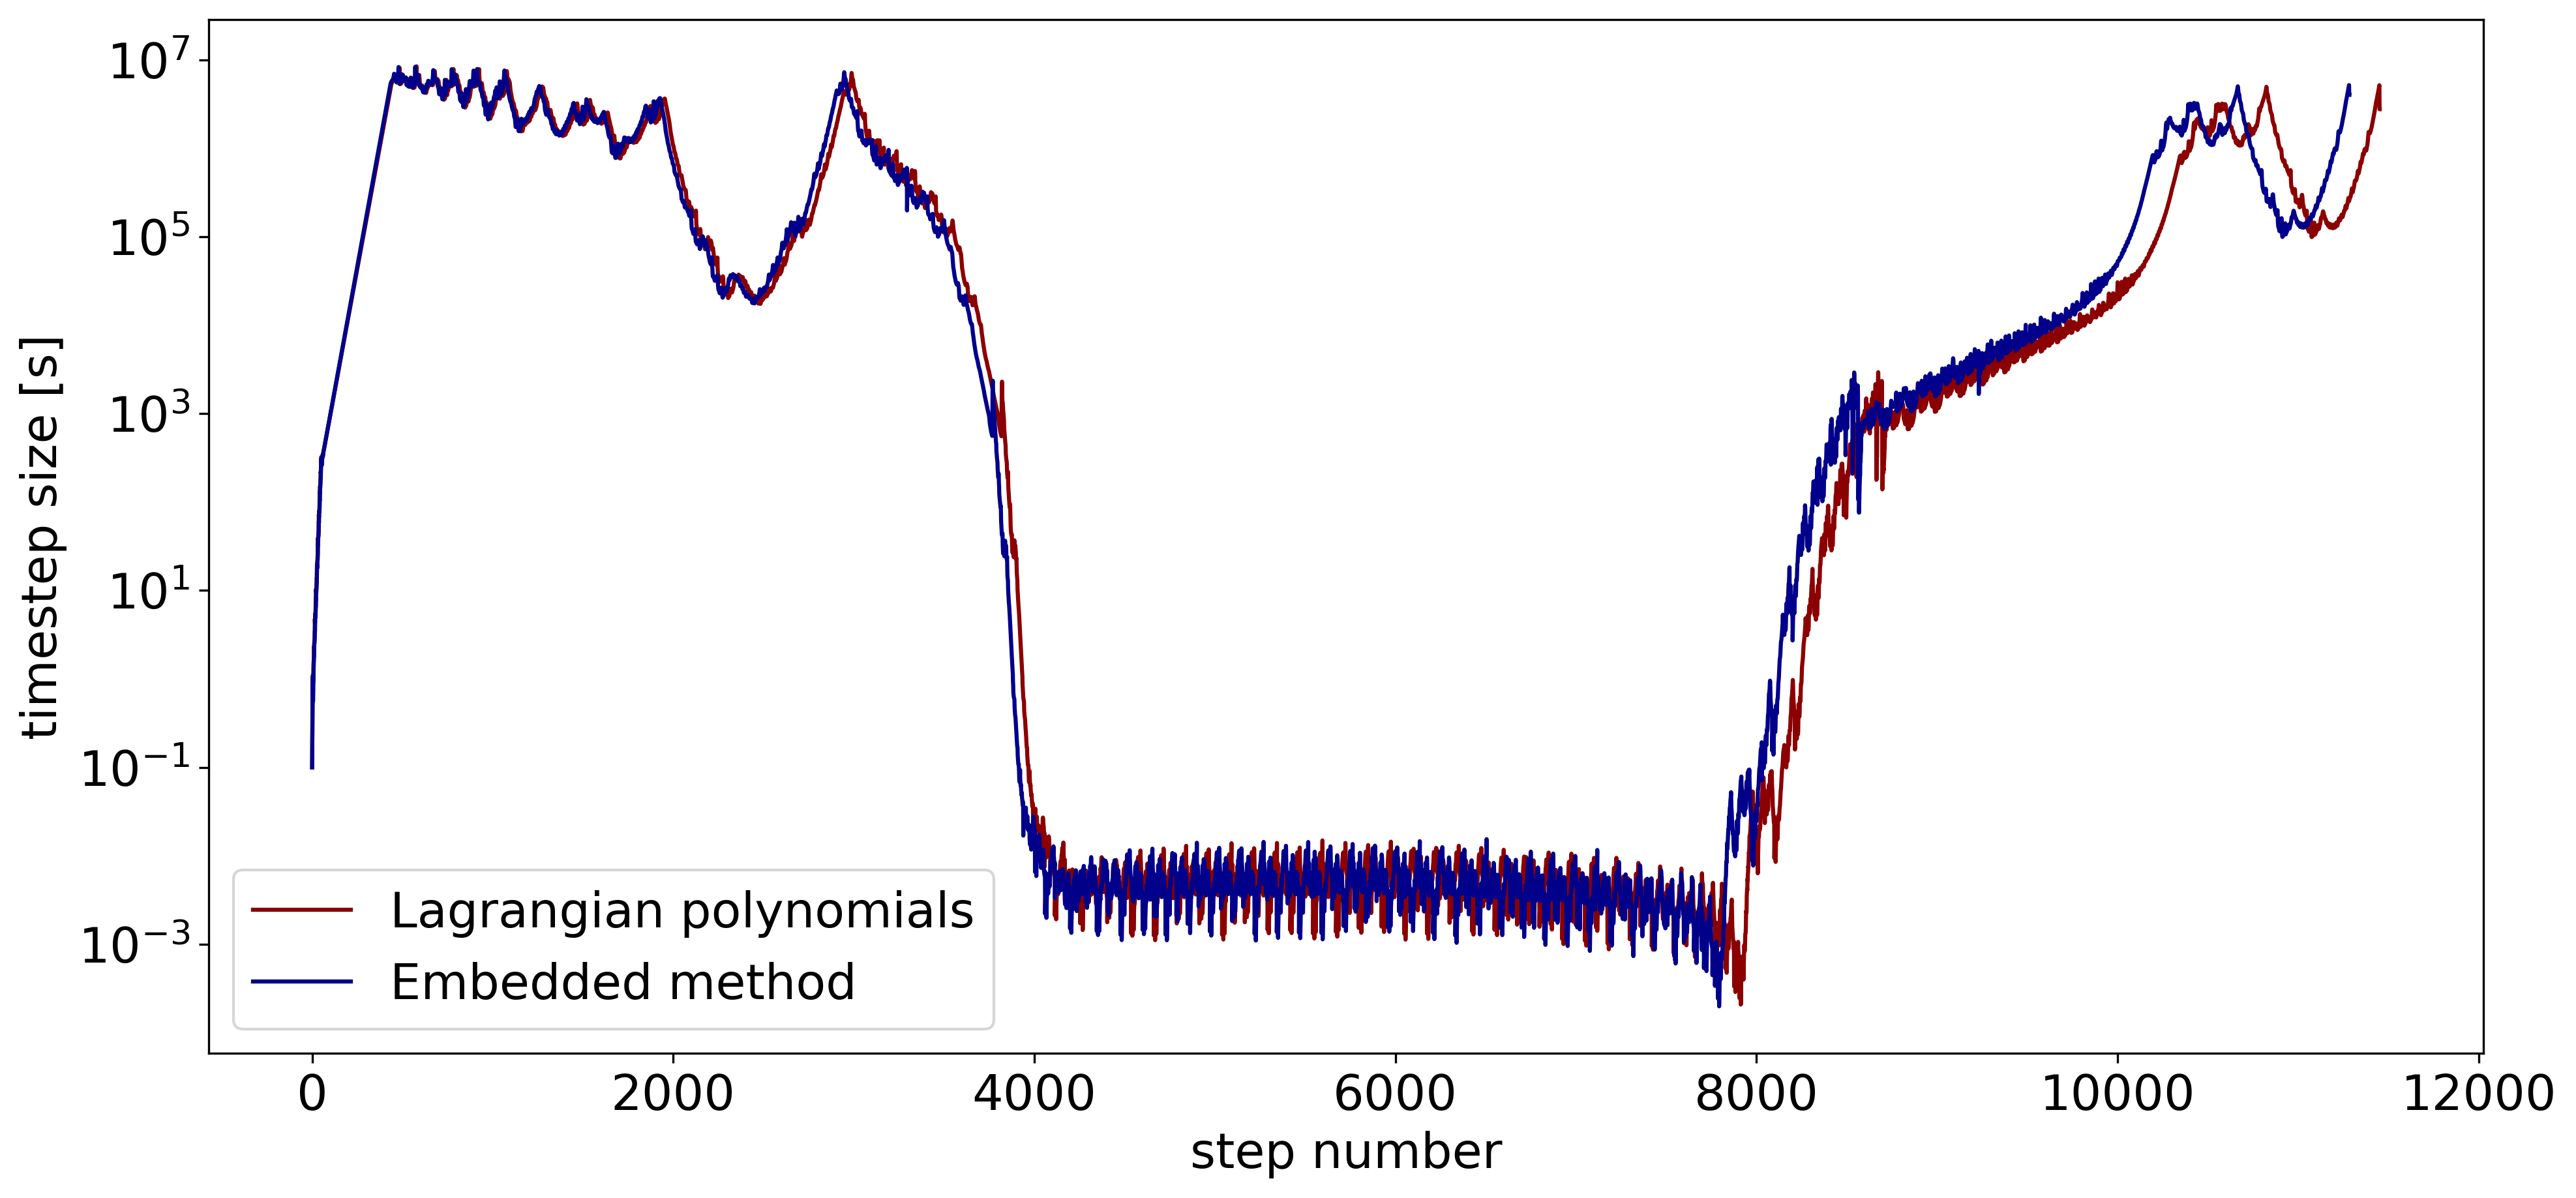
\includegraphics[width=0.8\textwidth]{images/TANDEMTimeAnalysisDifferentBDFOrdersEmbedded_vs_Lagrange_ExtendedDAE_Size101.png}
	\caption{Comparison of the chosen timestep sizes with the error estimates by Lagrangian polynomials and by an embedded method with a 5th order BDF method on a domain with 101 fault elements using the extended DAE formulation. }
	\label{fig:BDFOrders_Lagrange_vs_Embedded_extended_DAE}
\end{figure}

\noindent the embedded method. All in all, fewer timesteps are required to reach the end of the simulation. However, the allowed timesteps are only slightly larger and the difference cannot be noticed on the logarithmic scale. Nonetheless, it is positive to remark that the same small features such as intermediate peaks are observed with both methods, which indicates that both error estimates recognize the same inconsistencies in the solution. \\
Overall, the embedded method gives a more accurate error estimate than the Lagrangian polynomials and allows for larger timestep sizes. However, the gain is only very small, as on average 2\% fewer timesteps are required at the end of the simulation, and this does not justify the use of the embedded higher-order BDF method as an error estimate since it is twice as expensive. Actually, carefully choosing the order of the BDF method has a much higher potential to reduce the total number of iterations, as it will be discussed in the following section.

\subsection{Effect of the BDF order on the timestep size}
The simulation can be roughly split into four sections: the evolution of the aseismic slip, with an approximately constant stepsize of the order of $h=10^6$s, the evolution of the earthquake at $h=10^{-2}$s and the transition between both phases, where the stepsize progressively increases or decreases. In addition to that, there is the initialization phase, in which the stepsize starts at $h=0.1$s to quickly reach the stepsize of the aseismic slip. \\
The transition from the aseismic slip to the earthquake is a crucial section because the sudden increase of the slip rate requires rapidly scaling down the timestep size. The end of the earthquake is less critical, as the slip rate drops relatively slowly which gives more scope to the stepsize to adapt to it. Moreover the eventual too small stepsize at this point is not as problematic as a too high stepsize at the beginning of the earthquake. It is also interesting to look at the initialization phase, as there are no other constraints for a small stepsize but the limitations of the BDF scheme. In this section, we investigate the ability of BDF schemes of different orders to rapidly scale the timestep size up or down. \\
\autoref{fig:BDFOrders_extended_DAE_compare_initialization} shows the increase at the beginning of the simulation for the BDF methods of order 3-6 and \autoref{fig:BDFOrders_extended_DAE_compare_begin_first_EQ} shows the transition from the aseismic slip to the first earthquake. In the initialization phase, the slope is in general steeper if a higher-order method is used. One notable exception is the 6th order BDF scheme, which has a lower slope than expected. Unlike the other schemes, it does not increase smoothly but has regular steps, which indicates that the 6th order scheme is not as stable as the others. It seems that it first tries to increase the timestep size by a large factor, but has to correct it down after a few steps again because the error tolerance is not respected. Overall, the increase is perfectly exponential for the schemes 3-5, and the factor by which the timestep size increases at each step is driven by the order of the method. Interestingly enough, in the very first timesteps,  the timestep size of the 2nd order scheme jumps by two orders of magnitude whereas the 5th and 6th order do not benefit at all from such a strong initial increase. 

\begin{figure}[H]
	\centering
	\begin{subfigure}[b]{0.45\textwidth}
		\centering
		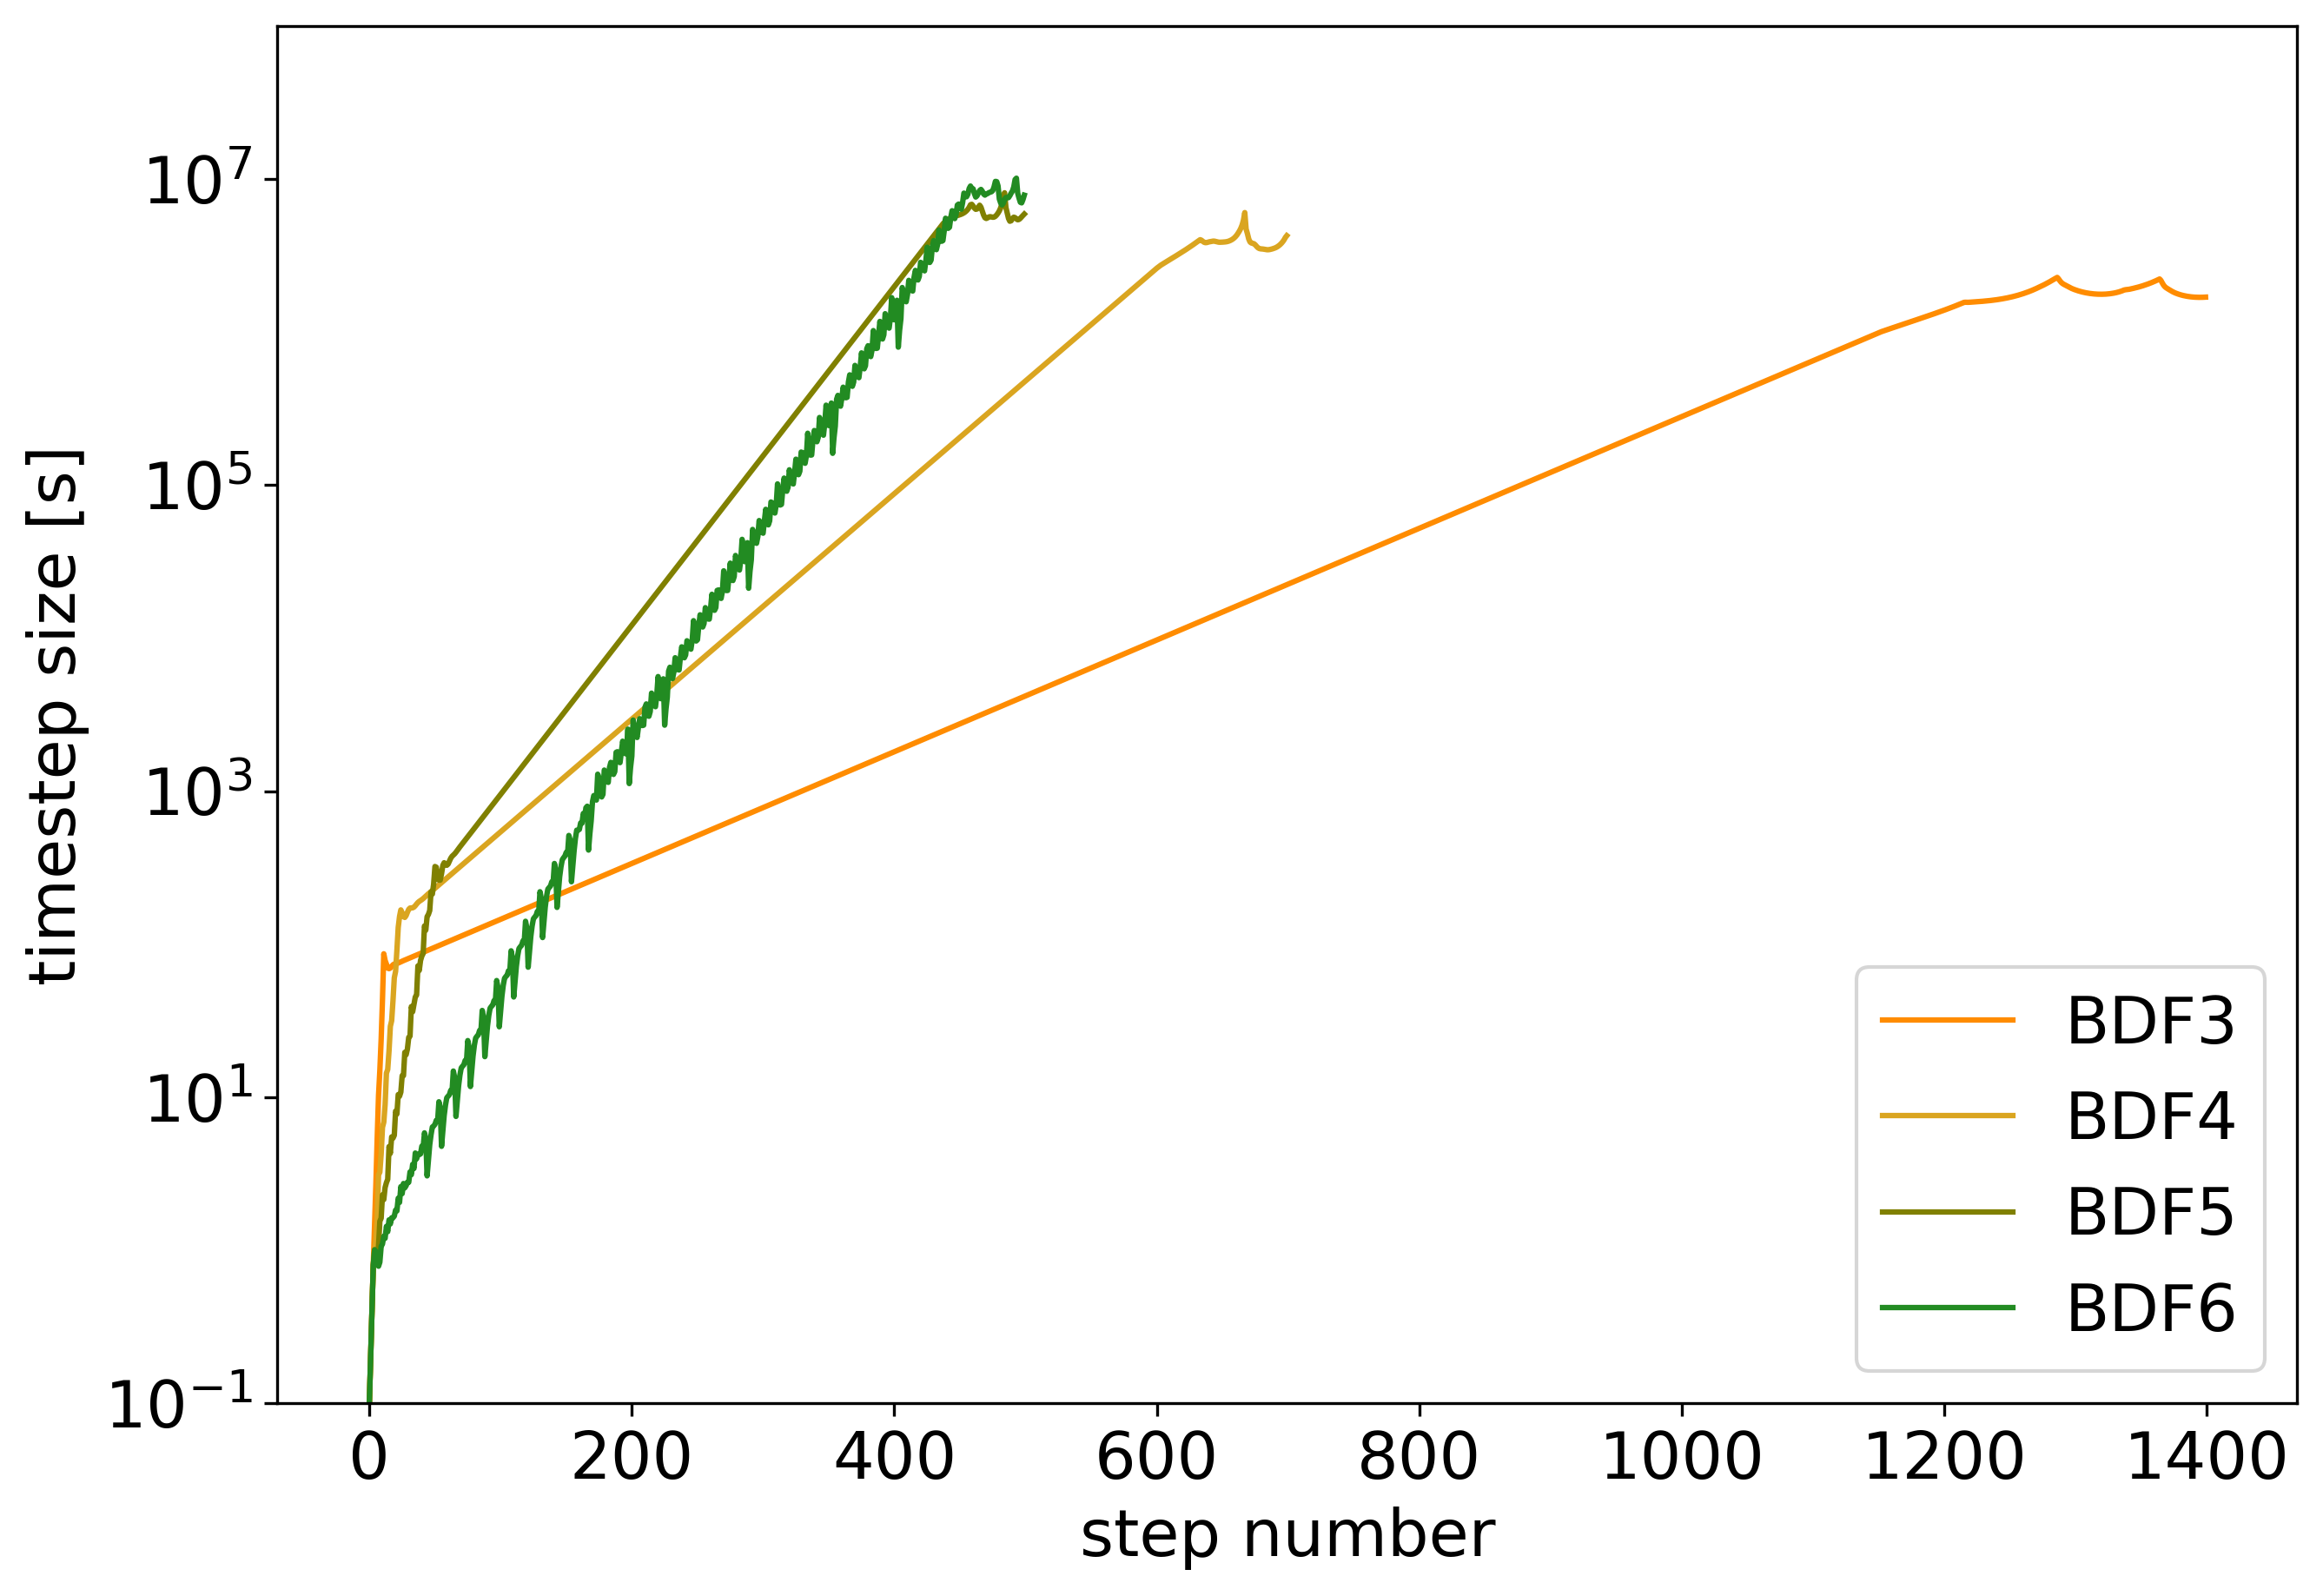
\includegraphics[width=1\textwidth]{images/TANDEMTimeAnalysisDifferentBDFOrdersLagrange_ExtendedDAE_Size101_Init.png}
		\subcaption{At the beginning of the simulation \\ \ } 
		\label{fig:BDFOrders_extended_DAE_compare_initialization}
	\end{subfigure}
	\begin{subfigure}[b]{0.45\textwidth}
		\centering
		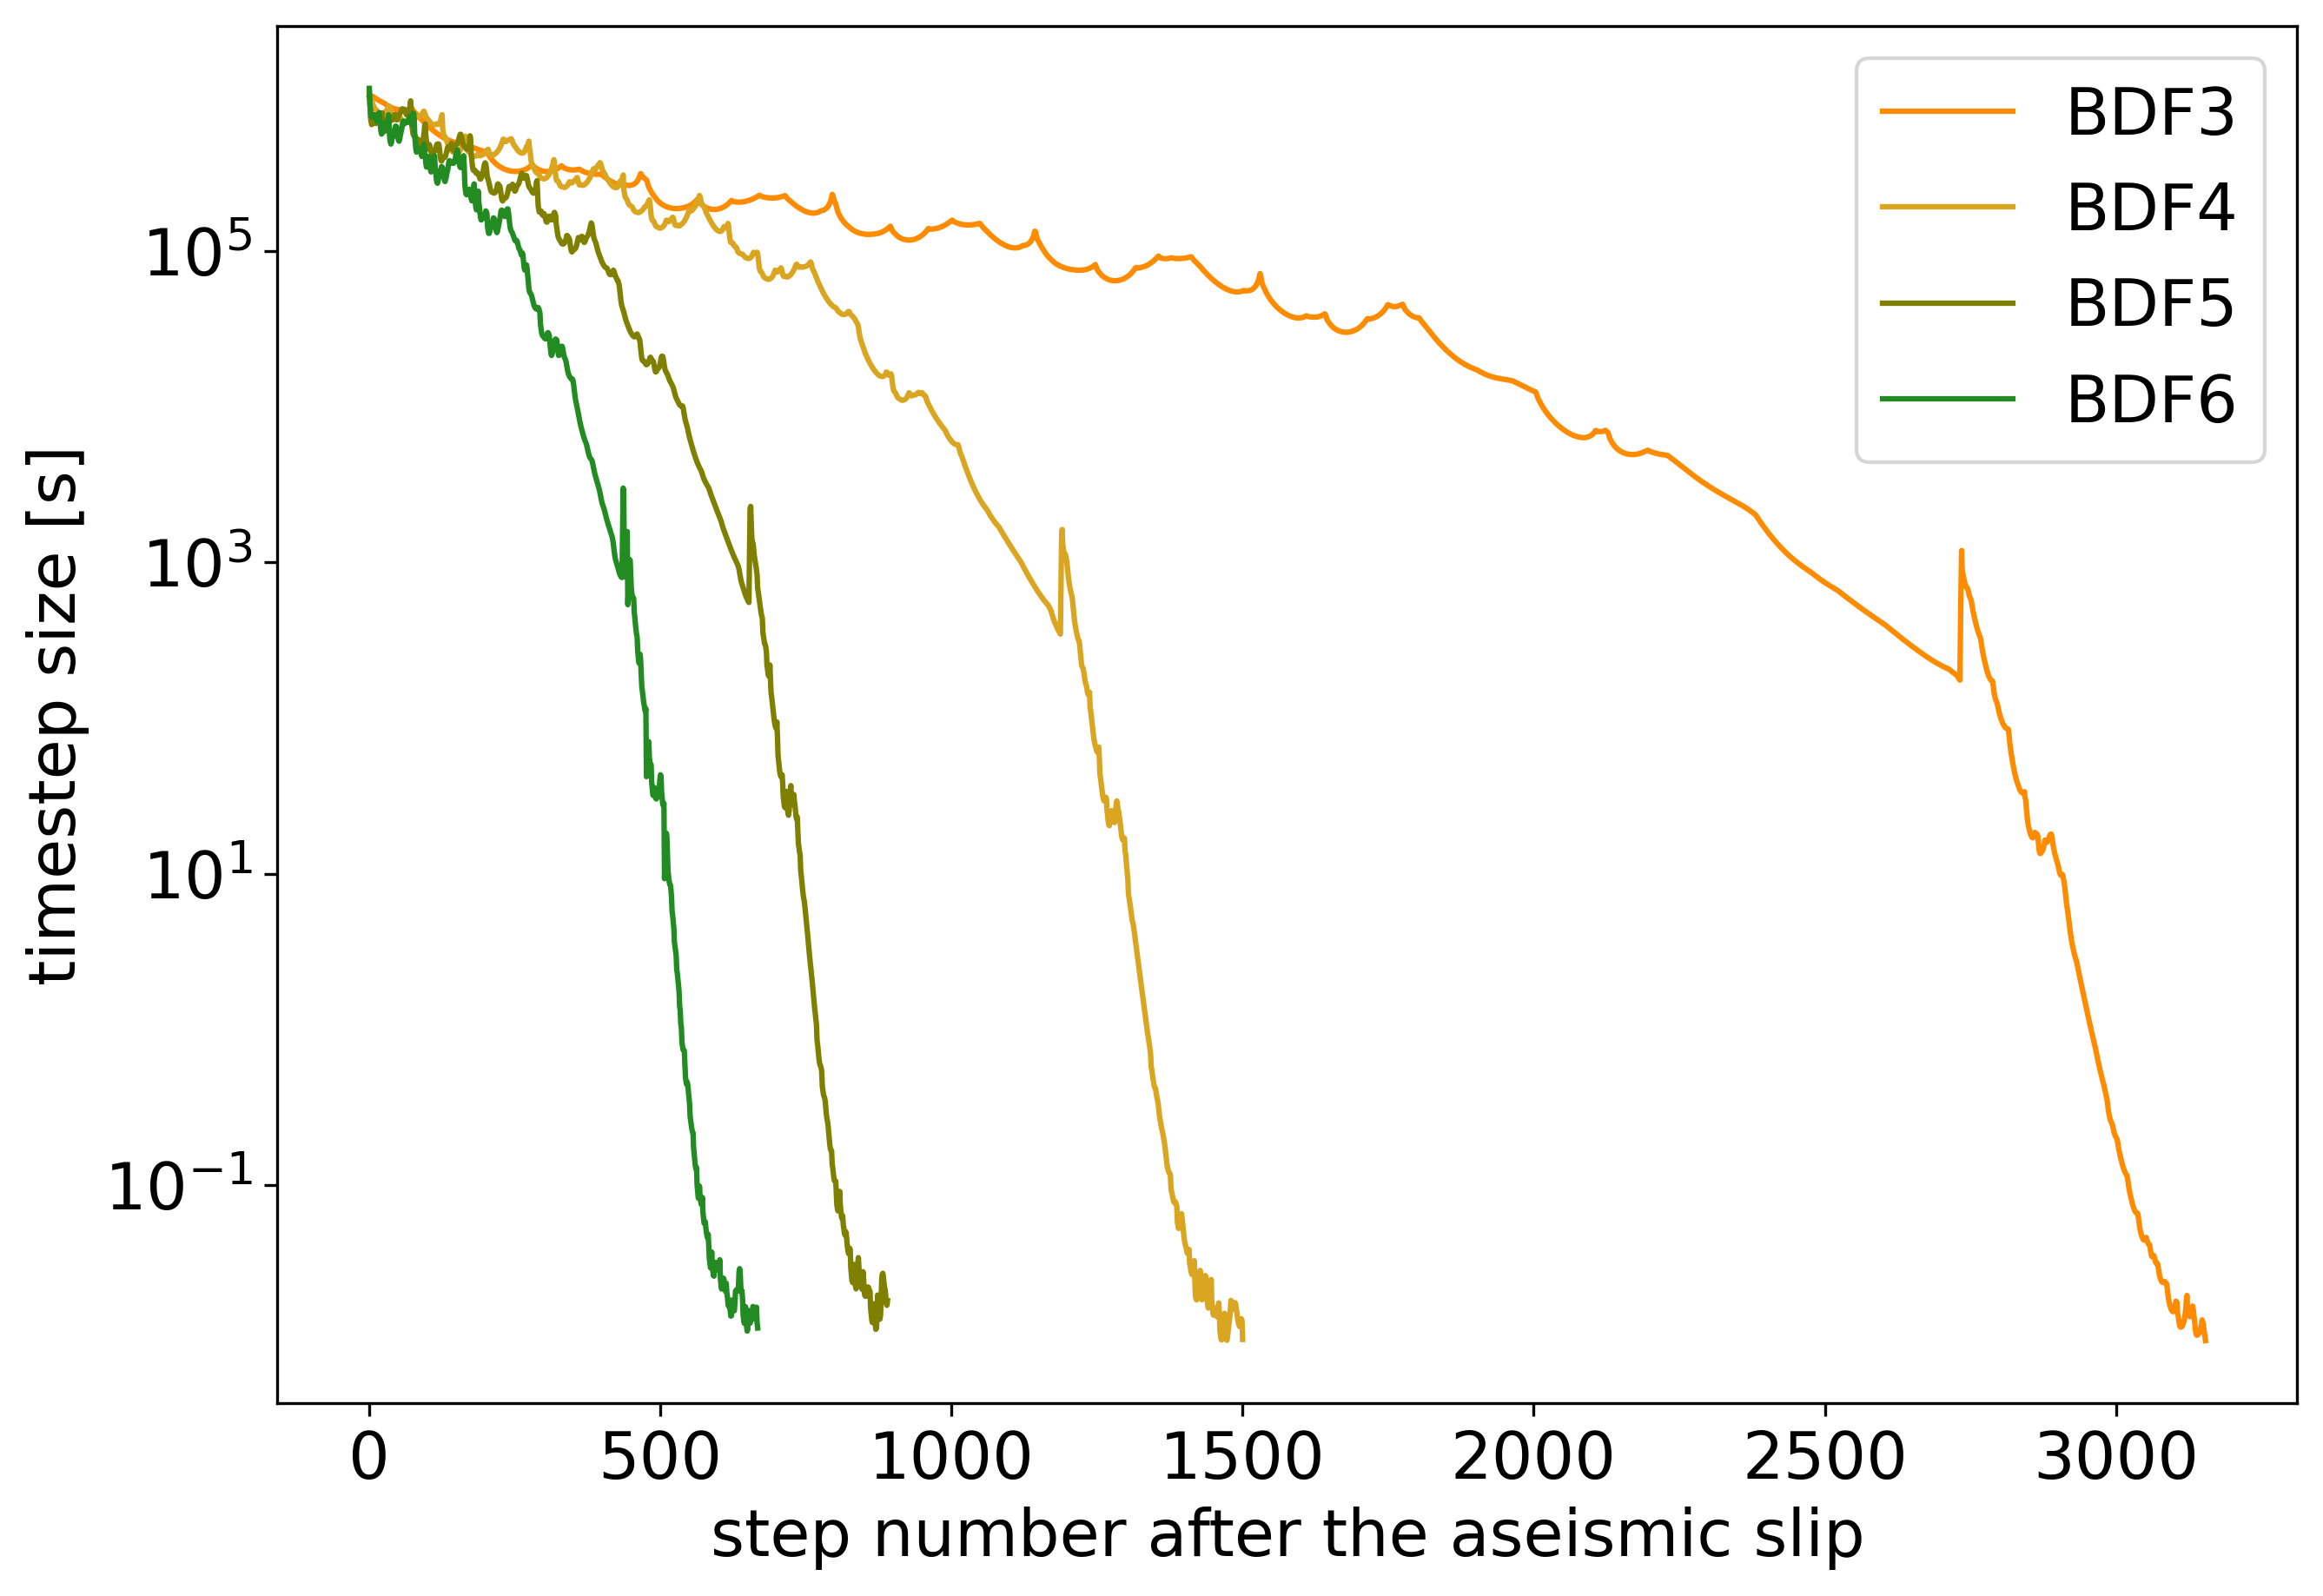
\includegraphics[width=1\textwidth]{images/TANDEMTimeAnalysisDifferentBDFOrdersLagrange_ExtendedDAE_Size101_Begin1stEQ.png}
		\subcaption{At the transistion from the aseismic to the earthquake phase}
		\label{fig:BDFOrders_extended_DAE_compare_begin_first_EQ}
	\end{subfigure}
	\caption{Evolution of the time step size for BDF schemes with different order at key points in the simulation on a domain with 101 fault elements using the extended DAE formulation.}
\end{figure}

At the transition from the aseismic phase to the earthquake phase, the timestep size decreases exponentially with the same pattern: a higher order scheme allows a stronger reduction of the timestep size from one step to the next. Now, the 6th order scheme is perfectly stable and has the steepest slope among all BDF methods. \\

Higher order BDF methods allow in general for larger timestep sizes and are to be preferred over lower order methods. Since the costs of all BDF schemes are similar (they converge similarly fast and each Newton step always requires solving one linear system), there is no strong reason to prefer a low order scheme. Because of the stability issues with the 6th order scheme when the timestep size increases, the best performance can be expected from the 5th order scheme. There are a few cases where lower order methods perform better, such as at the very beginning of the simulation. \\

To take advantage of these peculiarities, and also to use the 6th order method if it is currently stable, the order of the BDF scheme can be adapted at each timestep as described in \autoref{sssec:adaptiveBDFOrder}. In this case, each step also calculates by how much the timestep size would change if one order higher or lower was used, and if a larger timestep can be reached, the order is changed accordingly for the next timestep. This has been implemented and the performance of the order-adaptive BDF scheme is shown in \autoref{fig:BDFOrders_extended_DAE_compare_adaptiveBDF}. It successfully uses the scheme with the largest allowable timestep size and finishes the simulation faster than any other methods, without any significant additional costs. 


\begin{figure}[H]
	\centering
	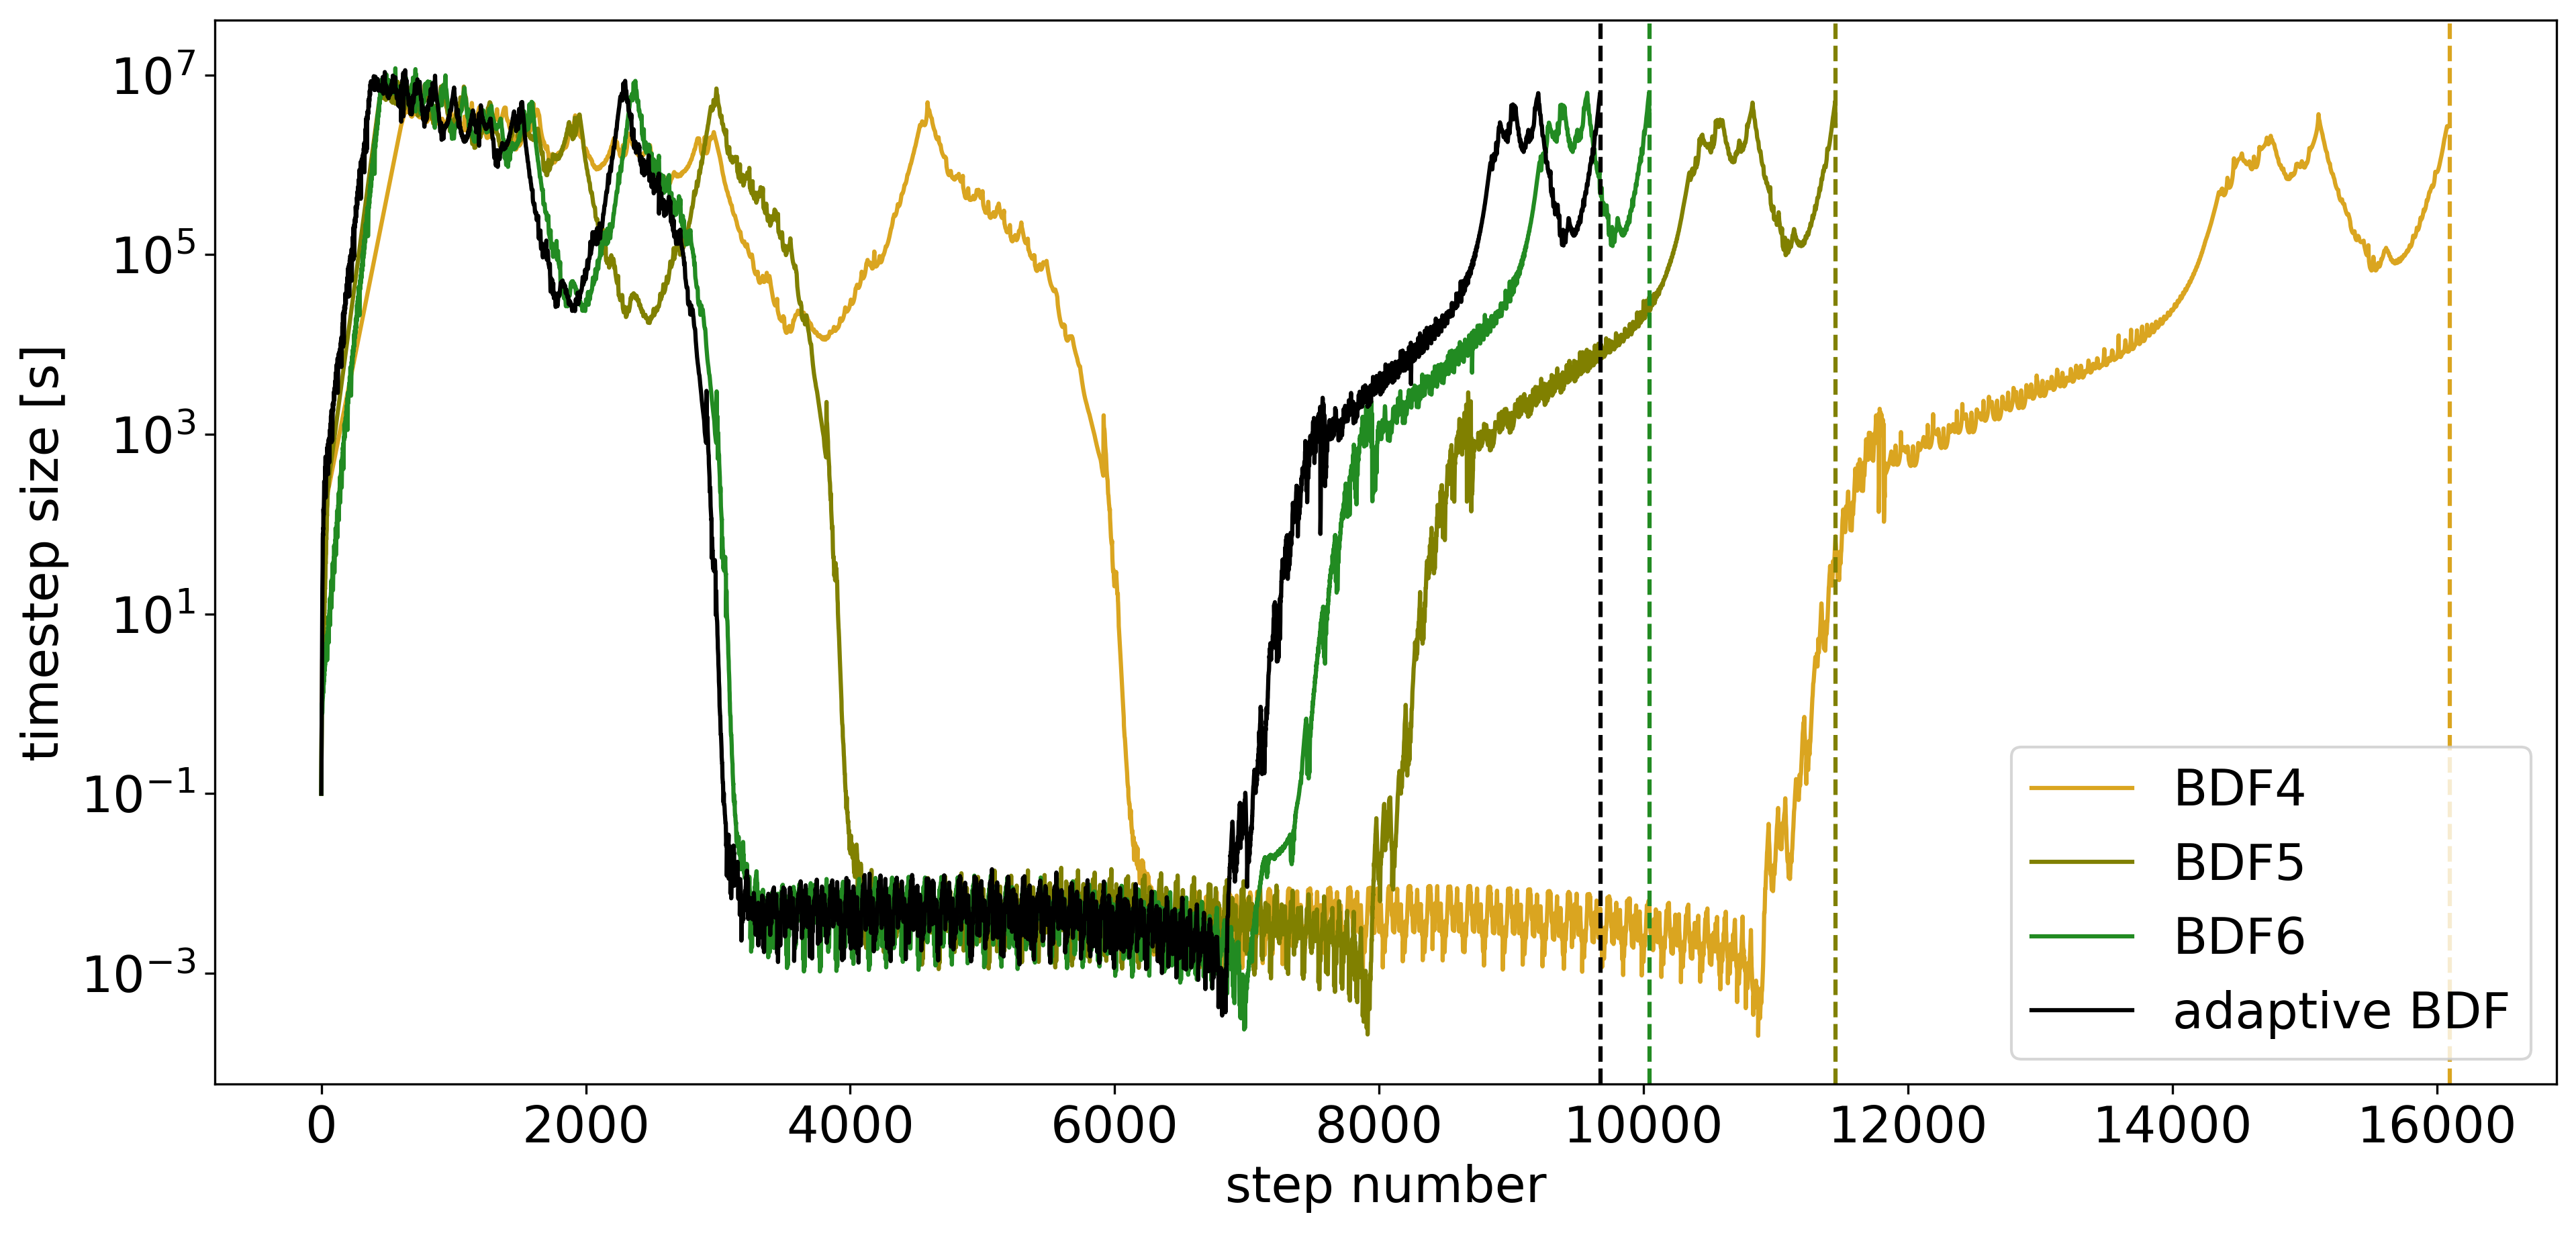
\includegraphics[width=0.8\textwidth]{images/TANDEMTimeAnalysisDifferentBDFOrders_Lagrange_ExtendedDAE_Size101_FULLTIME.png}
	\caption{Evolution of the time step size for the adaptive-order BDF method and for a selection of different fixed order methods on a domain with 101 fault elements using the extended DAE formulation.}
	\label{fig:BDFOrders_extended_DAE_compare_adaptiveBDF}
\end{figure}


\section{Scalability}
\label{sec:Results_Scalability}
This section aims to investigate how the time integration scales with the mesh resolution. To ensure comparability between the results, we set the tolerances such that the period between earthquakes and the slip increase are solved with similar accuracy. From the analysis in \autoref{sec:Results_AccuracyTimeIntegration}, we choose respectively $t_a^S=10^{-8}$ and $t_a^S=10^{-5}$ for the aseismic and earthquake phases for the first order formulations, and $t_r^V=10^{-8}$ and $t_r^V=10^{-7}$ for the second order ODE formulation. All simulations have been run on domains with 52, 101, 200 and 400 fault elements for a simulated time of 250 years. The results for the smallest domain size are not as revealing as the others because many false earthquakes are detected within the simulated time but none managed to increase significantly the slip at the open surface (see the discussion in \autoref{sec:2DSEAS__EvolutionOfQuantities}).

\subsection{Iterative schemes}
\label{ssec_Results_Scalability_IterativeSchemes}
Whereas the computational effort of a timestep with an explicit method is quite foreseeable, this is not true for implicit methods. Each step requires performing a Newton iteration, and within each Newton step, a linear system of equation is solved using the GMRES iterative solver with a SOR preconditioner. The problem size might affect the convergence speed of each of these iterative schemes and thus the overall performance of the simulation. All formulations can be solved implicitly, and the results are gathered in \autoref{fig:implicit_methods_scalabilty_iterations}. 

\begin{figure}[H]
	\centering
	\begin{subfigure}[b]{0.32\textwidth}
		\centering
		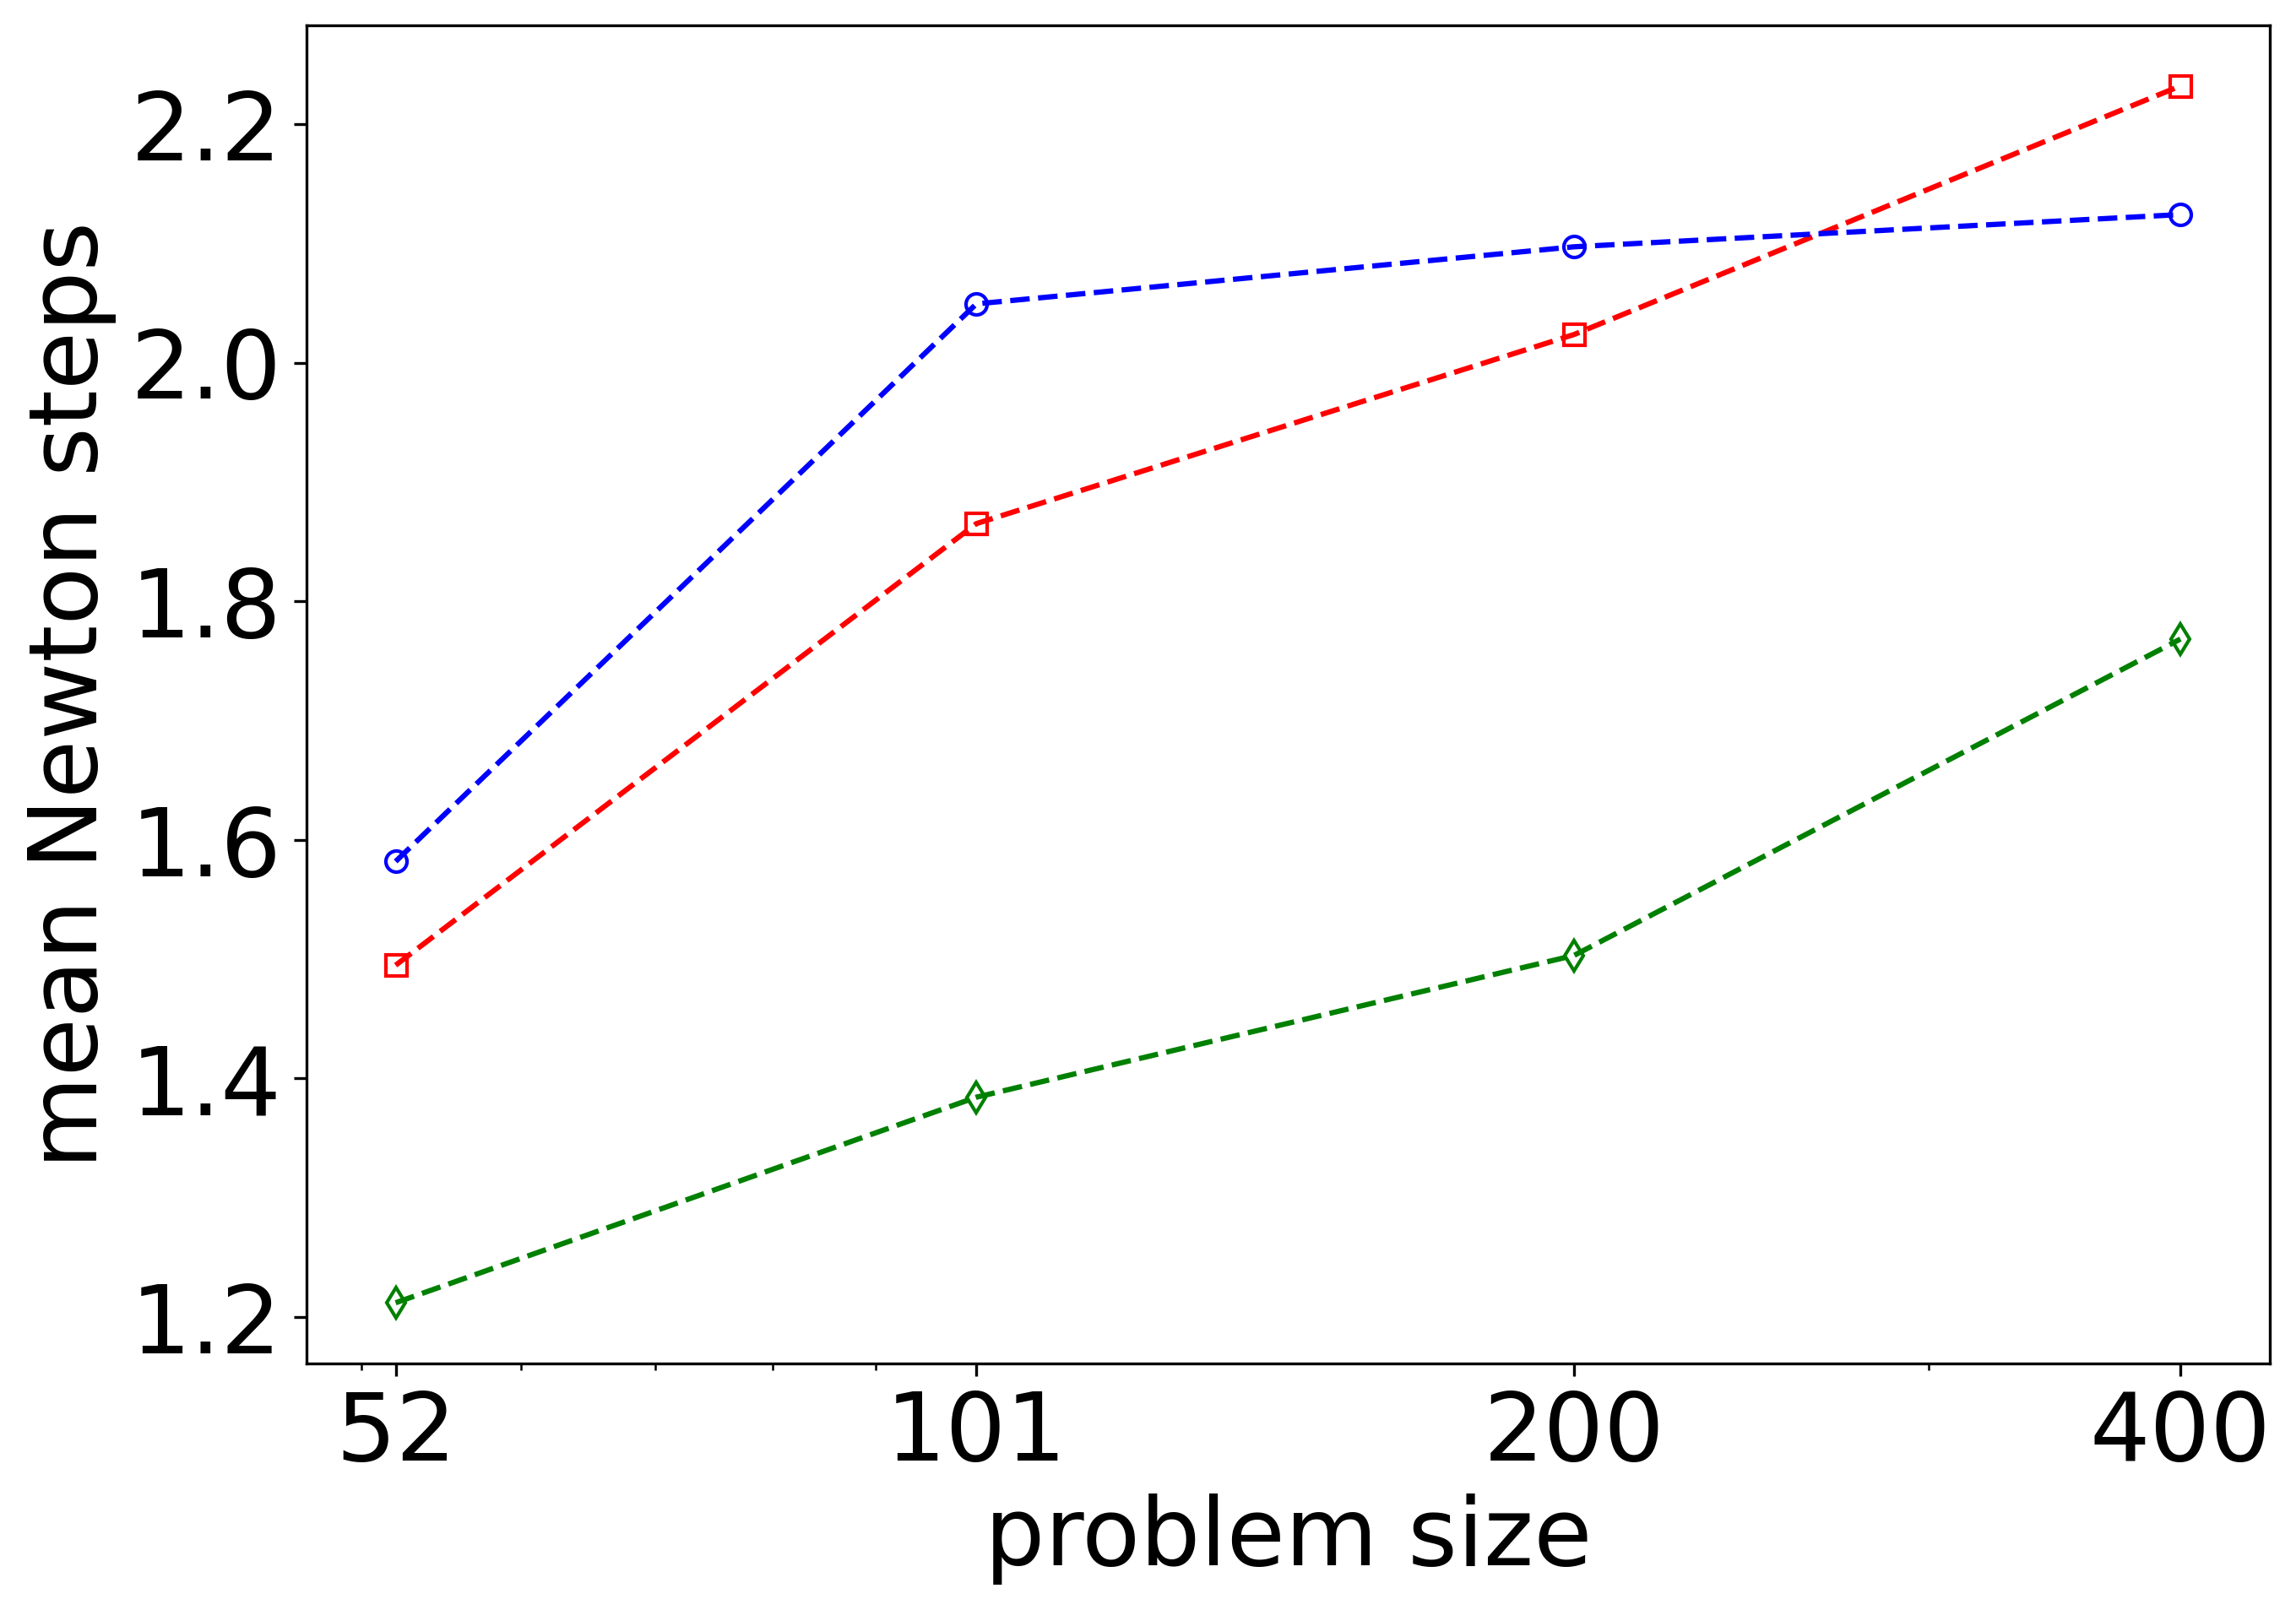
\includegraphics[width=0.97\textwidth]{images/TANDEM_averageNumberNewtonSteps.png}
		\subcaption{Average number of Newton steps per timestep \\ \ } 
	\end{subfigure} 
	\begin{subfigure}[b]{0.32\textwidth}
		\centering
		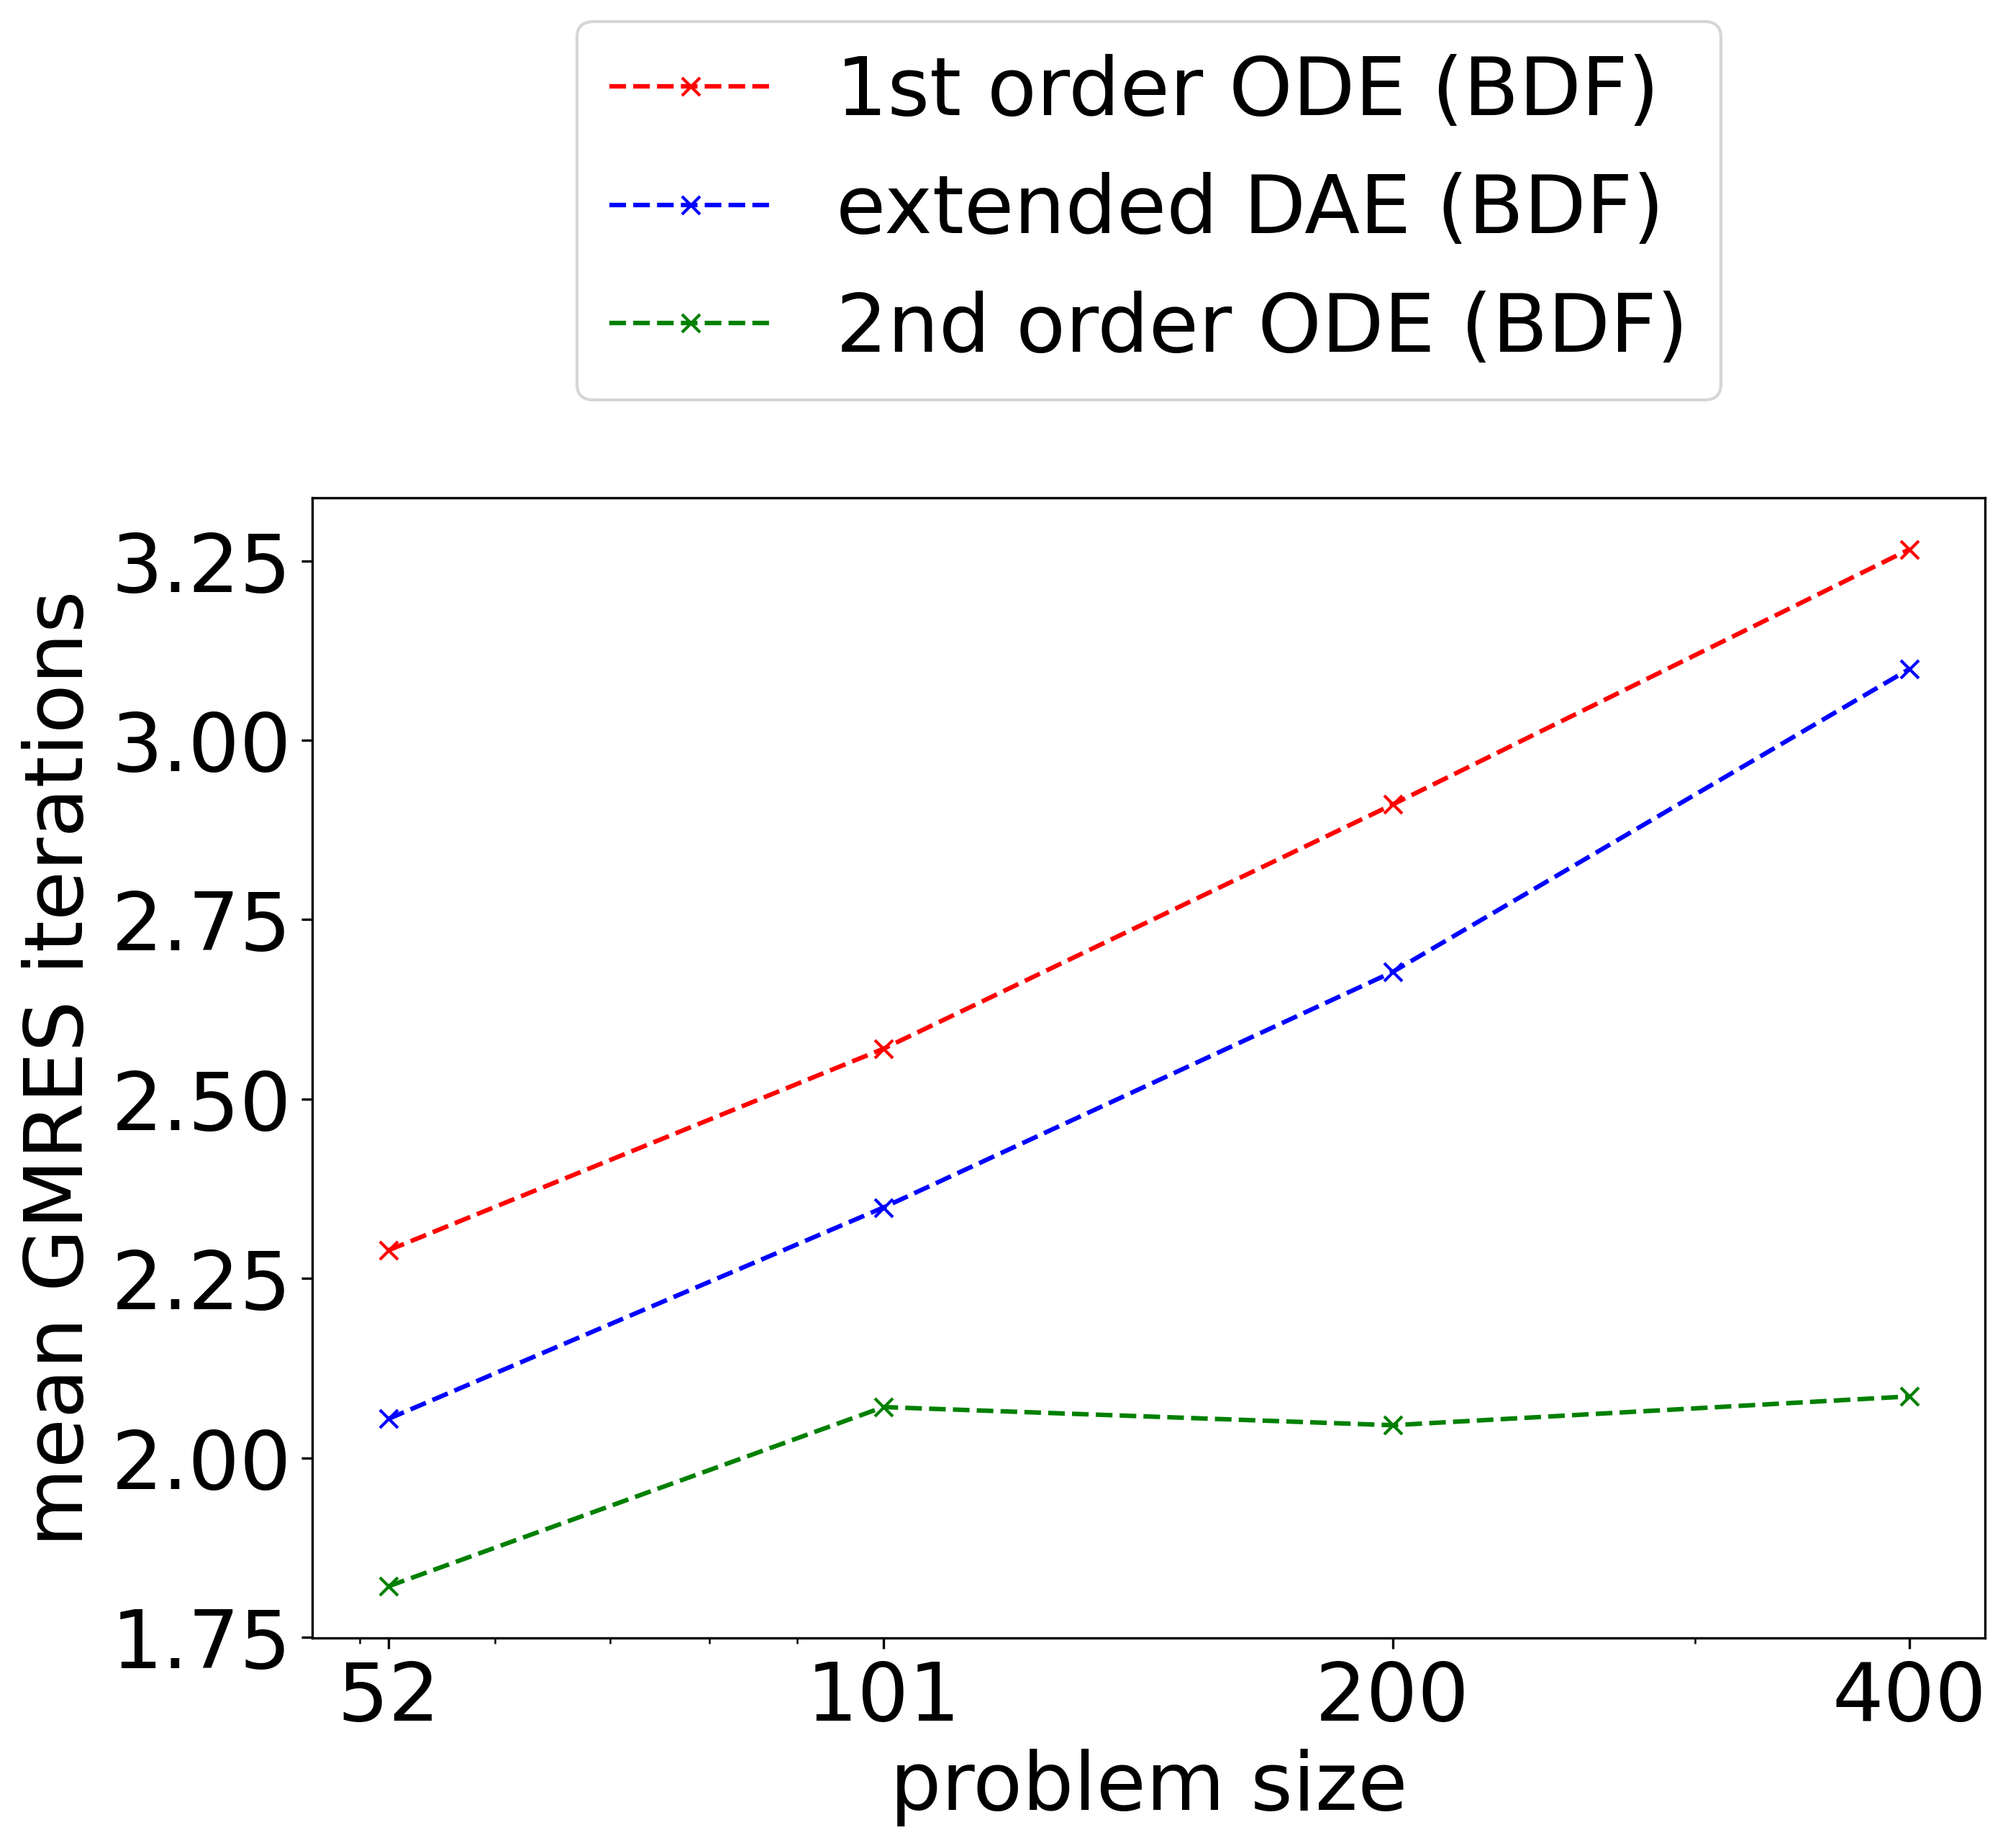
\includegraphics[width=1\textwidth]{images/TANDEM_averageNumberKSPIteration.png}
		\subcaption{Average number of GMRES iterations of the per Newton step} 
	\end{subfigure}
	\begin{subfigure}[b]{0.32\textwidth}
		\centering
		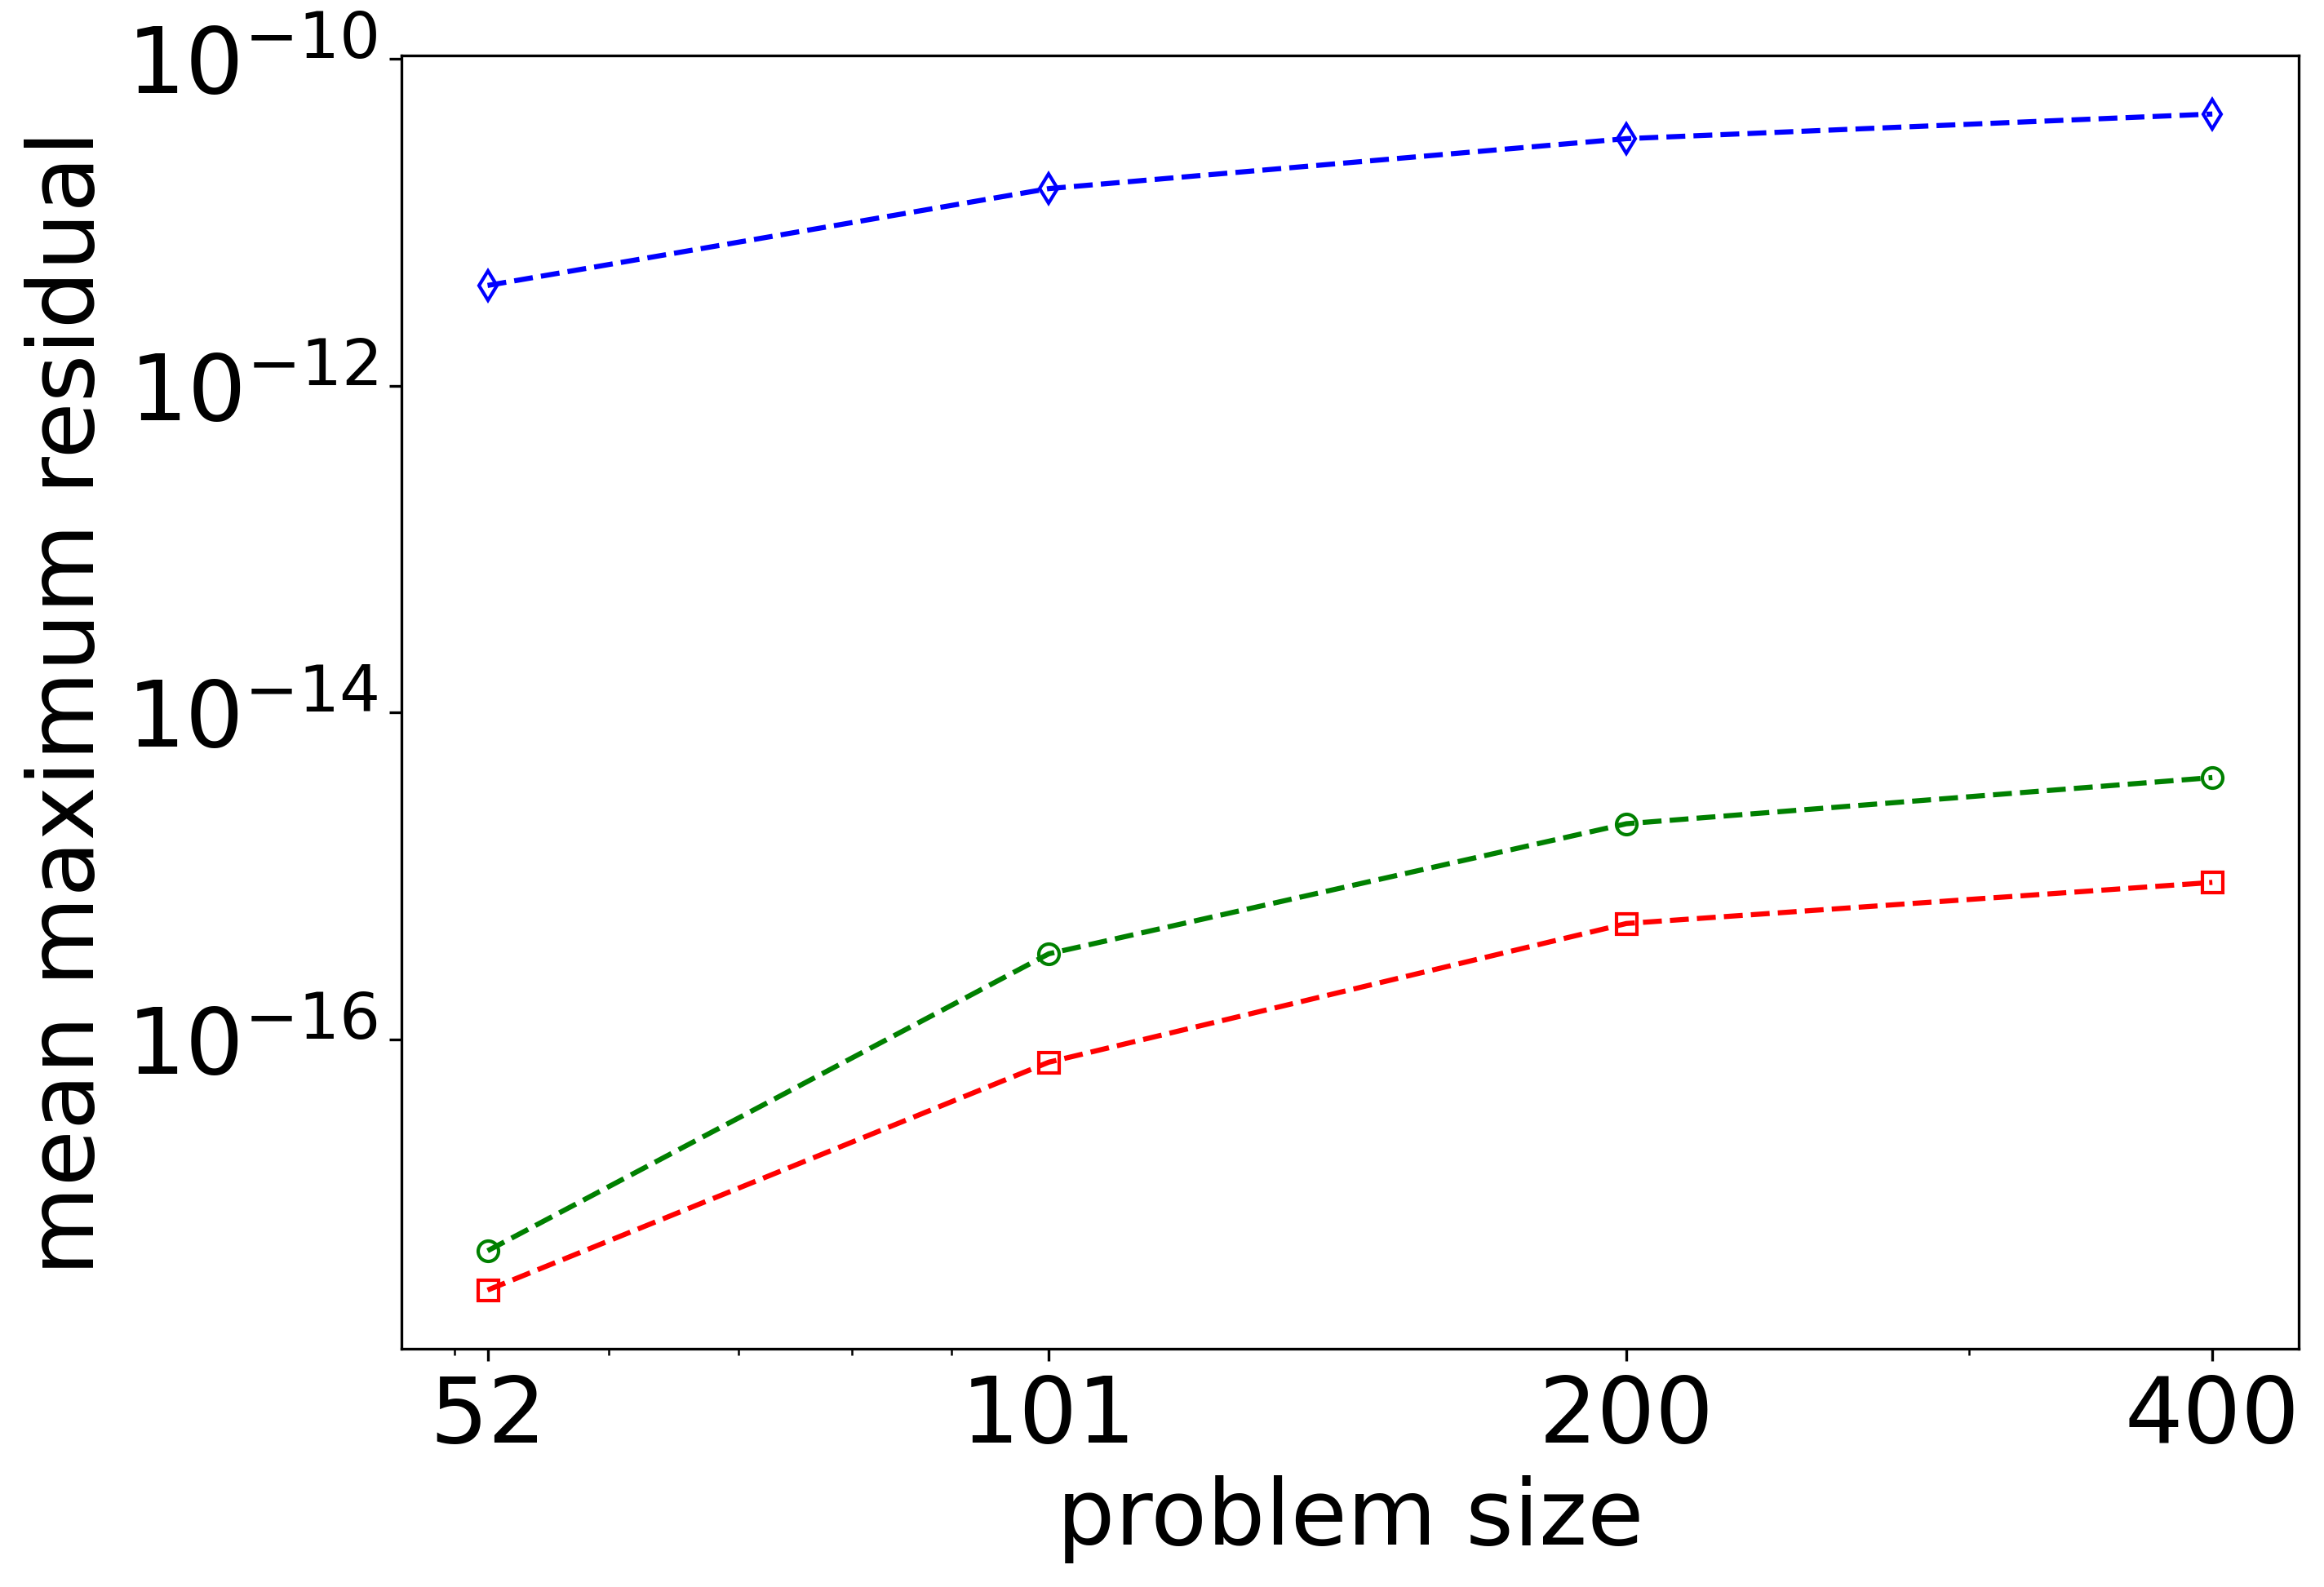
\includegraphics[width=1\textwidth]{images/TANDEM_maximumResidualNorm.png}
		\subcaption{Geometric mean of the final maximum norm of the residual} 
	\end{subfigure}
	\caption{Indicators of the Newton iteration for all formulations with an implicit time integration on different problem sizes. Note that each timestep includes one additional RHS evaluation before the Newton iteration.}
	\label{fig:implicit_methods_scalabilty_iterations}
\end{figure}

In both iterative schemes, the 2nd order ODE requires fewer steps to converge than both 1st order formulations. The more critical is the Newton iteration, as each Newton step requires performing a GMRES iteration and evaluating the RHS. Especially for the 1st order schemes, the latter involves solving the DG problem, which is the most expensive operations. Considering this, the extended DAE formulation scales much better with the problem size as it seems to remain at 2.1 iterations per timestep. For the two ODE formulations, it appears that the nonlinear Newton solver faces an increasing difficulty to match the required tolerance of $10^{-12}$. This can be also observed in subfigure (c), where the final residual norm considerably overshoots the tolerance value for small domains, but not for larger ones. Overall, the iteration number remains small, with up to 3 RHS evaluations until convergence. This is a clear advantage over explicit schemes, which always need to evaluate the RHS 6 times per timestep due to the formulation of the Runge-Kutta scheme. For the GMRES iteration, the two 1st order formulations require increasingly more steps to converge. However, the iteration number seems to depend logarithmically on the problem size and combined with the quadratic complexity of the GMRES scheme, it still scales better than the cubic complexity of the naive LU decomposition. 


\subsection{Timestep sizes}
\label{ssec:Results_scalability_timestepSizes}
An essential metric to compare the formulations is the evolution of the timestep size over the simulation. It has a direct impact on the length of the simulation: the larger the timestep size, the fewer timesteps are required and the faster the simulation reaches its end. The first five graphs in \autoref{fig:scalabilty_timeStepSizes} show the evolution of the timestep size for each possible combination of formulation and numerical integrator (BDF or RK), and the last graph depicts the total number of required timesteps.

\begin{figure}[H]
	\centering
	\begin{subfigure}[b]{0.32\textwidth}
		\centering
		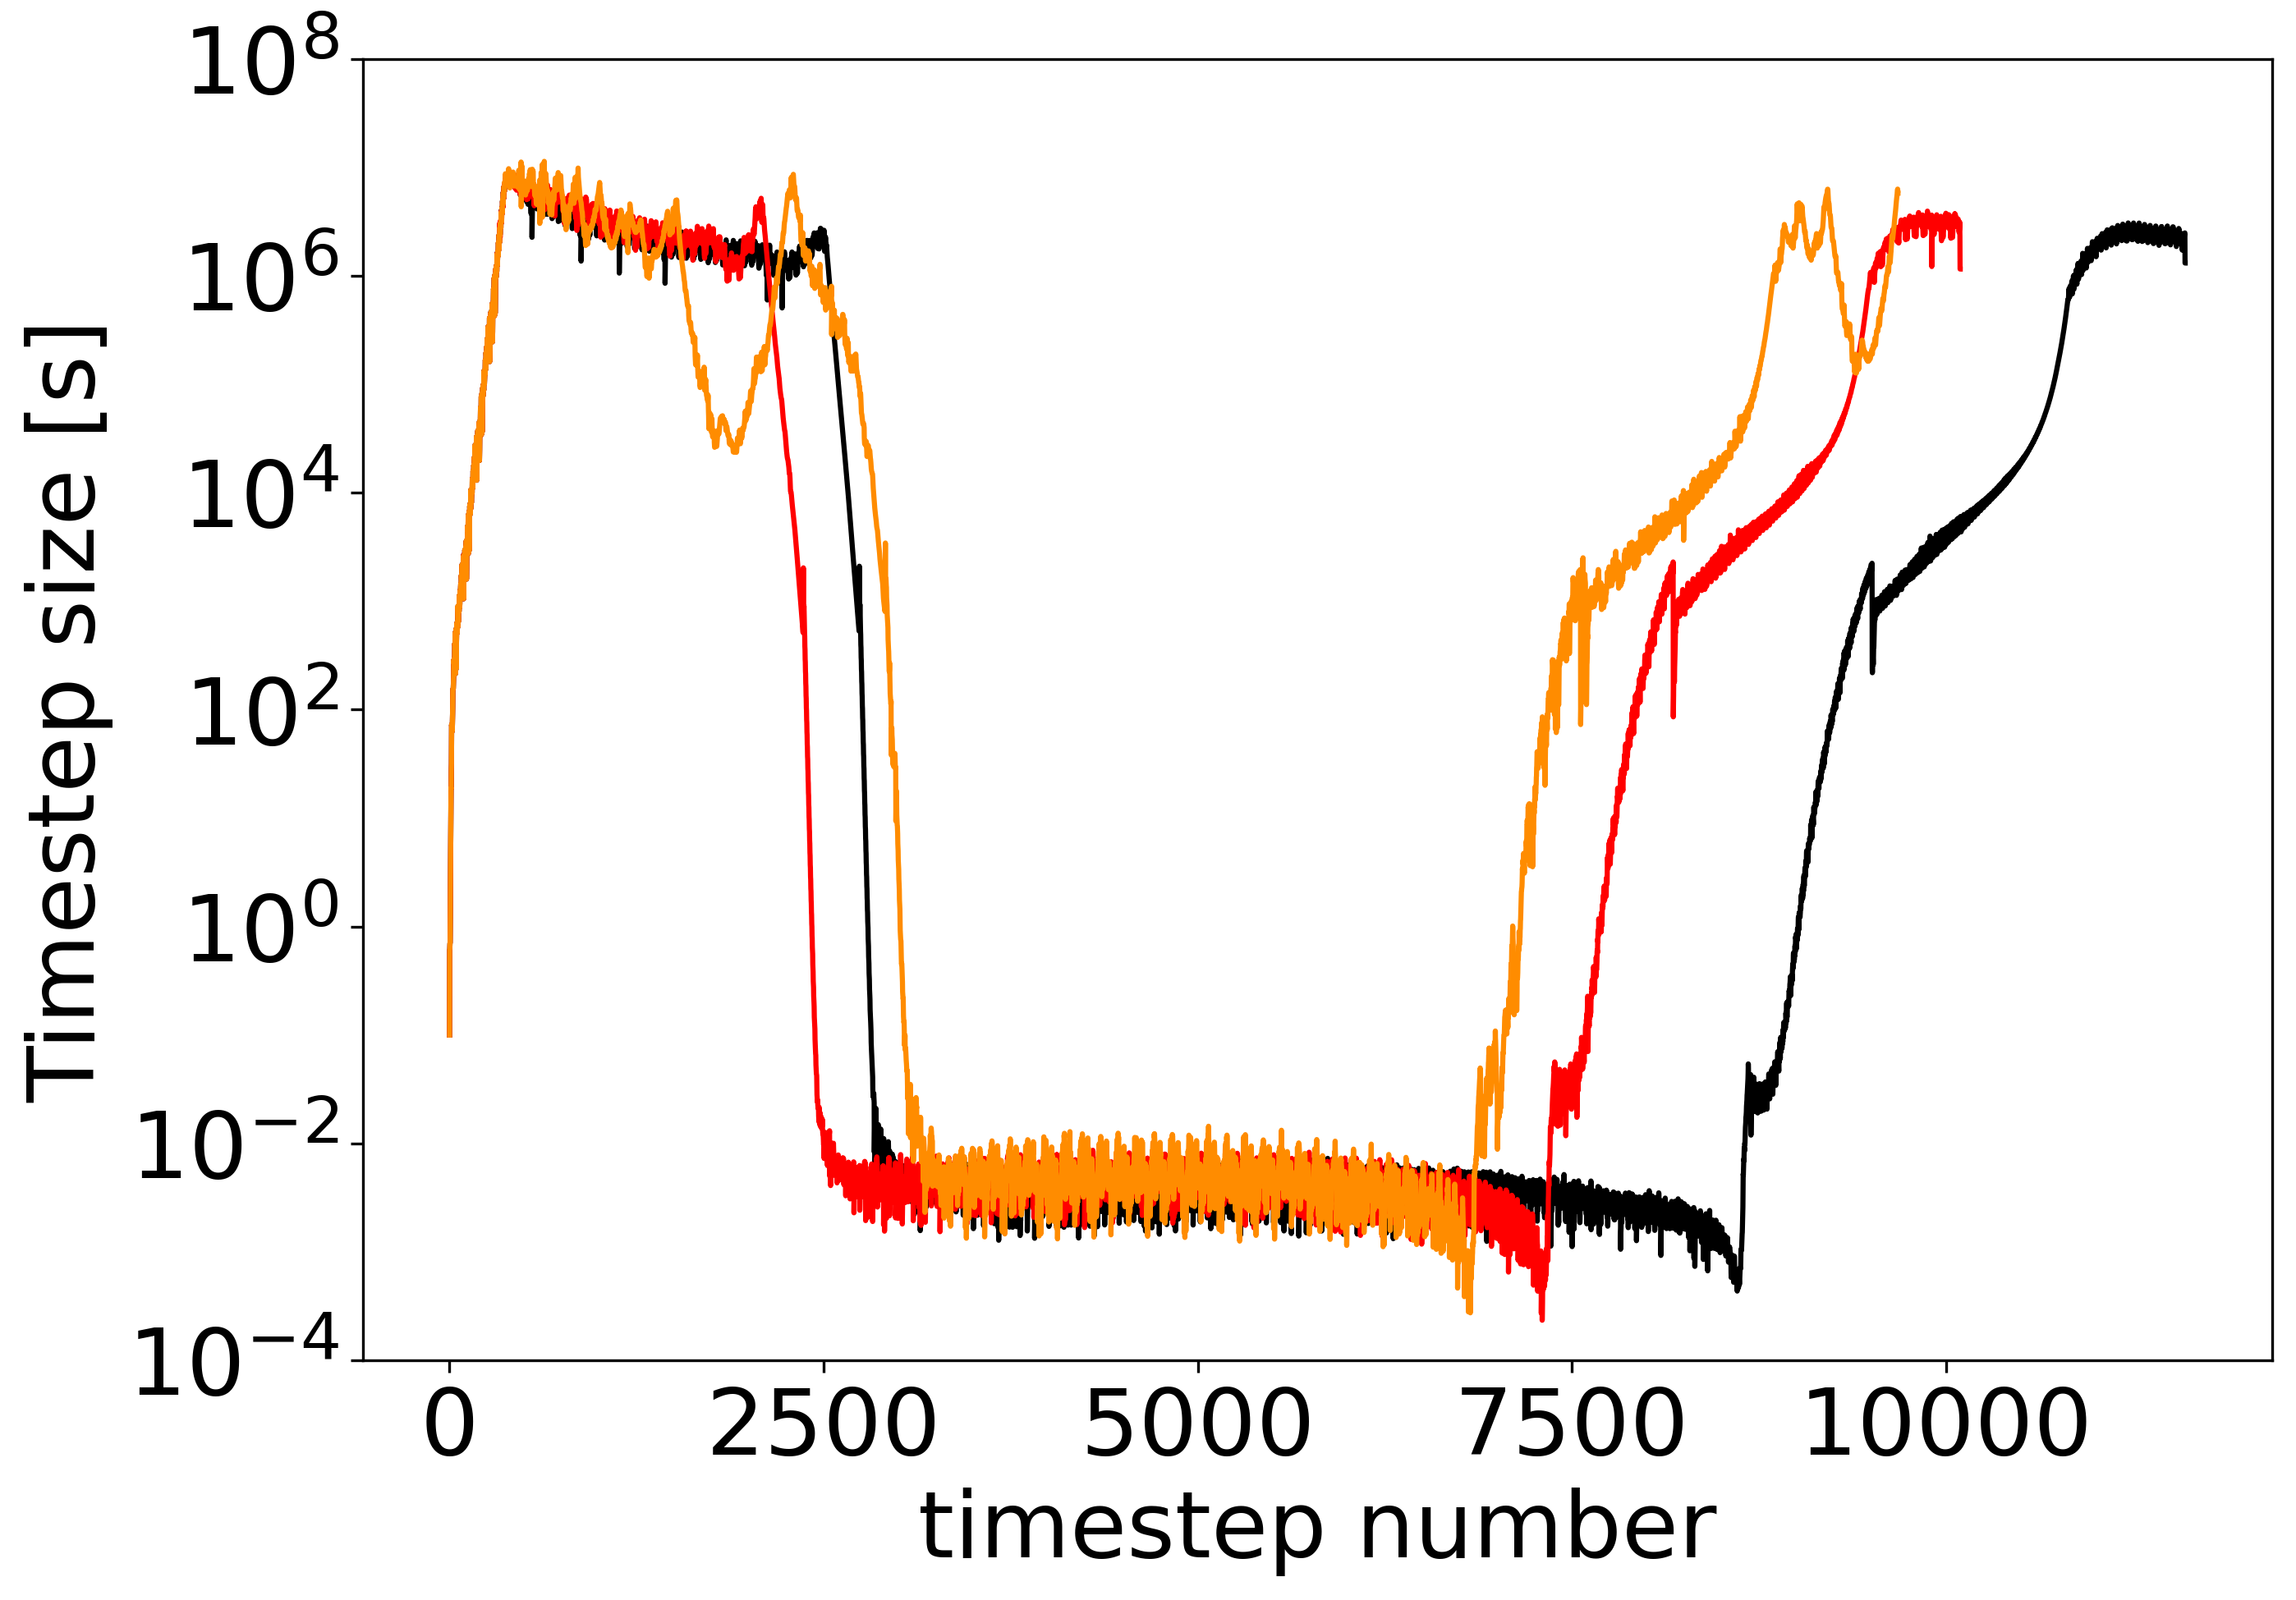
\includegraphics[width=0.99\textwidth]{images/TANDEM_DT_differentSizes_BDFcompactODE.png}
		\subcaption{1st order ODE (BDF) }
	\end{subfigure}
	\begin{subfigure}[b]{0.32\textwidth}
		\centering
		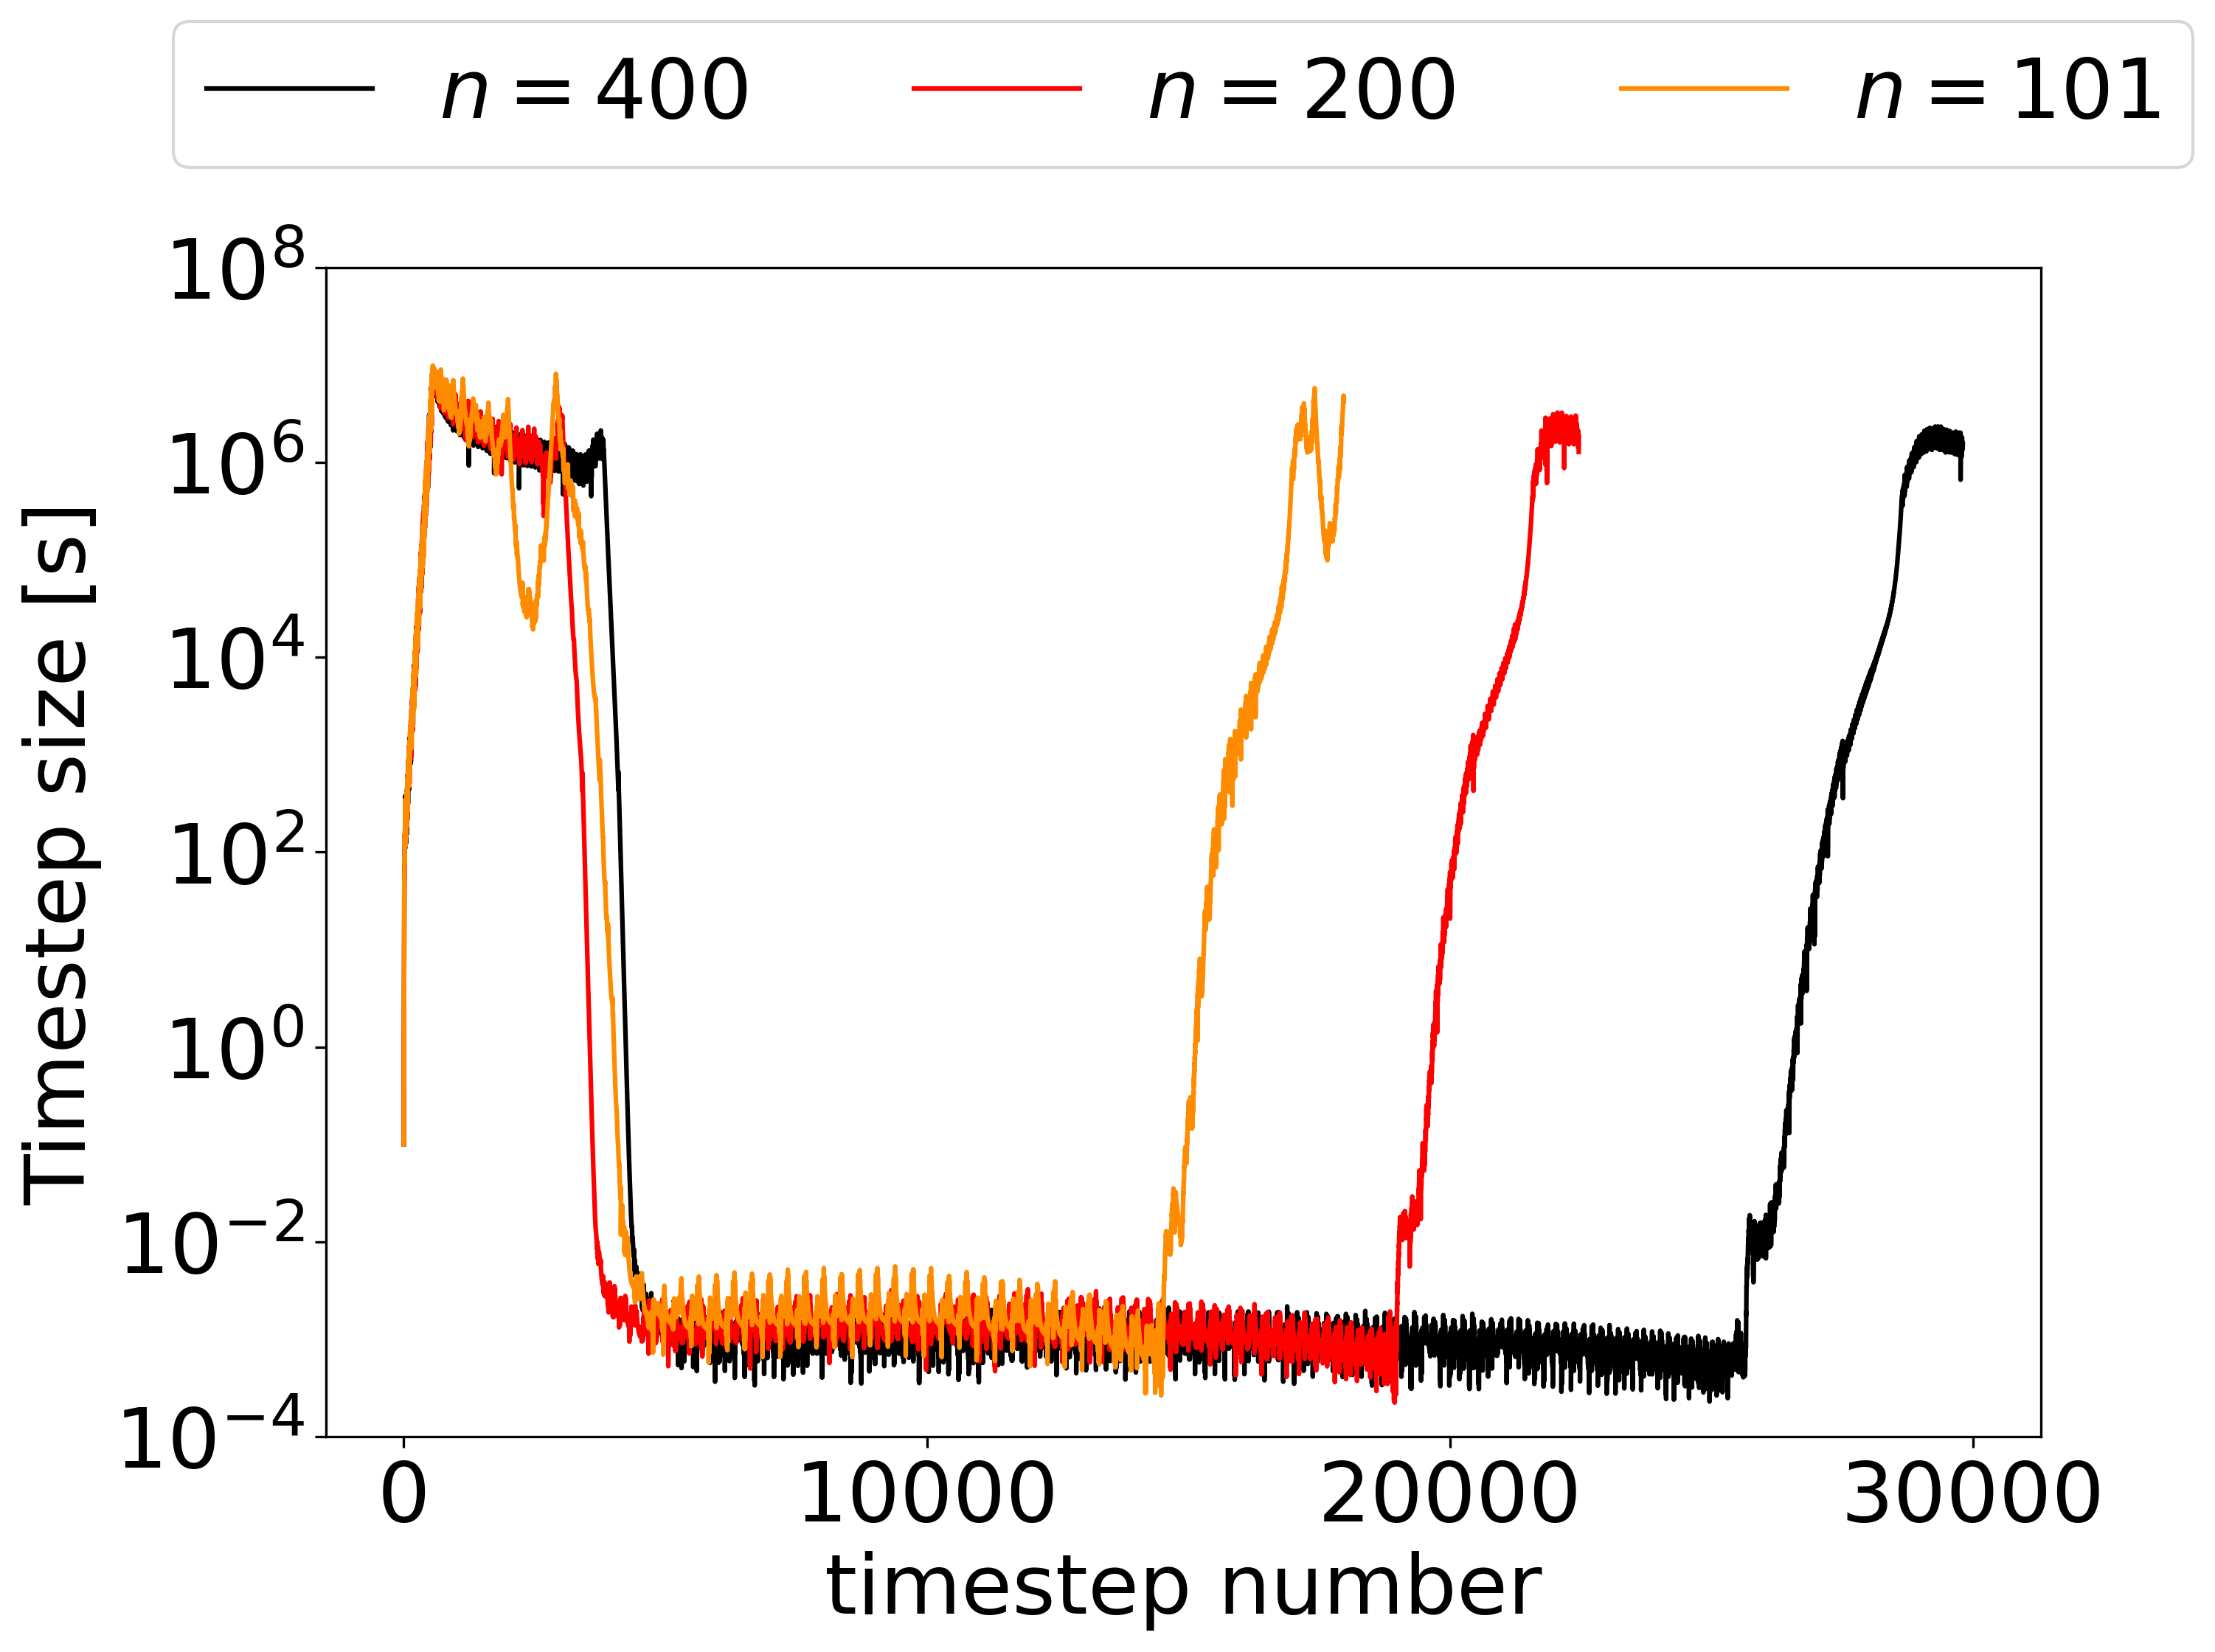
\includegraphics[width=1.04\textwidth]{images/TANDEM_DT_differentSizes_BDFextendedODE.png}
		\subcaption{2nd order ODE (BDF) }
	\end{subfigure}
	\begin{subfigure}[b]{0.32\textwidth}
		\centering
		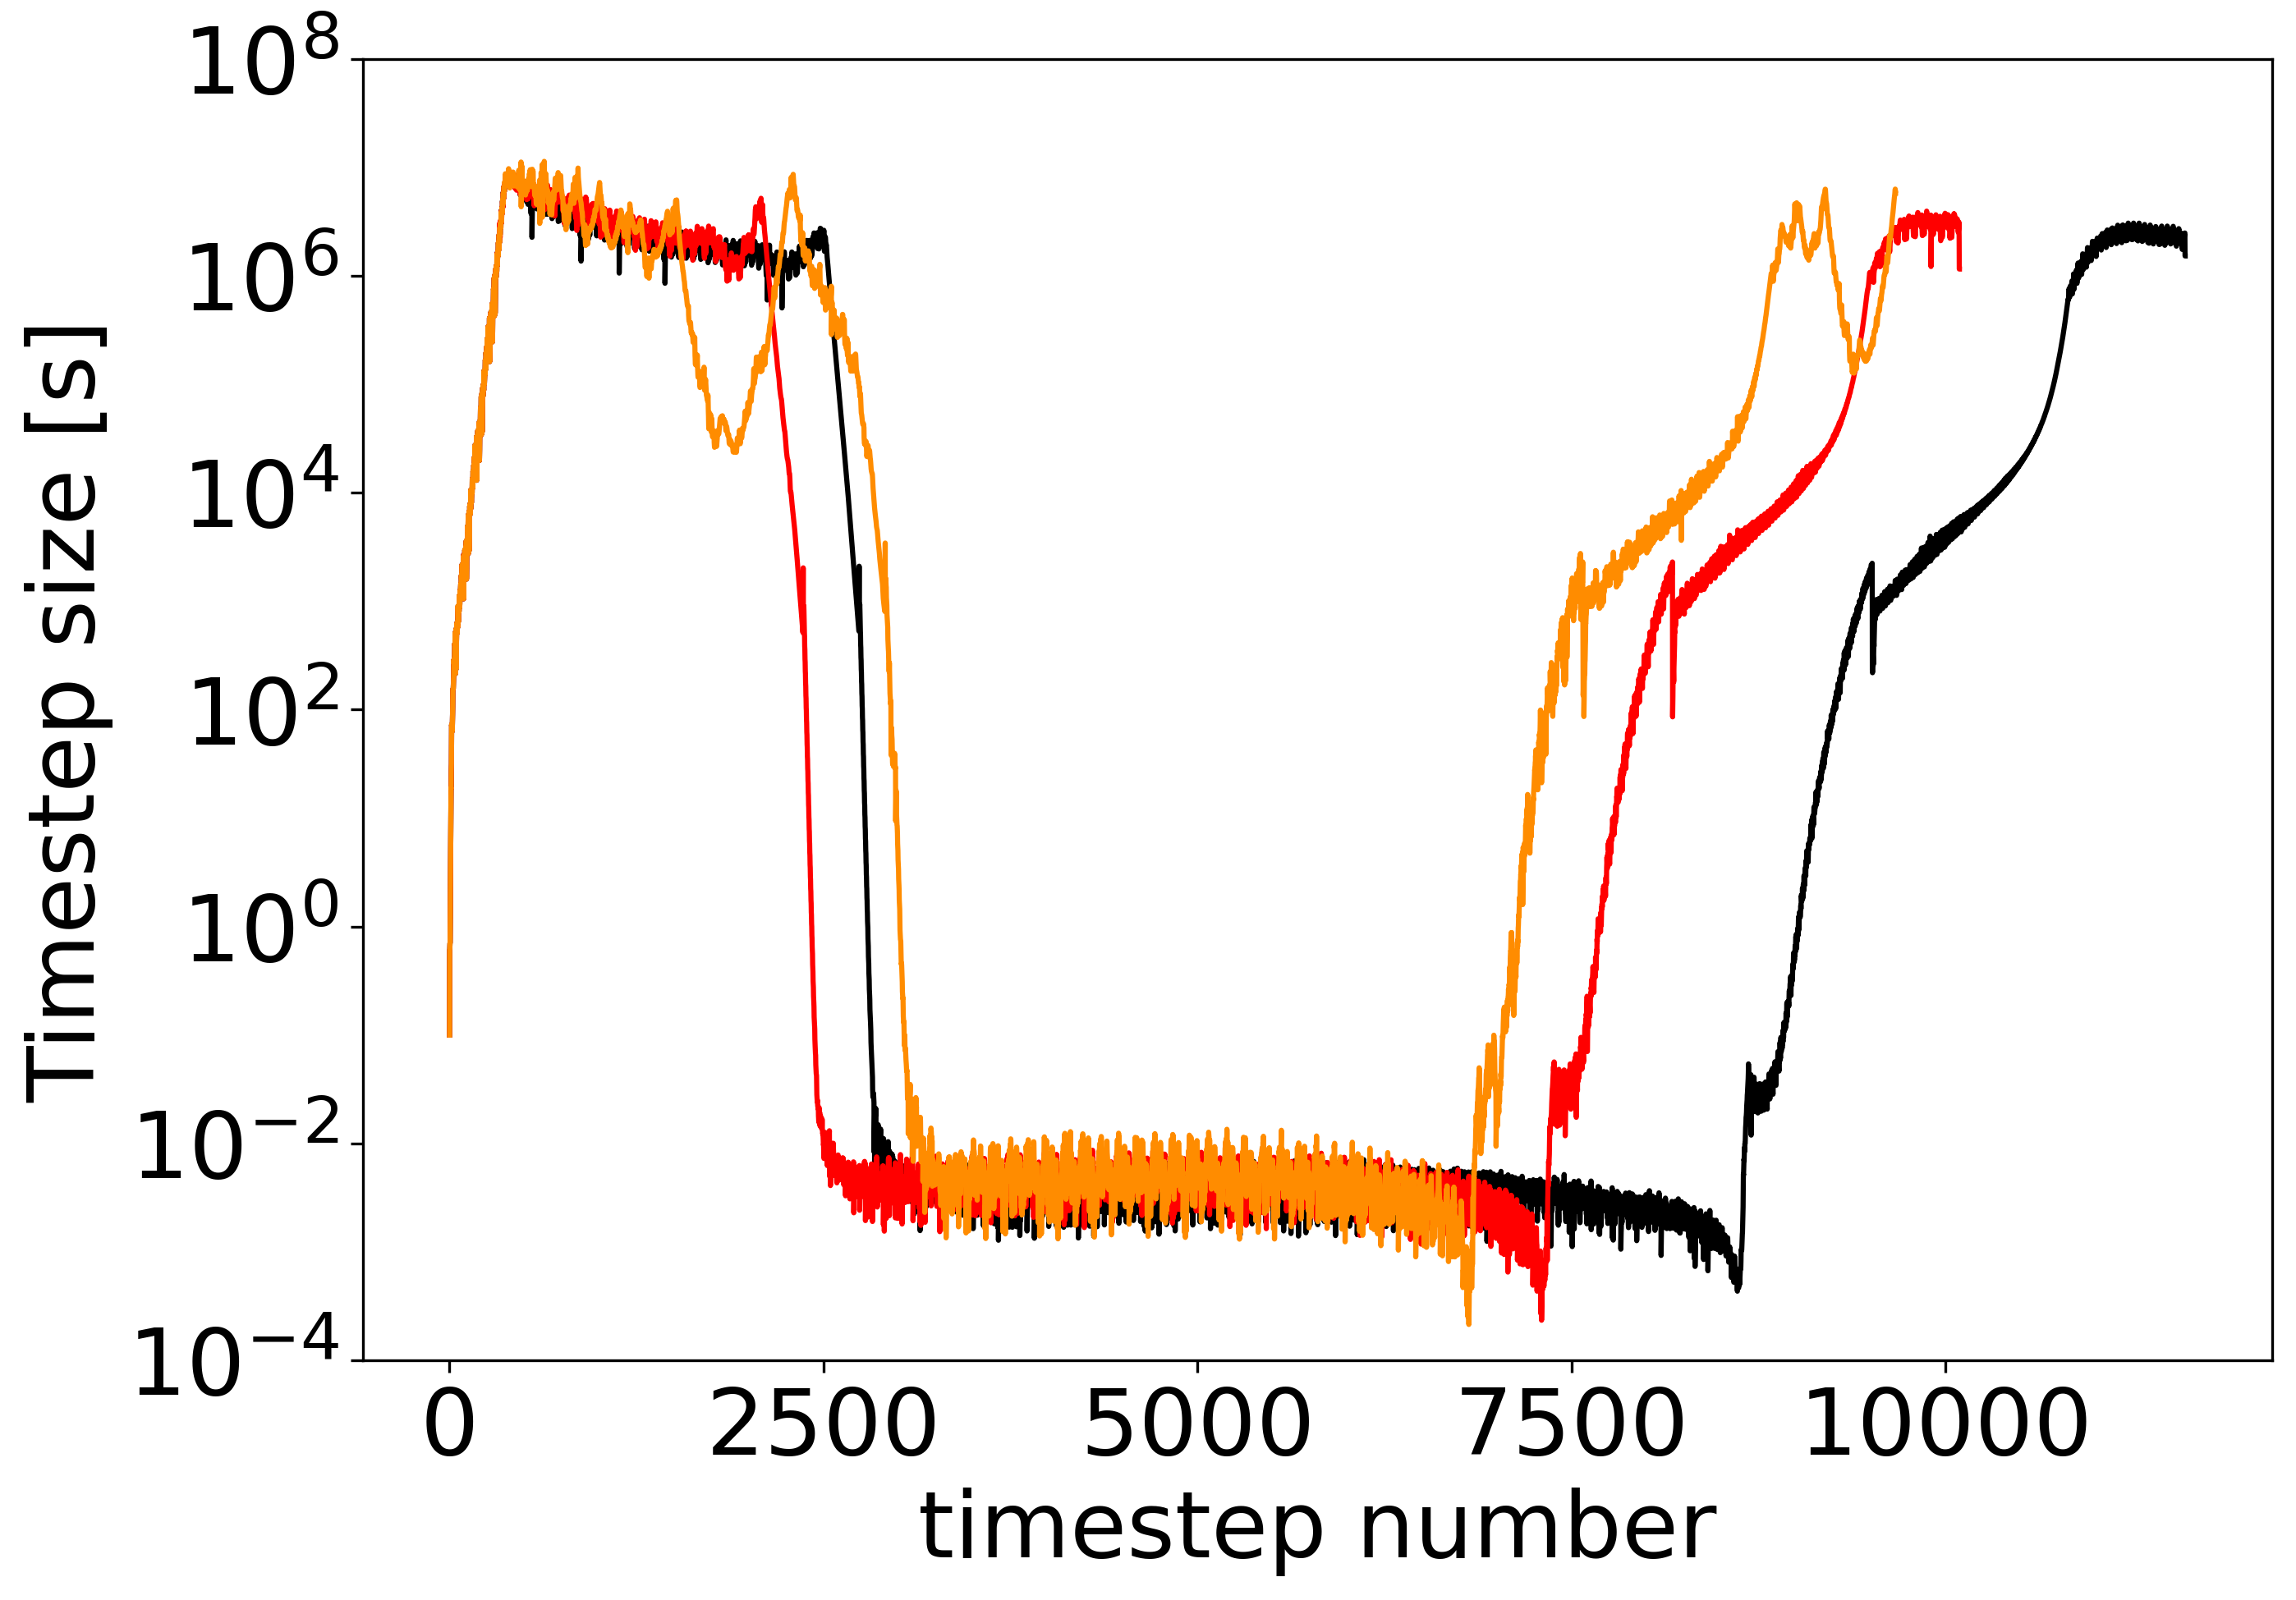
\includegraphics[width=0.99\textwidth]{images/TANDEM_DT_differentSizes_extendedDAE.png}
		\subcaption{extended DAE (BDF) }
	\end{subfigure}
	\begin{subfigure}[b]{0.32\textwidth}
		\centering
		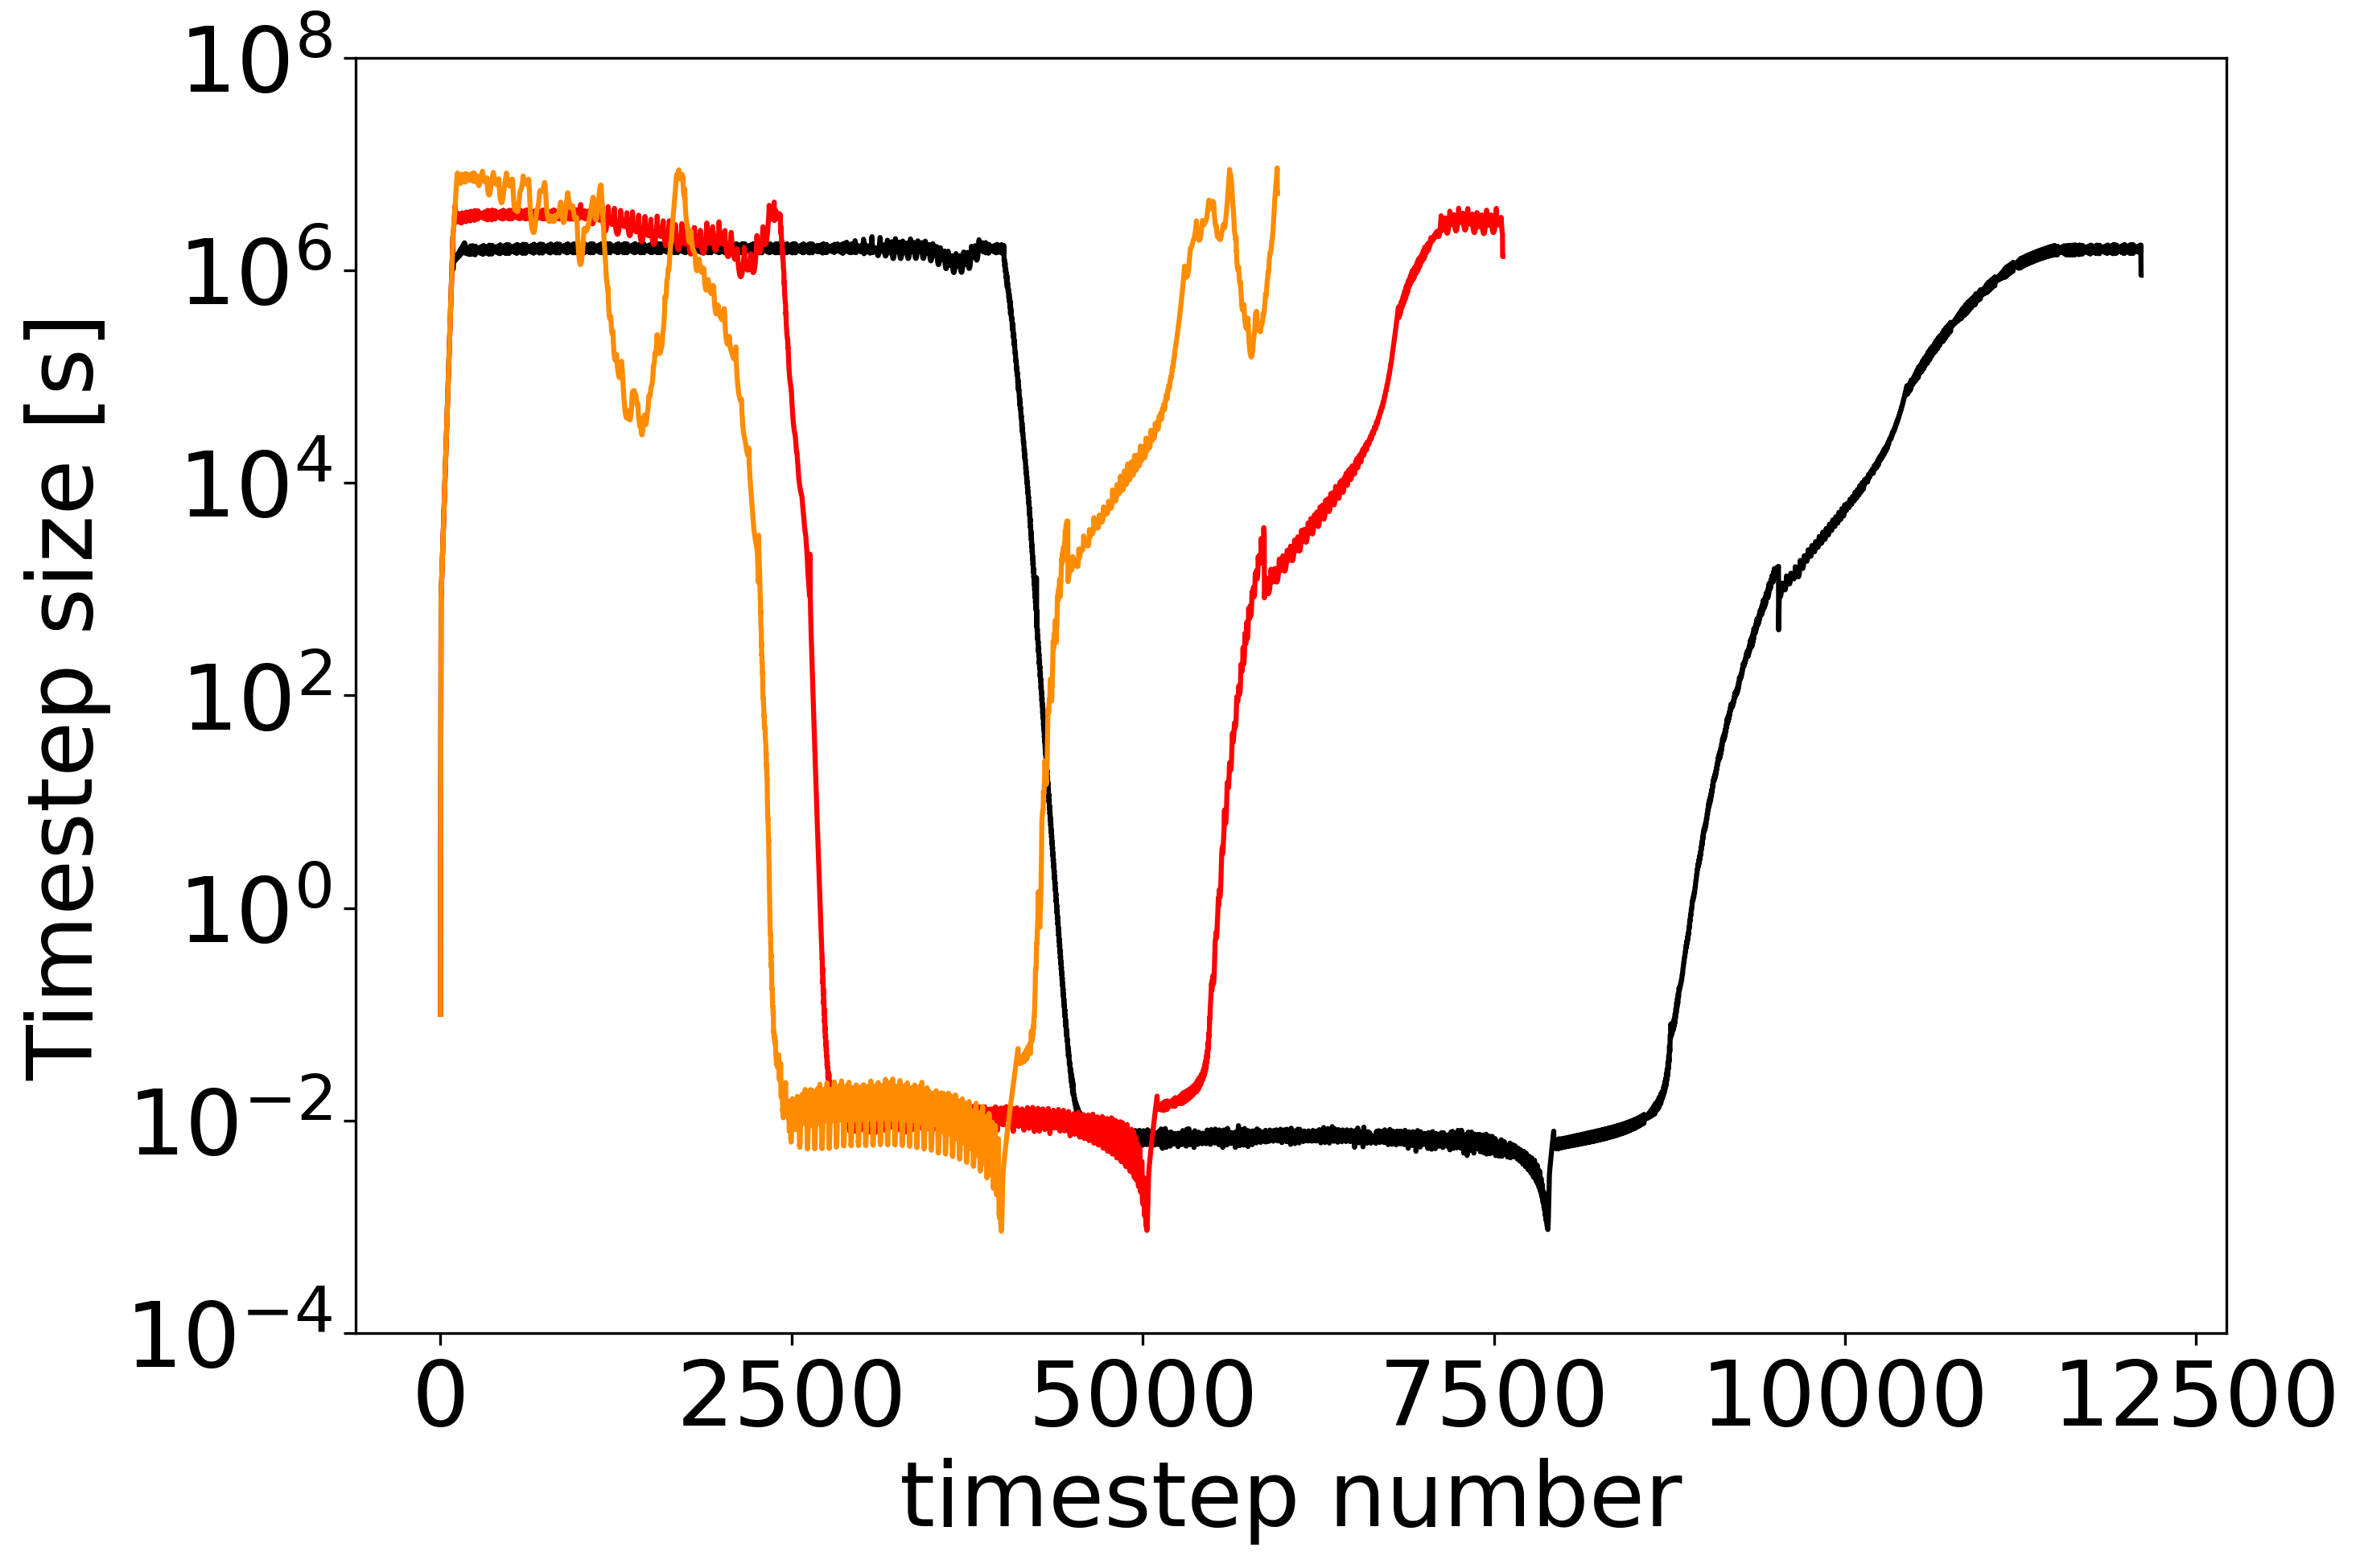
\includegraphics[width=1\textwidth]{images/TANDEM_DT_differentSizes_compactODE.png}
		\subcaption{1st order ODE (RK) }
	\end{subfigure}
	\begin{subfigure}[b]{0.32\textwidth}
		\centering
		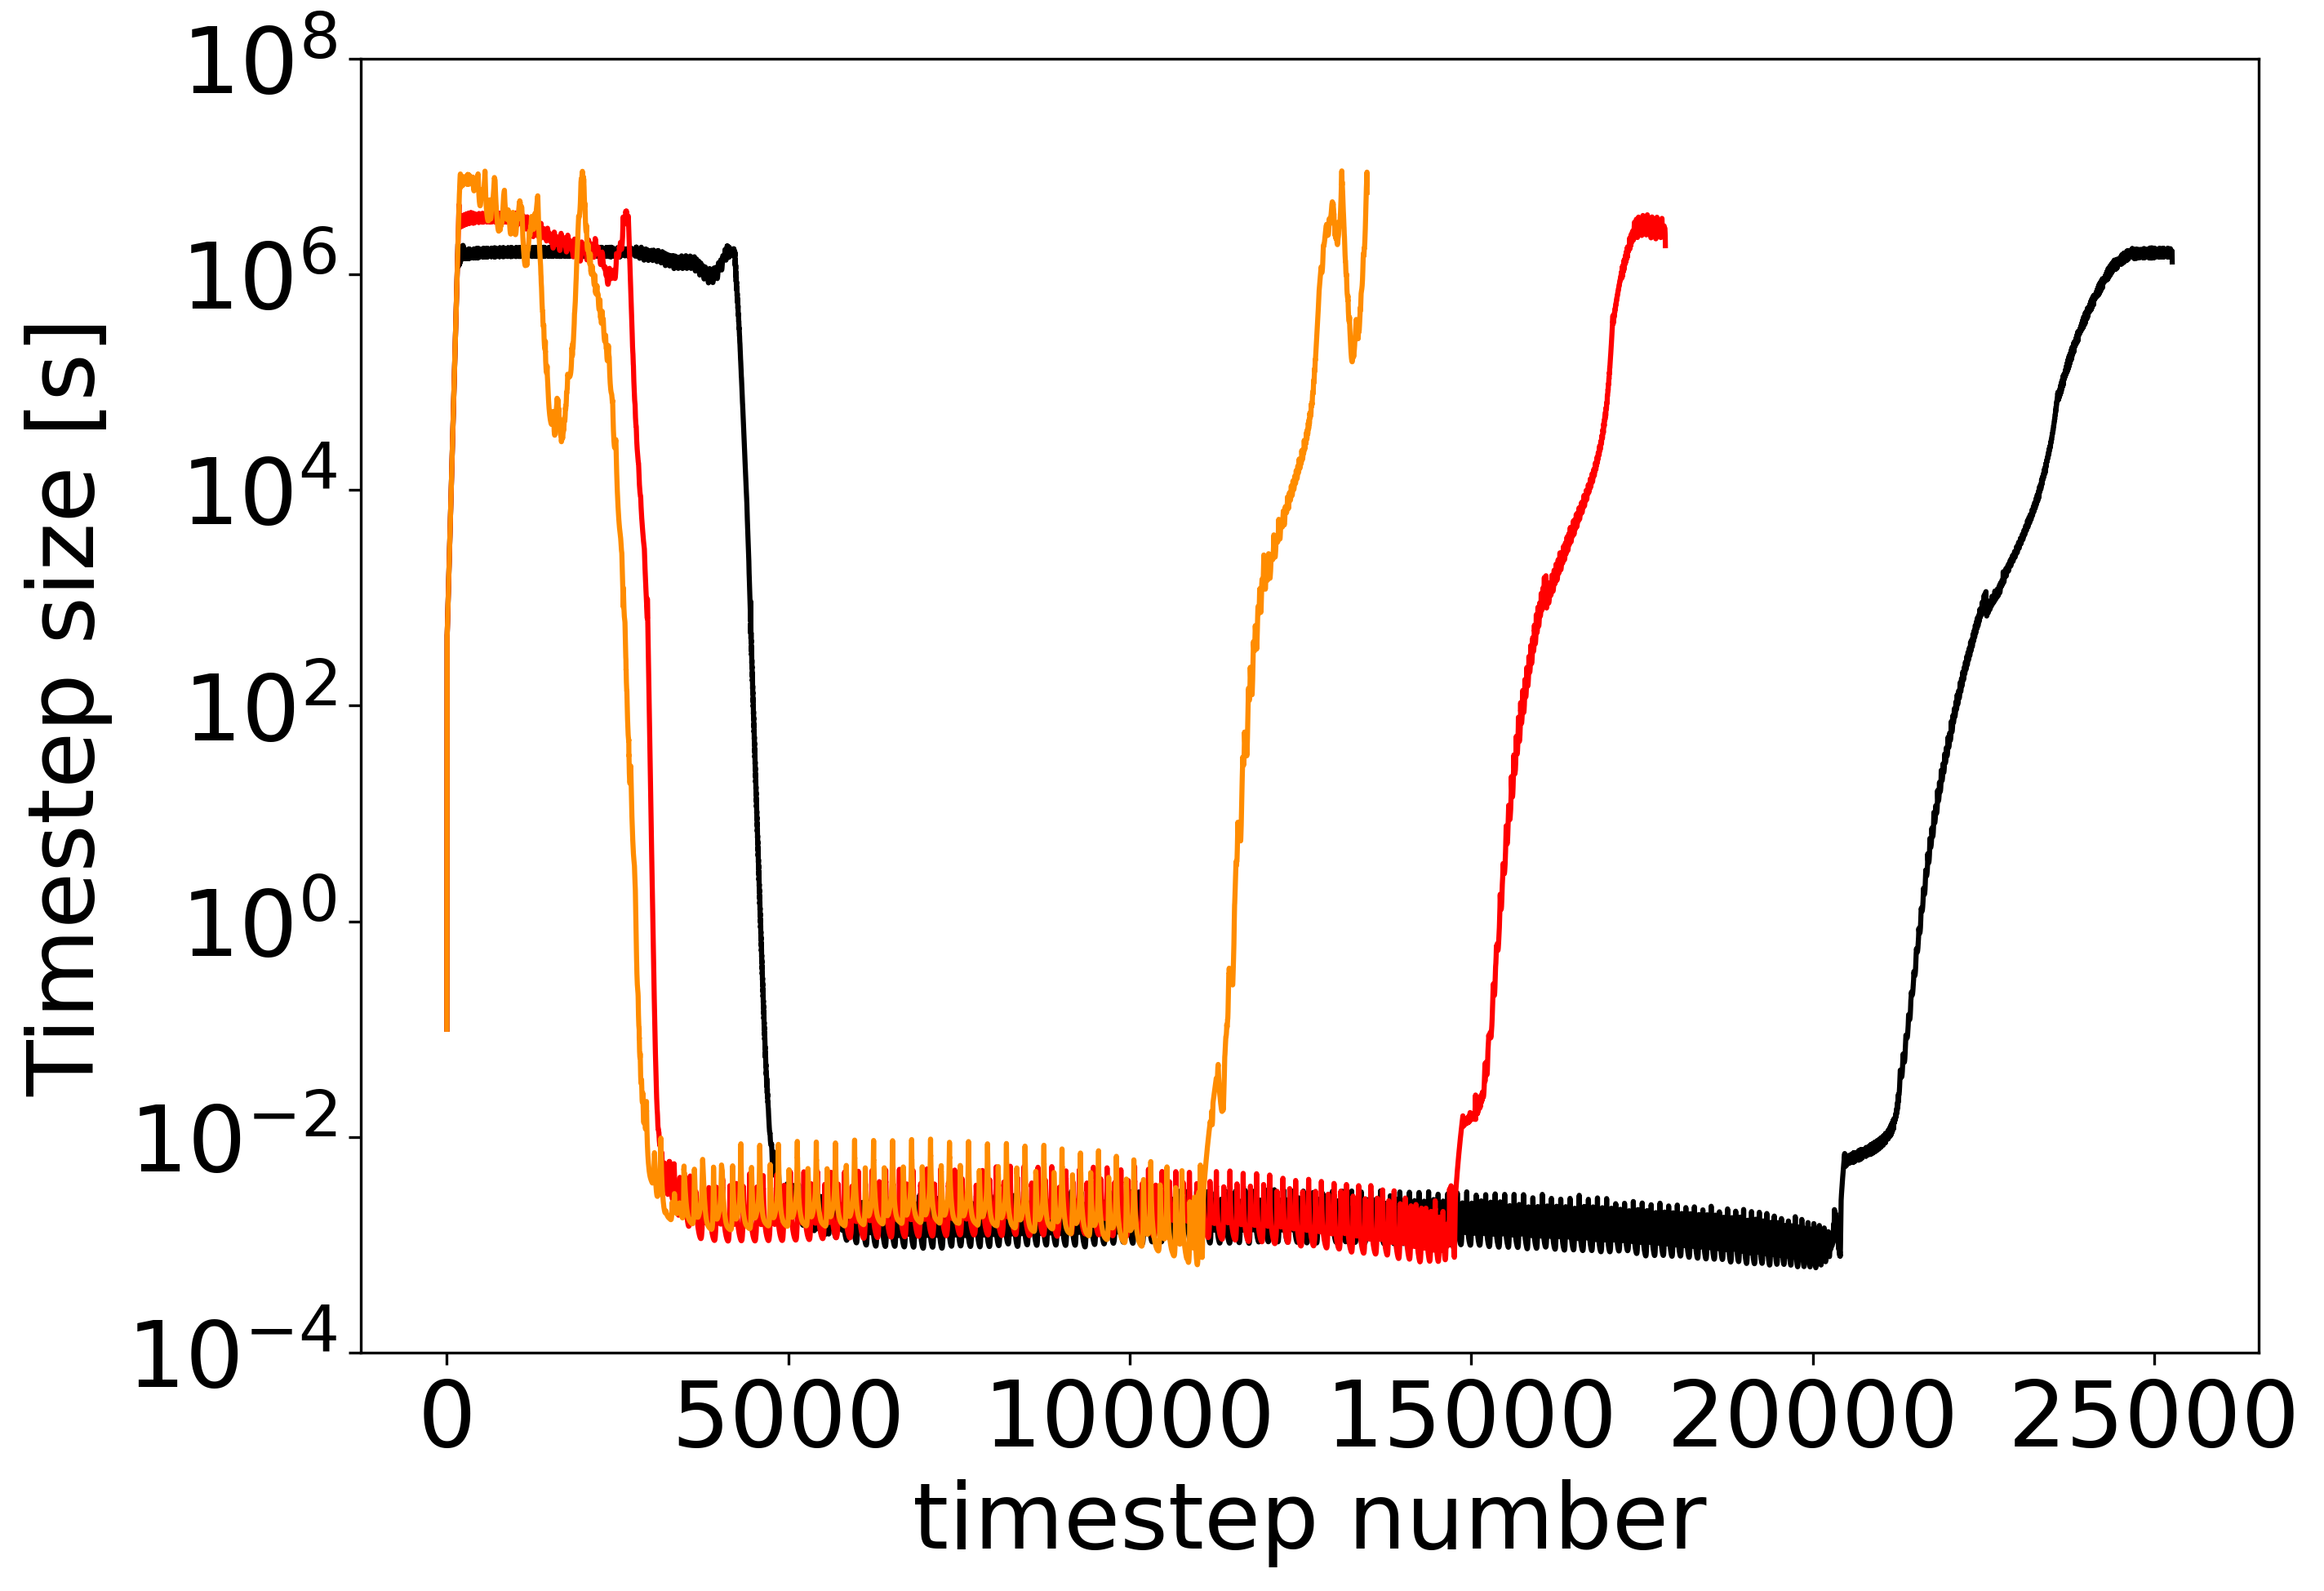
\includegraphics[width=1\textwidth]{images/TANDEM_DT_differentSizes_extendedODE.png}
		\subcaption{2nd order ODE (RK) }
	\end{subfigure}
	\begin{subfigure}[b]{0.32\textwidth}
		\centering
		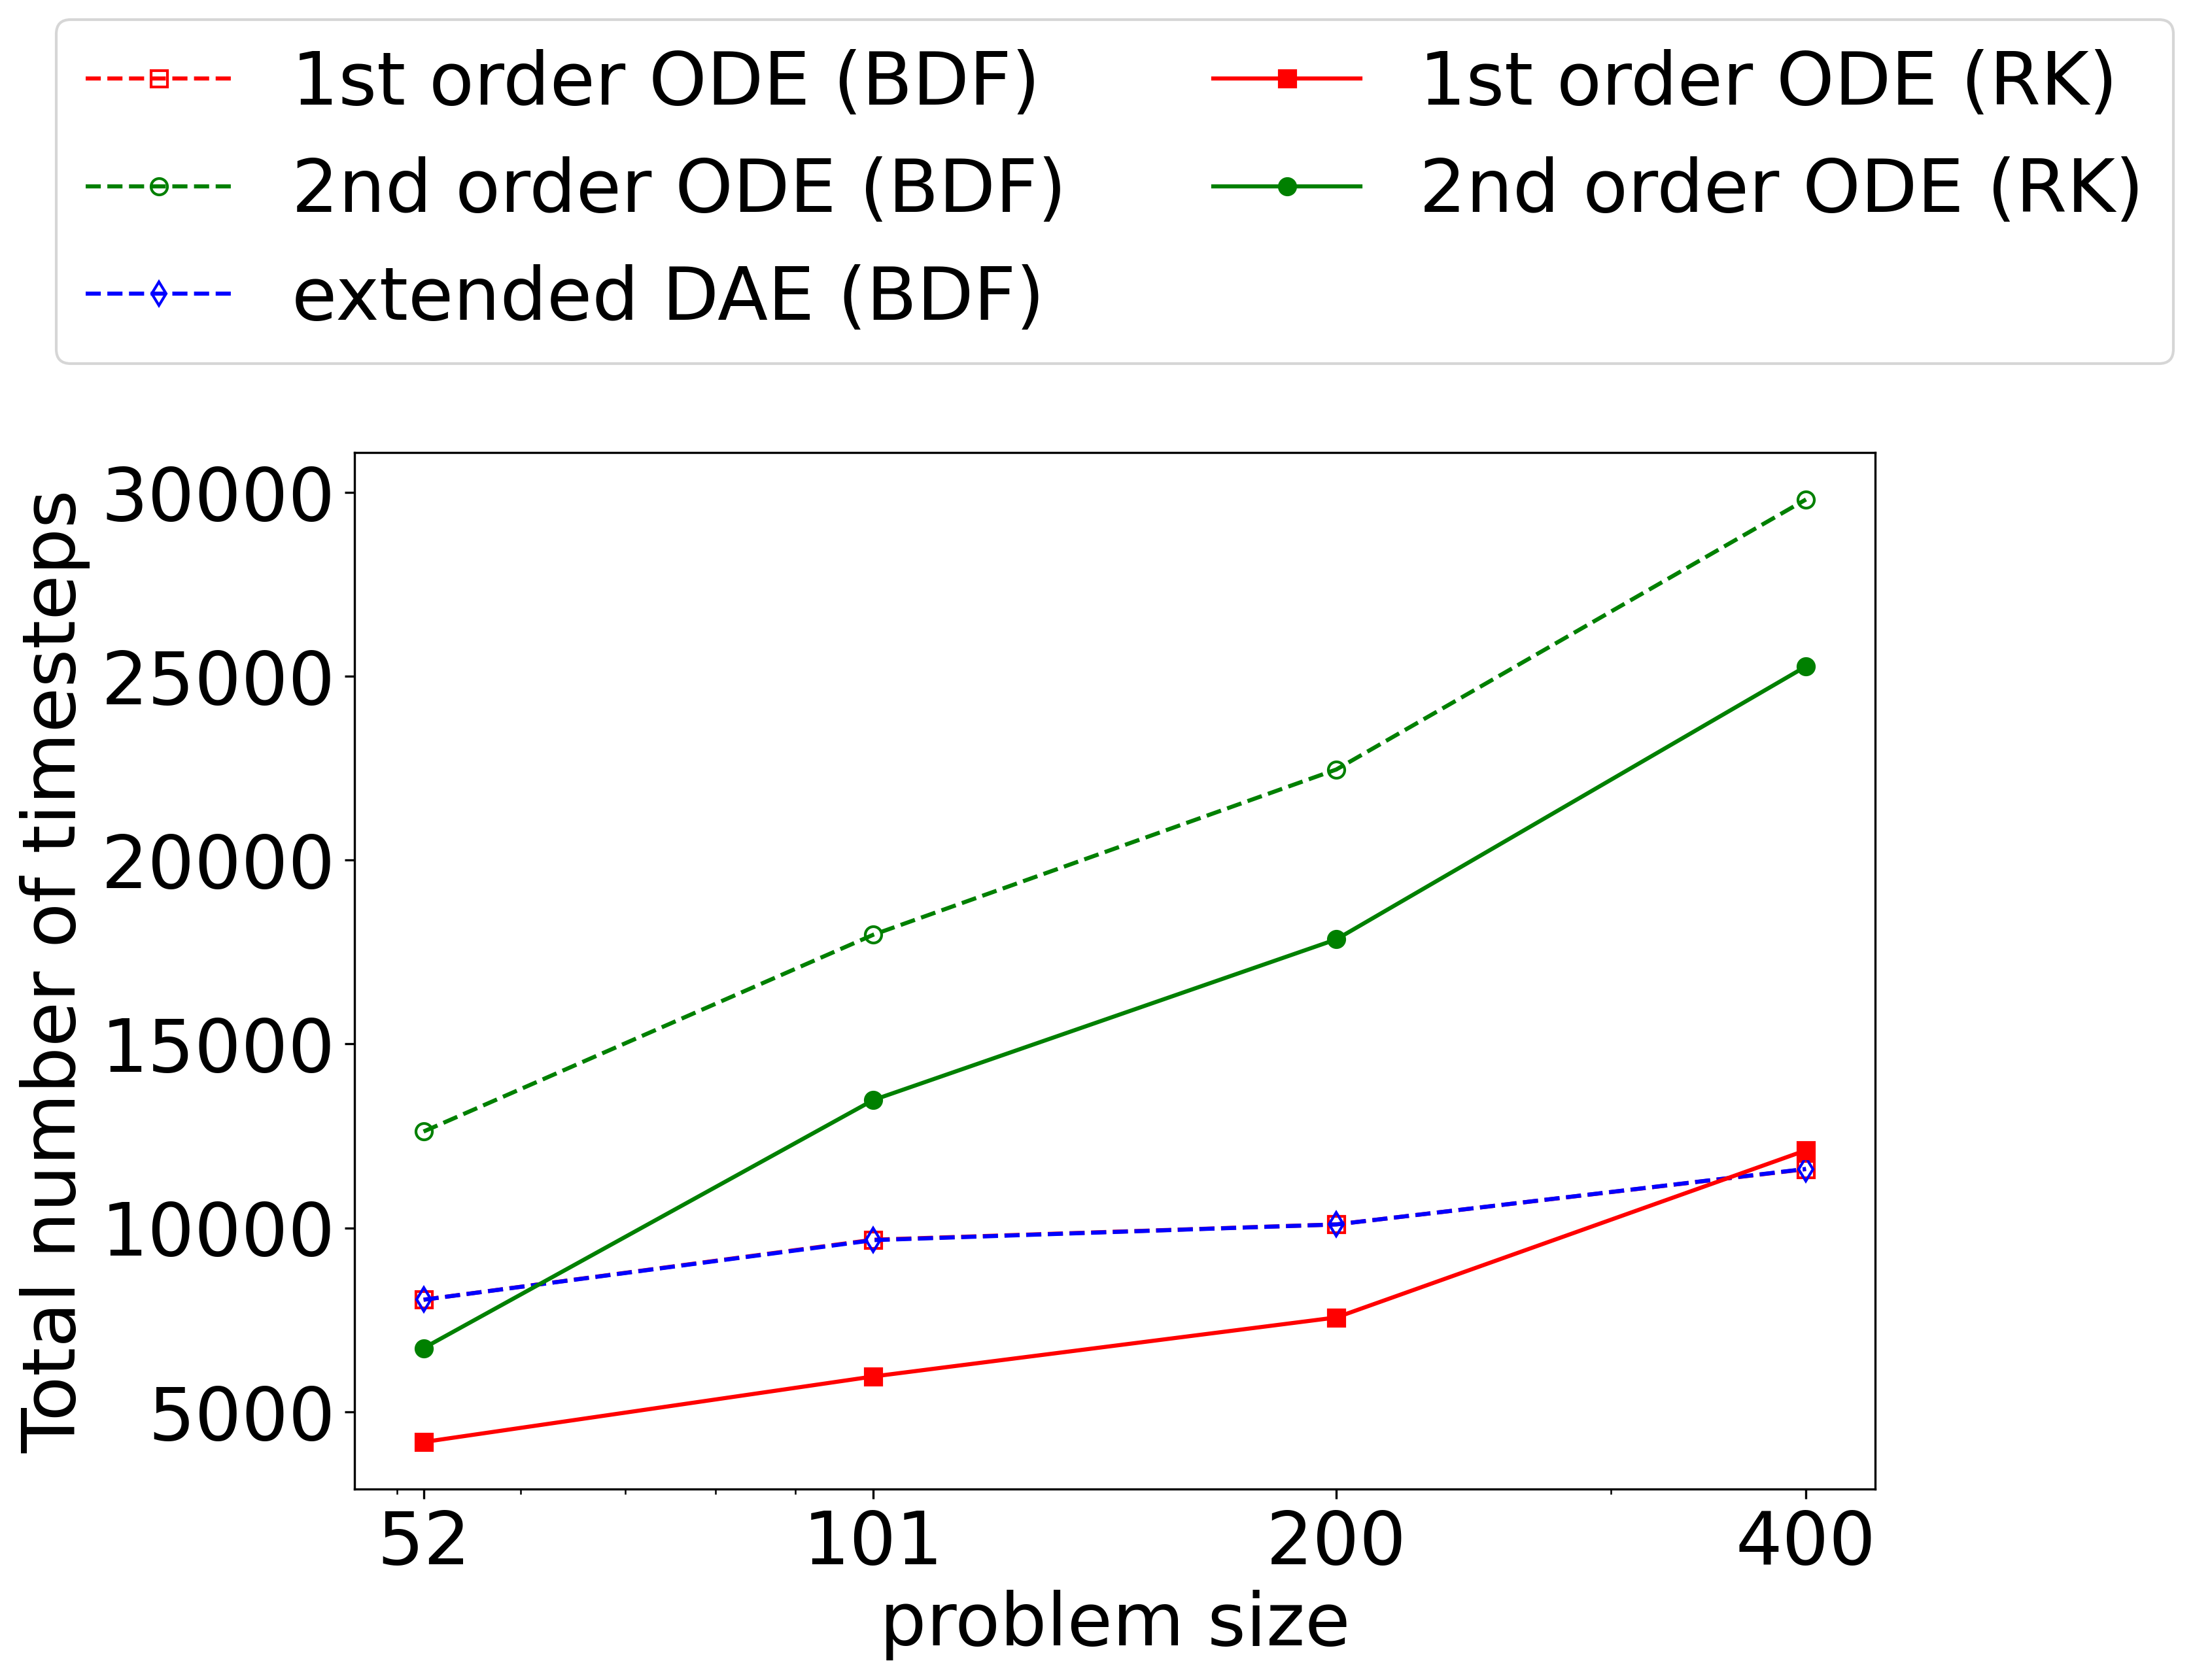
\includegraphics[width=1.14\textwidth]{images/TANDEM_NumberTimeSteps_differentSizes.png}
		\subcaption{Total number of timesteps }
	\end{subfigure}
	\caption{Evolution of the timestep size over the whole simulation for each combination of formulation and time integration method on different problem sizes.}
	\label{fig:scalabilty_timeStepSizes}
\end{figure}
The most obvious observation is that the second order ODE formulation requires considerably more timesteps than the first order formulations. For instance in the earthquake phase, the timestep size varies between $h=10^{-4}$s and $10^{-3}$s for the former as opposed to the range between $h=10^{-3}$s and $10^{-2}$s for the latter. This result was quite expected, as a higher order ODE is naturally less accurate and only allows for smaller timesteps to match the prescribed tolerance. Much more interesting is that the timestep size is almost not affected by the domain size for the two implicit 1st order schemes in graphs (a) and (c). Actually, both formulations produce almost identical timestep sizes, so that the total number of timesteps cannot be distinguished in the last graph. For the explicit first order ODE in (d), it can be clearly seen that in the initial aseismic phase, the larger domains produce smaller timesteps and the earthquake phase requires more timesteps to complete. On the other hand, for the two implicit methods, all curves overlap much better initially and the length difference in the earthquake phase is much less extreme. For the 2nd order formulation, this advantage of the implicit scheme in (b) over the explicit scheme in (e) only appears in the aseismic phase where the timestep sizes overlap, but the length of the earthquake phase increases similarly with the domain size. Graph (f) confirms these observations: all formulations suffer an important increase in the total number of timesteps except for the implicit extended DAE and the implicit 1st order ODE formulations. Supposing that this trend continues if the domain size is further increased, only these two approaches are competitive.


\subsection{Execution times}
The total number of timesteps is a good indicator of the scalability of a formulation, but is not as well suited to directly compare formulations. Indeed the effort to perform one timestep varies greatly: all 1st order formulations have to solve the DG problem, instead of the 2nd order ODE formulation only needs a matrix-vector multiplication to calculate the RHS; the 1st order ODE formulation includes a nonlinear solver in the RHS for the slip rate, the other formulations do not; implicit methods need to set up the Jacobian matrix at each Newton step and the convergence speed of the Newton and GMRES iterations depends on the problem size and the formulation, as it was already discussed in \autoref{ssec_Results_Scalability_IterativeSchemes}. Further, the explicit 1st order ODE formulation is the only approach that does not require precomputing constant Jacobian matrices in the initialization phase, which takes a considerable amount of time for large times. All in all, the computational effort per timestep depends strongly on the chosen combination between formulation and time integration method. To evaluate this effort and compare the possible approaches, the CPU time, or wall clock time since the program is entirely sequential, has been measured. As the measurements were only done once on a personal computer with high-priority processes, the results come along with high uncertainty but are sufficiently accurate to distinguish the trend of the computational effort. The average execution time of a RHS evaluation is compared in \autoref{fig:scalabilty_executionTimes__timePerStep}, the effort of the initialization phase is shown in \autoref{fig:scalabilty_executionTimes__initializationTime} and the total time spent in the solving phase is found in \autoref{fig:scalabilty_executionTimes__solveTime}.

\begin{figure}[H]
	\centering
	\begin{subfigure}[b]{0.32\textwidth}
		\centering
		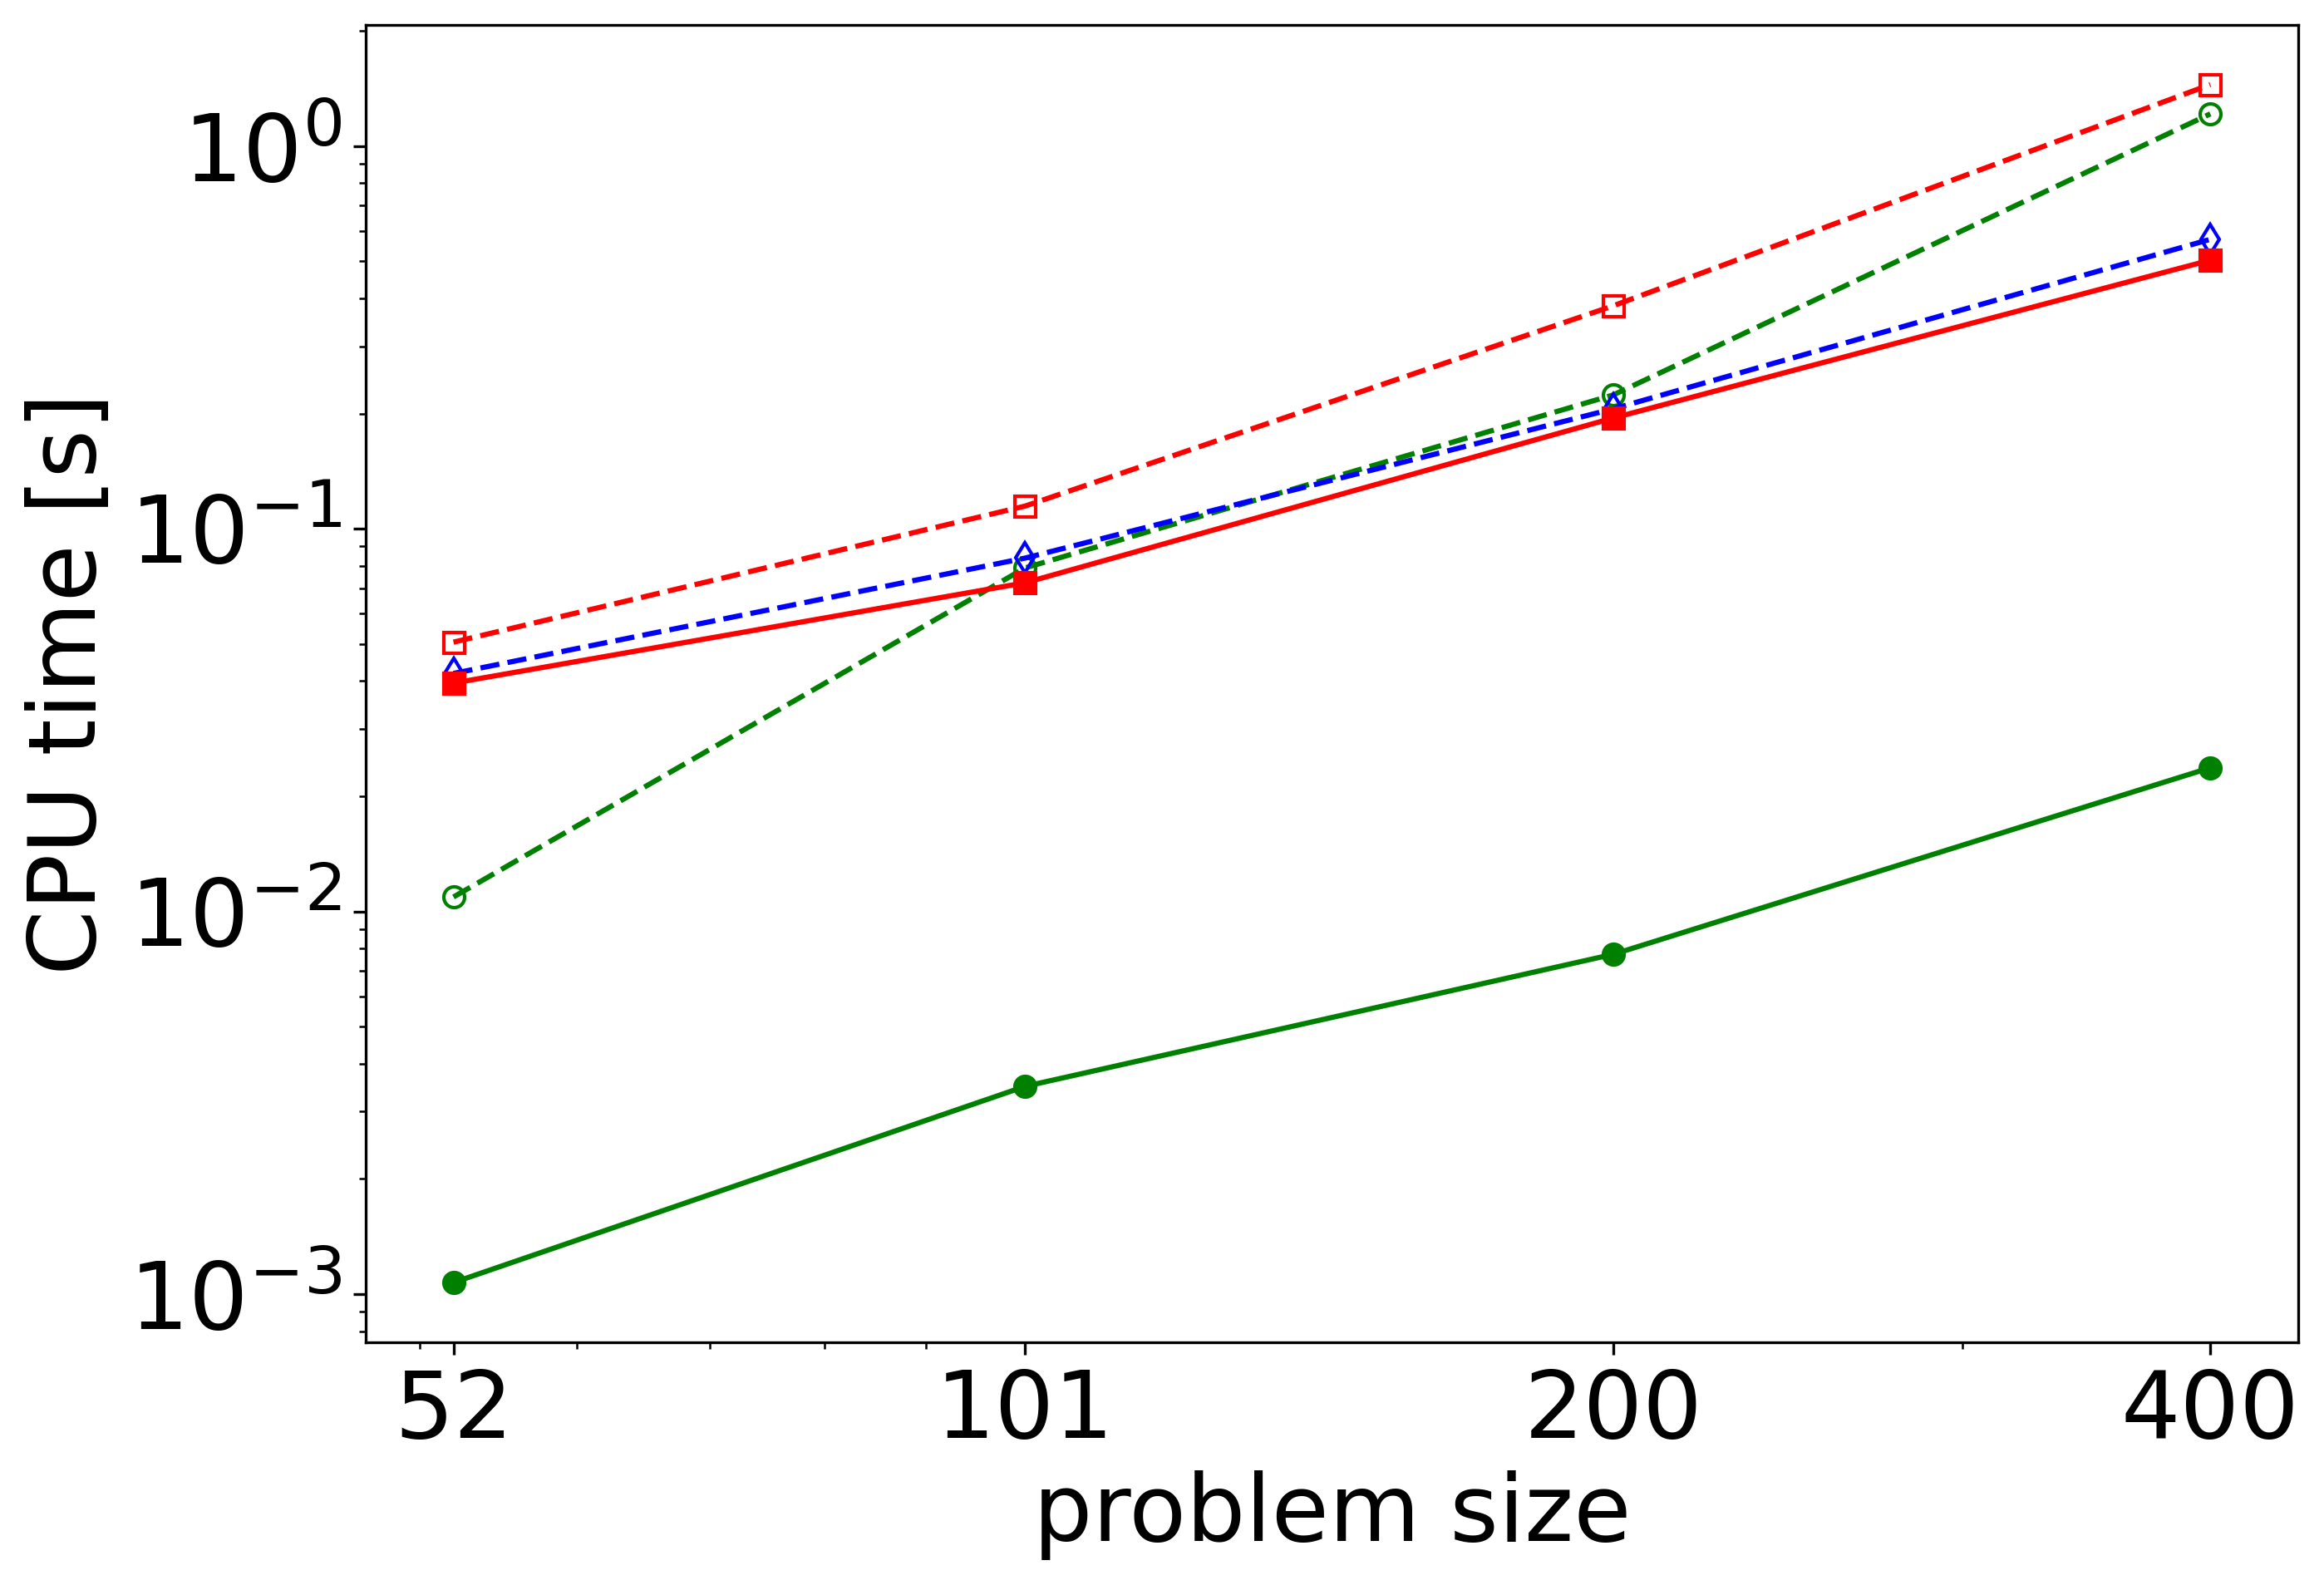
\includegraphics[width=1\textwidth]{images/TANDEM_TimePerRHSEvaluation_differentSizes.png}
		\subcaption{Average execution time \\ of each RHS evaluation}
		\label{fig:scalabilty_executionTimes__timePerStep}
	\end{subfigure}
	\begin{subfigure}[b]{0.32\textwidth}
		\centering \hspace{-0.75cm}
		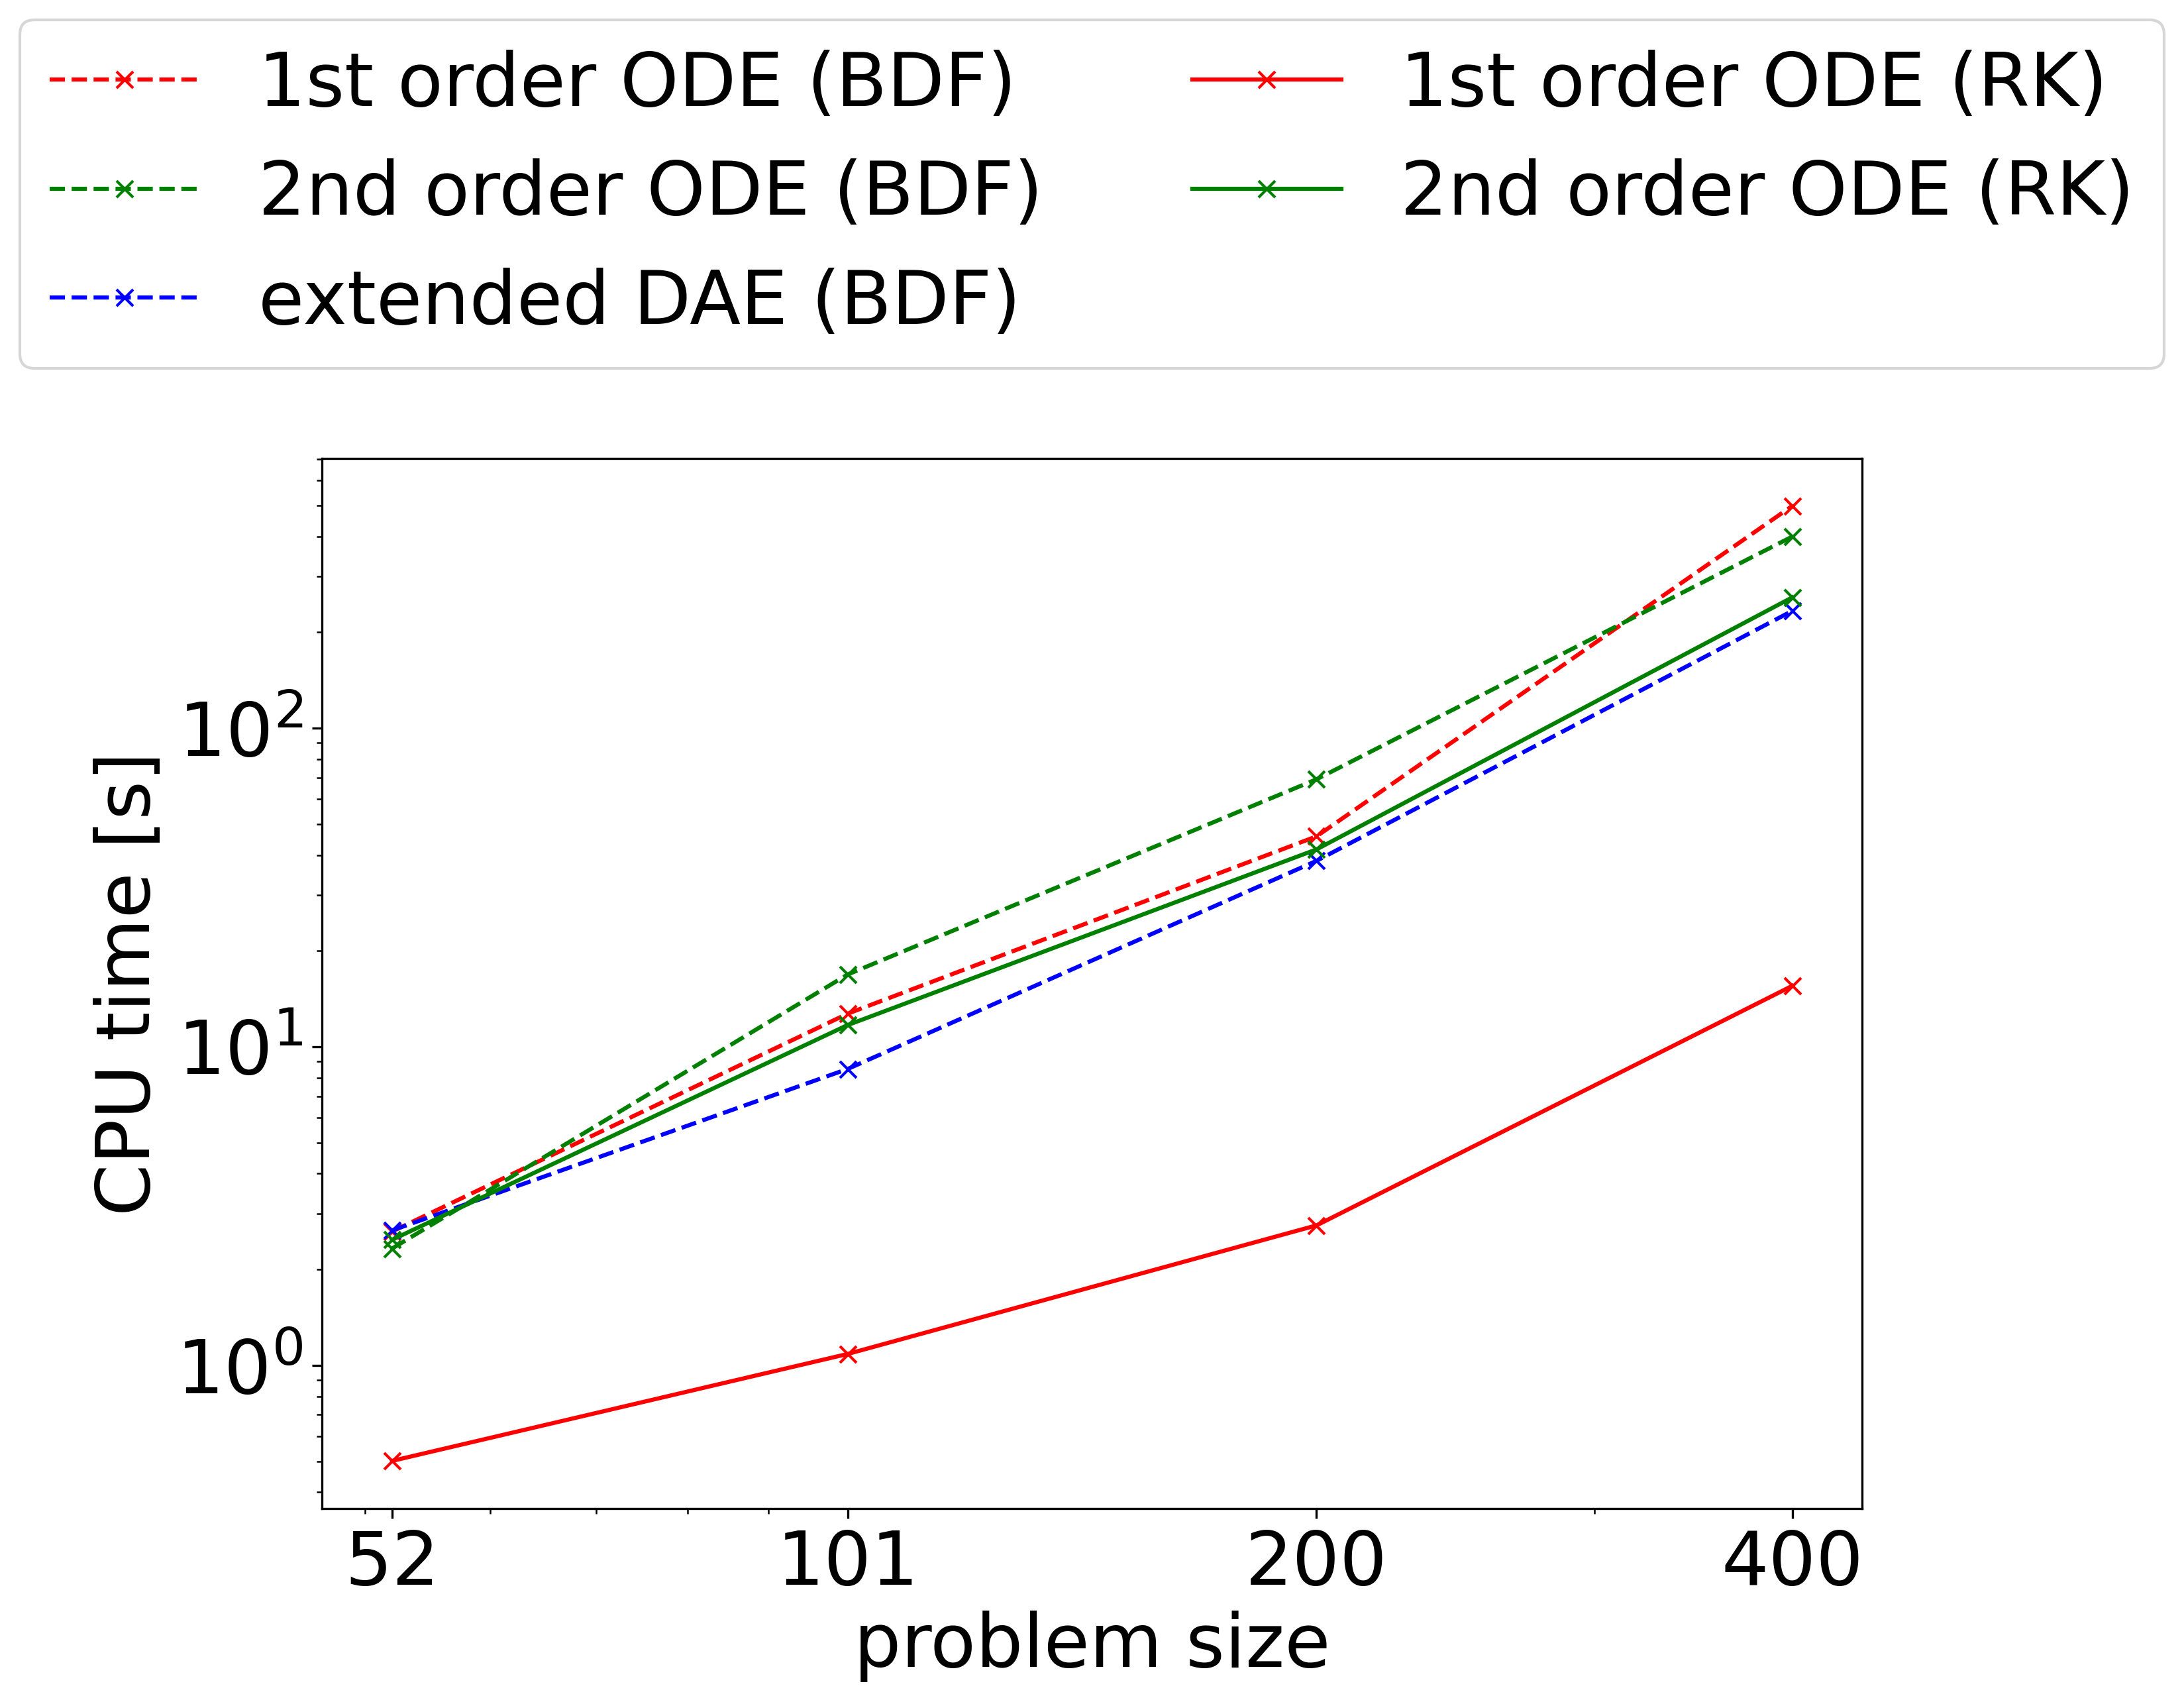
\includegraphics[width=1.18\textwidth]{images/TANDEM_CPU_Time_intialization.png}
		\subcaption{Execution time of the \\ initialization phase} 
		\label{fig:scalabilty_executionTimes__initializationTime}
	\end{subfigure}
	\begin{subfigure}[b]{0.32\textwidth}
		\centering
		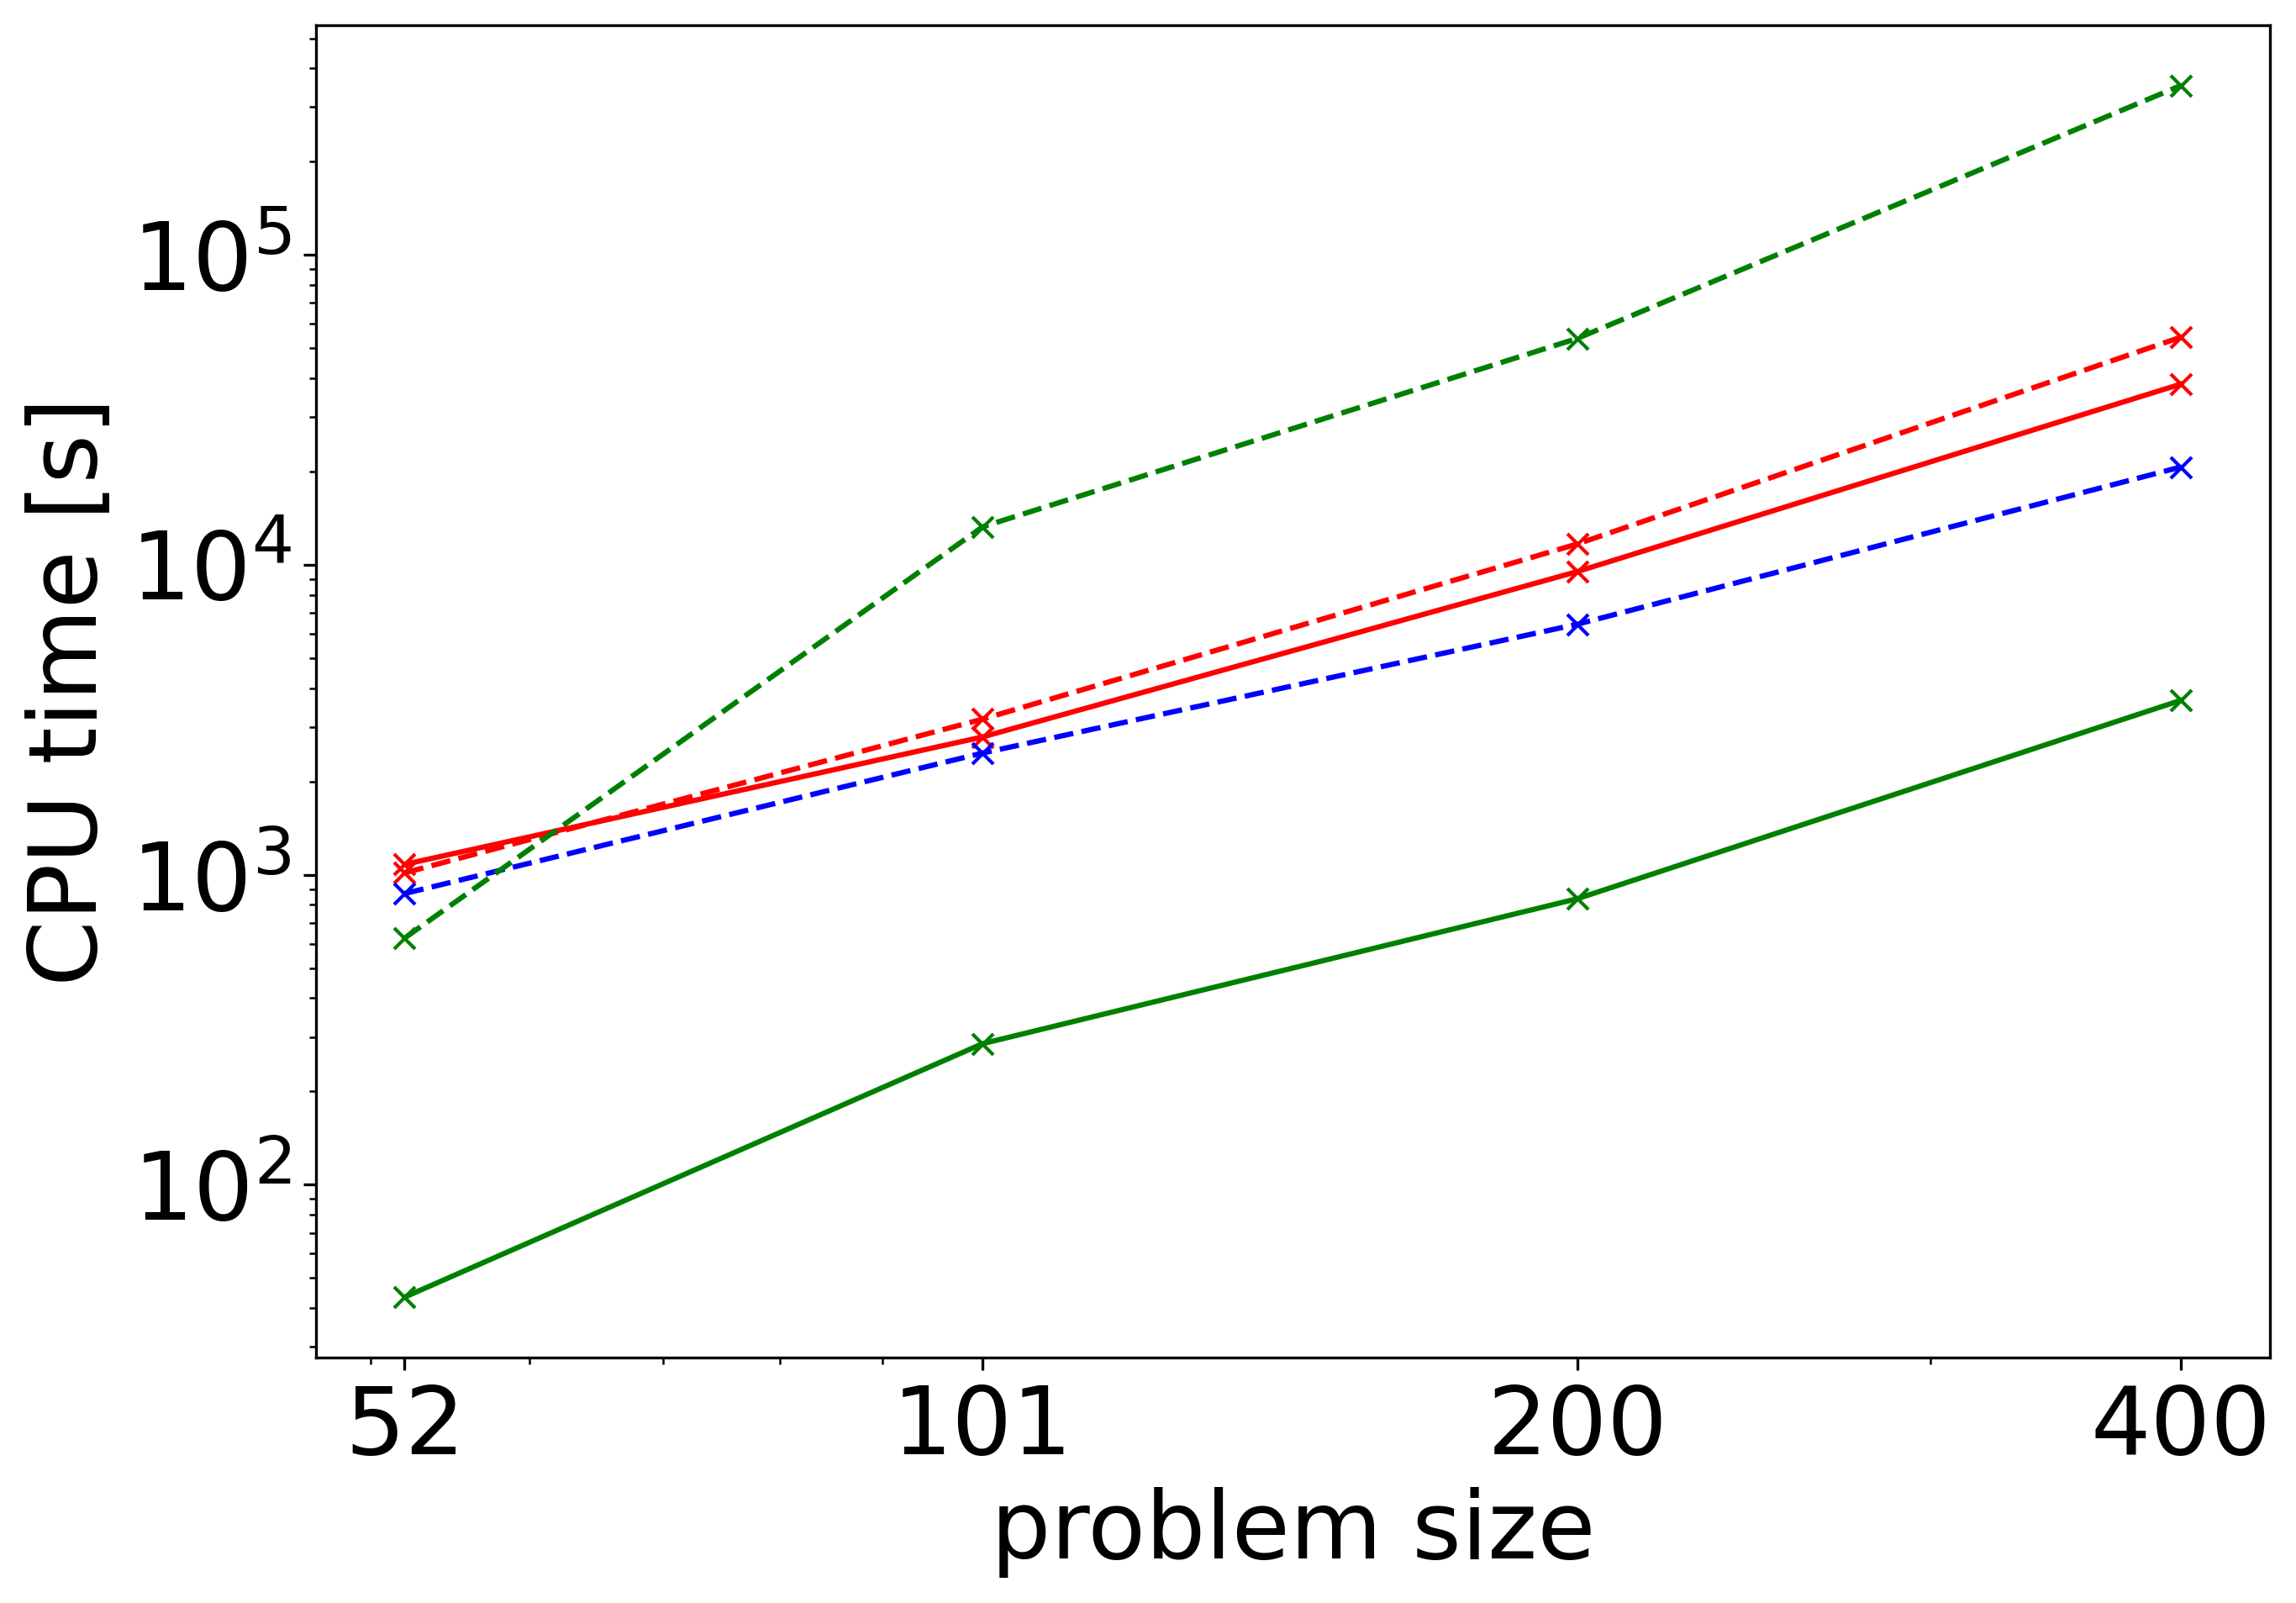
\includegraphics[width=1\textwidth]{images/TANDEM_CPU_Time_solving.png}
		\subcaption{Execution time of the \\ solving phase } 
		\label{fig:scalabilty_executionTimes__solveTime}
	\end{subfigure}
	\caption{Measured CPU times of the RHS evaluation, the initialization and the main solving phases for each combination of formulation and time integration method on different problem sizes.}
	\label{fig:scalabilty_executionTimes}
\end{figure}

Because the explicit 2nd order ODE does not require solving the DG problem in each RHS evaluation, the execution time is about 30 times shorter than using the explicit 1st order ODE formulation. However, this does not hold for the implicit 2nd order ODE, which is as slow as its 1st order counterparts. It seems that setting up the Jacobian matrix and applying the GMRES scheme is much more expensive than for 1st order methods. Indeed, this matrix has no sparse substructure at all, so every operation is more expensive and scales worse with the problem size. Among the 1st order formulations, the explicit ODE approach performs the best. The overhead due to calculating the Jacobian matrix and performing the GMRES iteration explains the difference to the implicit ODE approach, which takes increasingly longer per RHS evaluation. The trick for the DAE formulation from \autoref{ssec:iterative_solver_Jacobian} to apply GMRES only on a dense subsystem yields positive results: its execution time per RHS evaluation remains below the implicit 1st order ODE approach and it scales much better. \\
It can be seen in \autoref{fig:scalabilty_executionTimes__initializationTime} that the initialization phase takes similarly long with all approaches, except for the explicit 1st order ODE, which does not need to initialize any constant Jacobian matrices. Compared to the execution time of the solve phase, it seems to be small in all cases, but for larger domains, the initialization phase might be a major performance bottleneck, especially for short simulations. For the domain with 101 fault elements and the explicit 2nd order approach, 4\% of the total execution time is spent in the initialization, but with 400 fault elements, the ratio is already at about 7\%. On the other hand, for the explicit 1st order ODE, the initialization phase accounts only for 0.04\% of the total execution time independent of the problem size to calculate the initial solution vector. \\
At the start of this thesis, only the explicit 1st order ODE was available in {\ttfamily tandem}. In \autoref{tab:Speedup_Scalability}, the total execution time of all newly implemented approaches is compared to the original reference implementation. A simple implicit treatment of the 1st order ODE decreases eventually the total number of timesteps but produces too much overhead with the Jacobian matrix to accelerate the simulation. The DAE approach is already much more promising as the Jacobian matrix can be reduced to a smaller dense subsystem and the convergence speed of the Newton iteration does not worsen if the problem size increases. However, the best method is by far the explicit 2nd order ODE. The high amount of required timesteps observed in \autoref{ssec:Results_scalability_timestepSizes} is largely compensated by the fast evaluation of the RHS. On the other hand, the implicit 2nd order ODE is not a wise choice, because it combines the disadvantages of a large, badly scaling number of timesteps with an expensive evaluation of the Jacobian matrix and the GMRES scheme. \\

\begin{table}[H]
	\centering 
	\begin{tabular}{ | c | c c c c |}
		\hline	
									 & $n=52$	& $n=101$ 	& $n=200$ 	& $n=400$\\ \hline
		1st order ODE (BDF)			 & 0.94 		& 1.15		& 1.23		& 1.43 	 \\  
		extended DAE  (BDF) 		 & 0.81 		& 0.89 		& 0.67		& 0.55   \\
		2nd order ODE (BDF)          & 0.28 		& 1.21 		& 1.33		& 2.62   \\
		\textit{1st order ODE (RK)}  & \textit{1.00} 		& \textit{1.00}		& \textit{1.00}		& \textit{1.00}   \\  
		2nd order ODE (RK) 			 & 0.04 		& 0.11 		& 0.09		& 0.10   \\ \hline
	\end{tabular}
	\caption{Ratio of the total execution time to the explicit 1st order ODE}
	\label{tab:Speedup_Scalability}
\end{table}

The explicit second order ODE keeps a constant speedup of about 10 compared to the original implementation. This is the best result for the tested scenarios, but it might well be that for higher fault resolutions, the extended DAE formulation performs the best. Indeed, its speedup increases with the problem size, from 1.1 with 101 fault elements to 1.8 with 400 fault elements. In \autoref{fig:scalabilty_executionTimes__solveTime}, it can be seen that the extended DAE formulation has the smallest slope, so if this trend continues, it would be the fastest method.


\section{Towards an ideal model}
\label{sec:Results_towardsAnIdealModel}
An ideal formulation would combine the speed of the 2nd order ODE with the scalability of the extended DAE formulation. For that, a way is needed to compute the shear stress $\tau$ without solving the DG problem. It can be achieved with the same trick used to set up the 2nd order ODE formulation: $\tau$ depends linearly on the time and on the slip. Thus, we can just set: 
\begin{equation}
	\tau = \tau_0 + \pdv{\tau}{t}t + \pdv{\tau}{S}S
\end{equation}
The two partial derivatives are constant terms that can be initialized at the beginning of the simulation and the friction law can be calculated without solving the DG problem anymore at each RHS evaluation. This strategy was not implemented nor tested but appears to be promising for further development.
